\subsubsection{Kinematic Observables} \label{sec:KinematicObservables}

The differential cross section measurements are performed as a function of the kinematic properties of the four-lepton system and the jet multiplicity, and
are unfolded to the particle level.
In this document, regarding the kinematic properties of the four-lepton system, the results are reported for the transverse momentum and
rapidity of the four-lepton system ($\pt({\rm H})$ or $\pt(4\ell)$, $|y({\rm H})|$ or $|y(4\ell)|$), N(jets), and $\pt({\rm jet})$ which probe the production mechanism.
%,
%as well as for the invariant mass of the two leading leptons $m(\mathrm{Z}_{1})$, the invariant mass of the two sub-leading leptons $m(\mathrm{Z}_{2})$ and
%the five helicity angles in the Collins-Soper 
%frame~\cite{Collins:1977iv} ($|\cos(\theta)|$, $|\cos(\theta_{1})|$, $|\cos(\theta_{2})|$, $|\Phi|$, $|\Phi_{1}|$), which are also related to properties
%of the decay mechanism. 
The binning boundaries for each kinematic observable have been optimized in order to have a similar expected measured cross-section for every bin.
%The same set of observables are used in the differential cross section measurements for both $\Hllll$ and $\Zllll$ decays.

\subsubsection{Background Model} \label{sec:BackgroundDifferential}
In order to perform the differential measurements, the background is to be subtracted at the reconstruction level for each bin
of the considered observable.
In general, the background mass spectrum shape is not the same in all bins of the considered observable because the background does not have a resonance
structure. The mass spectrum also can have non-negligible correlation with the observables. 
%For example, in we consider the observable m${}_{Z2}$, the 
%background events tend to have a larger four-lepton mass  for larger m${}_{Z2}$ values.
\par 
In case of the irreducible backgrounds, the four-lepton mass spectra are modeled as the $m_{4\ell}$ template shapes using simulated events
for each bin of the observable considered for the measurement. Similarly, in case of the reducible backgrounds the templates are built from the control 
regions in the data. This procedure is similar to the one described and used in the Ref.~\cite{Chatrchyan:2013mxa}.
\par 
%Figure\ref{fig:bkg-pT4l-qqZZ-ZX-main} shows the $qqZZ$ and $Z+X$ background mass spectra in different bins defined by the $p_{T}(4\ell)$ observable at 
%reconstruction level. From the plots, one can see that there is clear discrepancy in the shape of the mass spectrum among different 
%bins. Table \ref{tab:fractions_pT4l-main} shows estimated fraction of background events in each bin of $\pt(4\ell)$, for each final state. Mass spectra
%of $qqZZ$, $\Pg\Pg\Z\Z$ and $Z+X$ backgrounds in bins of all observables considered for the differential measurements are shown in the
%Appendix~\ref{app:bkginputs_shapes}: for $\pt(4\ell)$ in Figures~\ref{fig:bkg-pT4l-qqZZ-ZX} and~\ref{fig:bkg-pT4l-qqZZ-ggZZ};  for $|y(4\ell)|$ in
%Figures~\ref{fig:bkg-rapidity4l-qqZZ-ZX} and~\ref{fig:bkg-rapidity4l-qqZZ-ggZZ},
%%for $|\cos \theta^{*}|$ in Figures~\ref{fig:bkg-cosThetaStar-qqZZ-ZX}
%%and~\ref{fig:bkg-cosThetaStar-qqZZ-ggZZ}, for $m(\mathrm{Z}_{2})$ in Figures~\ref{fig:bkg-massZ2-qqZZ-ZX} and~\ref{fig:bkg-massZ2-qqZZ-ggZZ}, 
%for $N_{\rm jets}$ in Figures~\ref{fig:bkg-njets_reco_pt30_eta4p7-qqZZ-ZX} and~\ref{fig:bkg-njets_reco_pt30_eta4p7-qqZZ-ggZZ}). 
%Similarly, fractions of background events in each bin of $\pt(4\ell)$, $m(\mathrm{Z}_{2})$, $N_{\rm jets}$, $|y(4\ell)|$  and  $|\cos \theta^{*}|$~are presented in 
Fractions of background events in each bin of $\pt(4\ell)$ ~are presented in Table \ref{tab:fractions_pT4l}. 
%of background events in each bin of $\pt(4\ell)$ are presented in Tables~\ref{tab:fractions_pT4l}. 
%of background events in each bin of $\pt(4\ell)$, $N_{\rm jets}$, $|y(4\ell)|$  and $\pt({\rm jet})$ are presented in Tables~\ref{tab:fractions_pT4l},~\ref{tab:fractions_massZ2},~\ref{tab:fractions_rapidity4l},~\ref{tab:fractions_cosThetaStar} 
%and~\ref{tab:fractions_njets_reco_pt30_eta4p7}  respectively in the Appendix~\ref{app:bkginputs_fractions}.


\begin{table}[!h!tb]
\begin{center}
%\small
\scriptsize
%\tiny
    \caption{
        Estimated fraction of background events in each bin of $\pt(4\ell)$, for each final state using 2018 samples.
%\label{tab:fractions_pT4l-main}
\label{tab:fractions_pT4l}
}
%\begin{tabular}{|l|c|c|c|c|c|}
\begin{tabular}{|l|c|c|c|c|c|c|c|c|}
\hline
%Background & final state & $0\leq$$\pt(4\ell)$$<15$ & $15\leq$$\pt(4\ell)$$<30$ & $30\leq$$\pt(4\ell)$$<45$ & $45\leq$$\pt(4\ell)$$<80$ & $80\leq$$\pt(4\ell)$$<120$ & $120\leq$$\pt(4\ell)$$<200$ & $200\leq$$\pt(4\ell)$$<13000$ \\ \hline
Background & final state & $0-15$ & $15-30$ & $30-45$ & $45-80$ & $80-120$ & $120-200$ & $200-13000$ \\ \hline
qqZZ& $2e2\mu$  & 0.483668  & 0.239196  & 0.130151  & 0.105276 & 0.0266332  & 0.011809  & 0.00326633 \\
qqZZ& $4e$  & 0.459665  & 0.234399  & 0.136986  & 0.114916 & 0.0388128  & 0.00989346  & 0.00532725 \\
qqZZ& $4\mu$  & 0.492632  & 0.241203  & 0.110977  & 0.109173 & 0.0297744  & 0.0129323  & 0.00330827 \\
\hline
ggZZ& $2e2\mu$  &  0.310446 & 0.309859  & 0.191901  & 0.168134 & 0.0187793  & 0.000880282  & 0.0 \\
ggZZ& $4e$  & 0.3085  & 0.306332  & 0.19247  & 0.17433 & 0.0169994  & 0.00136908  & 0.0 \\
ggZZ& $4\mu$  & 0.321332  & 0.319311  & 0.194863  & 0.150987 & 0.0128703  & 0.000638196  & 0.0 \\
\hline
Z+X (CR)& 4l  & 0.0992521  & 0.211153  & 0.209307 & 0.305327  & 0.120303  & 0.0483797 & 0.00627828 \\
\hline
\end{tabular}
\normalsize
\end{center}
\end{table}
%%%%%%%%%%%%%
%\begin{figure}[!ht]
%  \begin{center}
%
%    \subfigure[$0.0 < \pt(4\ell) < 15.0$]{
%      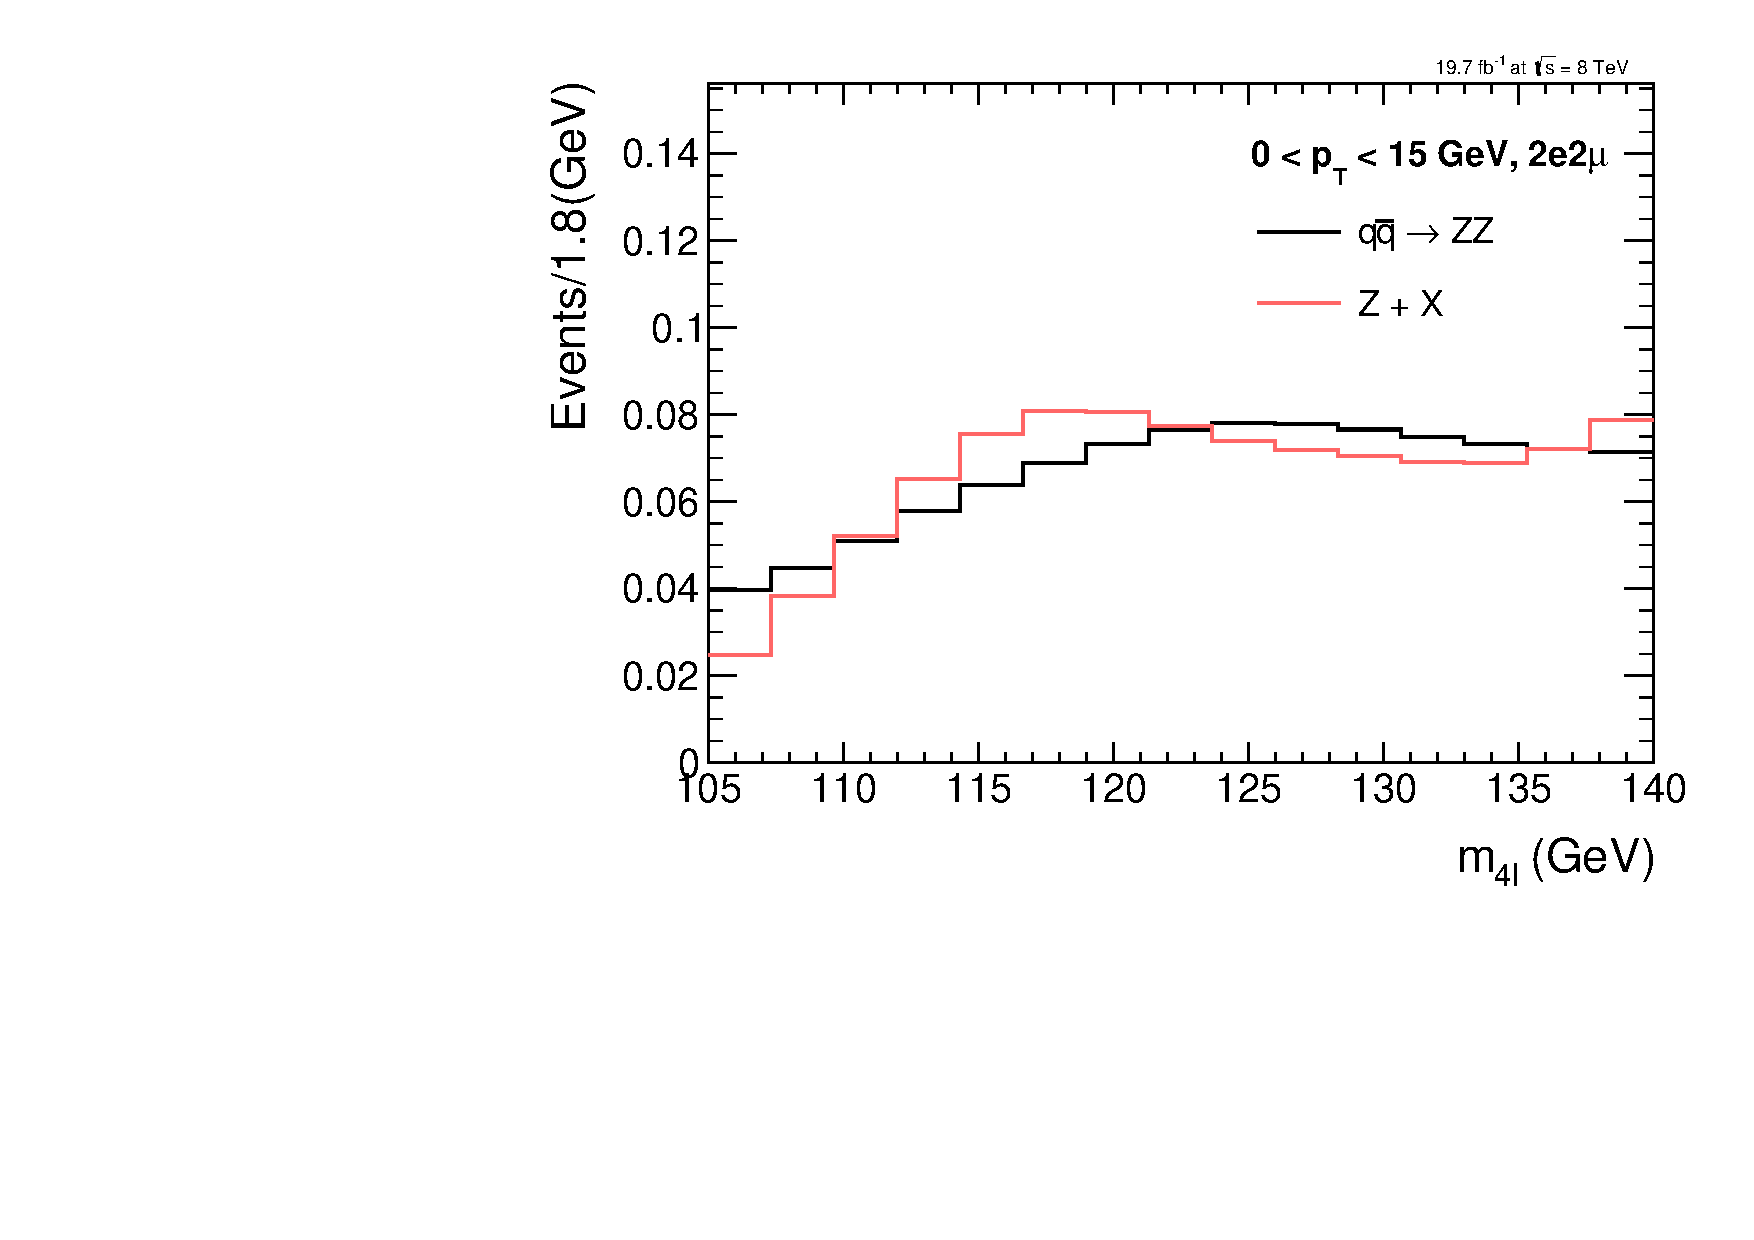
\includegraphics[width=0.3\textwidth,angle=0]{Appendix/figures/XSTemplates_2e2mu_pT4l_0_15_qqZZ_ZJetsCR.pdf}
%    }
%    \subfigure[$0.0< \pt(4\ell) < 15.0$]{
%      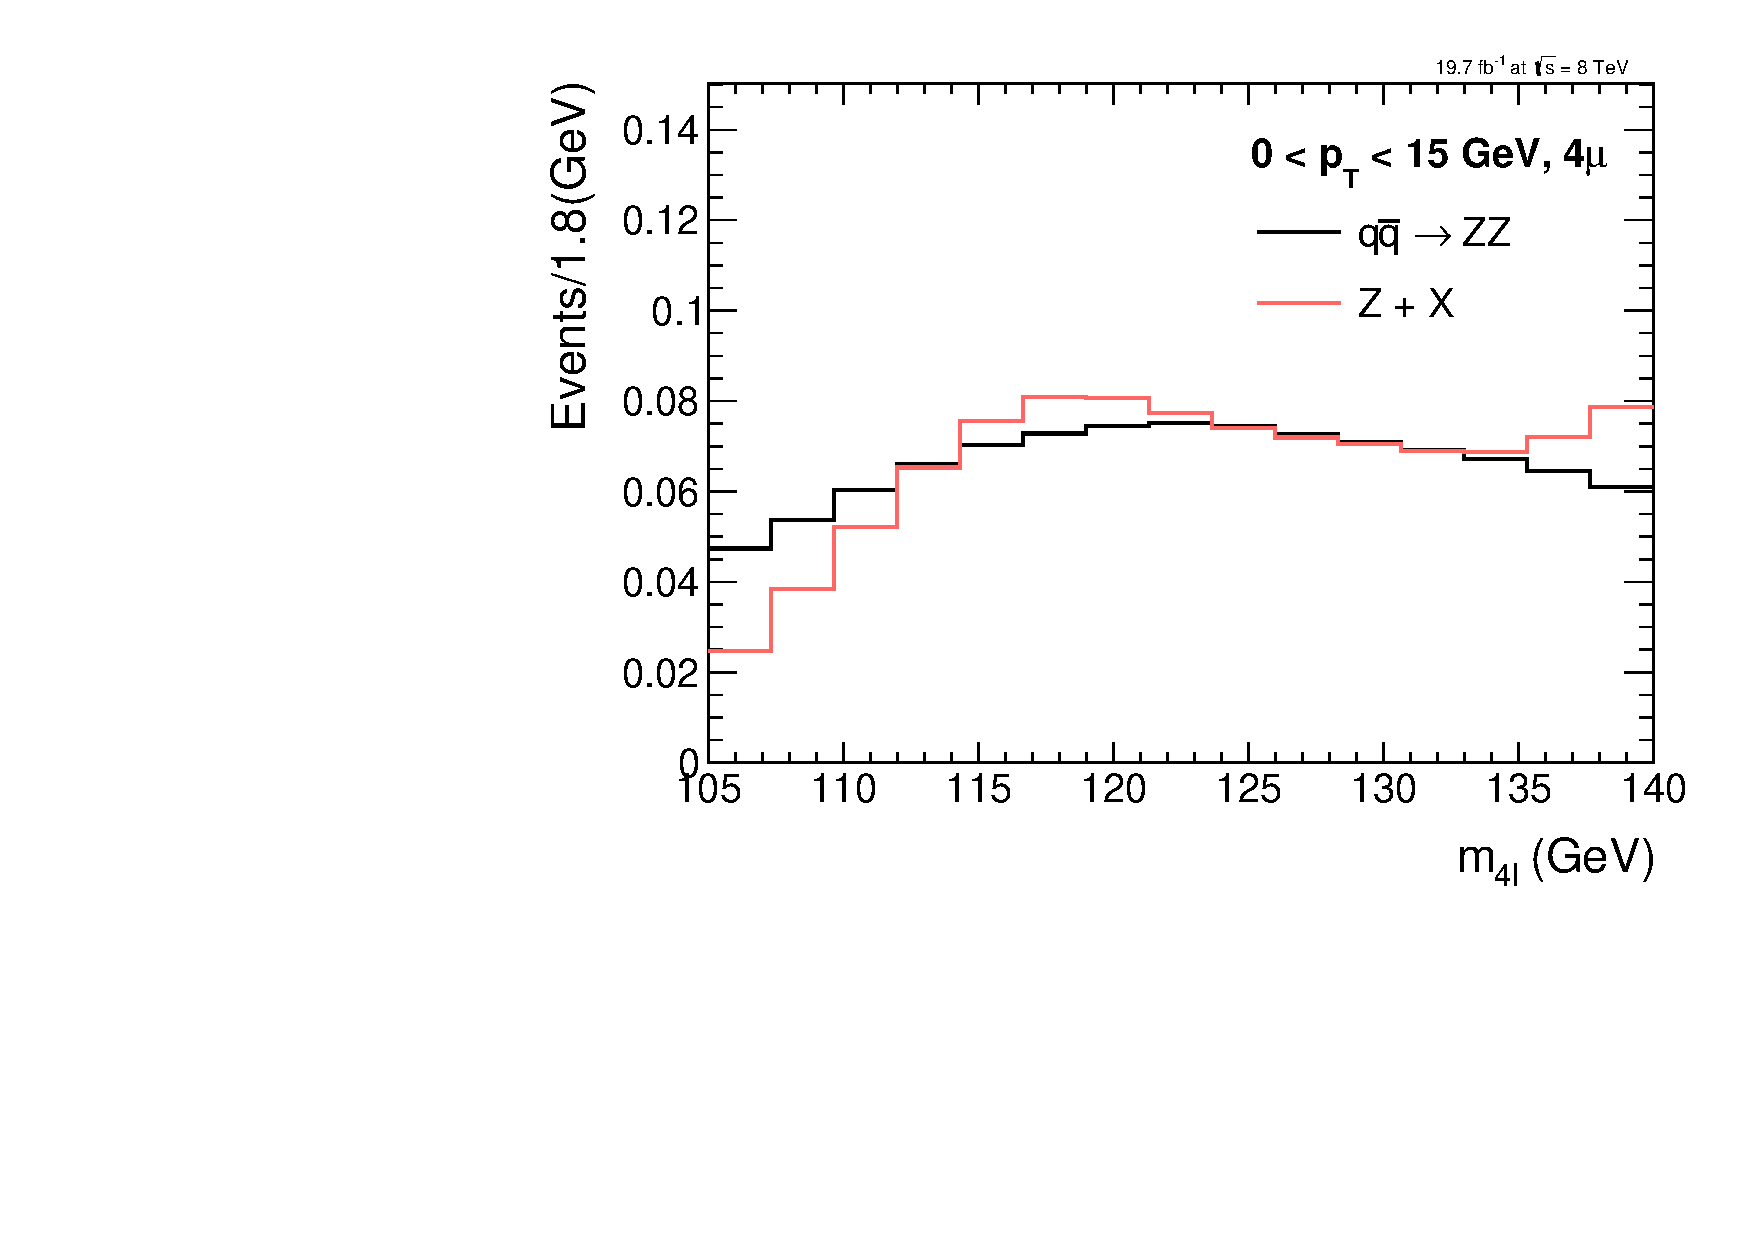
\includegraphics[width=0.3\textwidth,angle=0]{Appendix/figures/XSTemplates_4mu_pT4l_0_15_qqZZ_ZJetsCR.pdf}
%    }
%    \subfigure[$0.0 < \pt(4\ell) < 15.0$]{
%      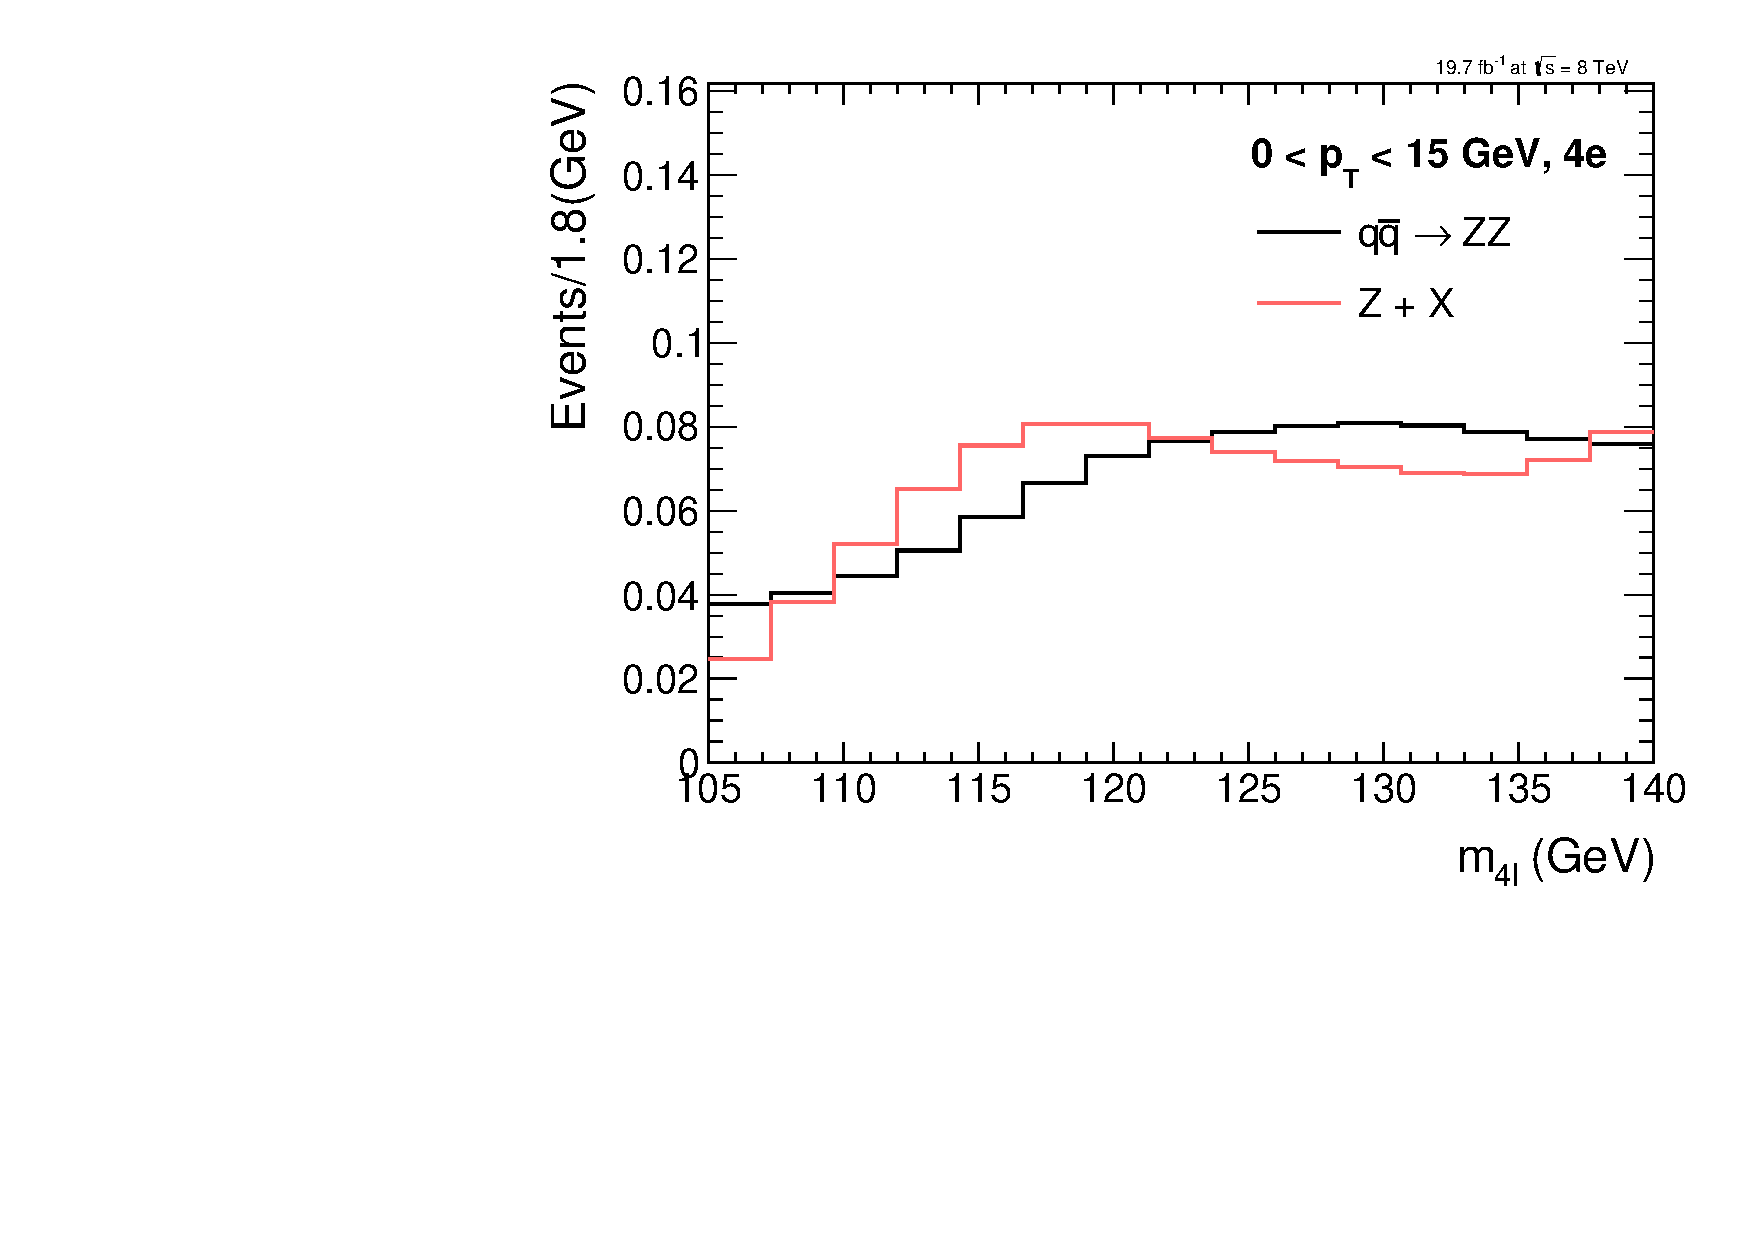
\includegraphics[width=0.3\textwidth,angle=0]{Appendix/figures/XSTemplates_4e_pT4l_0_15_qqZZ_ZJetsCR.pdf}
%    }    \\
% 
%    \subfigure[$15.0 < \pt(4\ell) < 30.0$]{
%      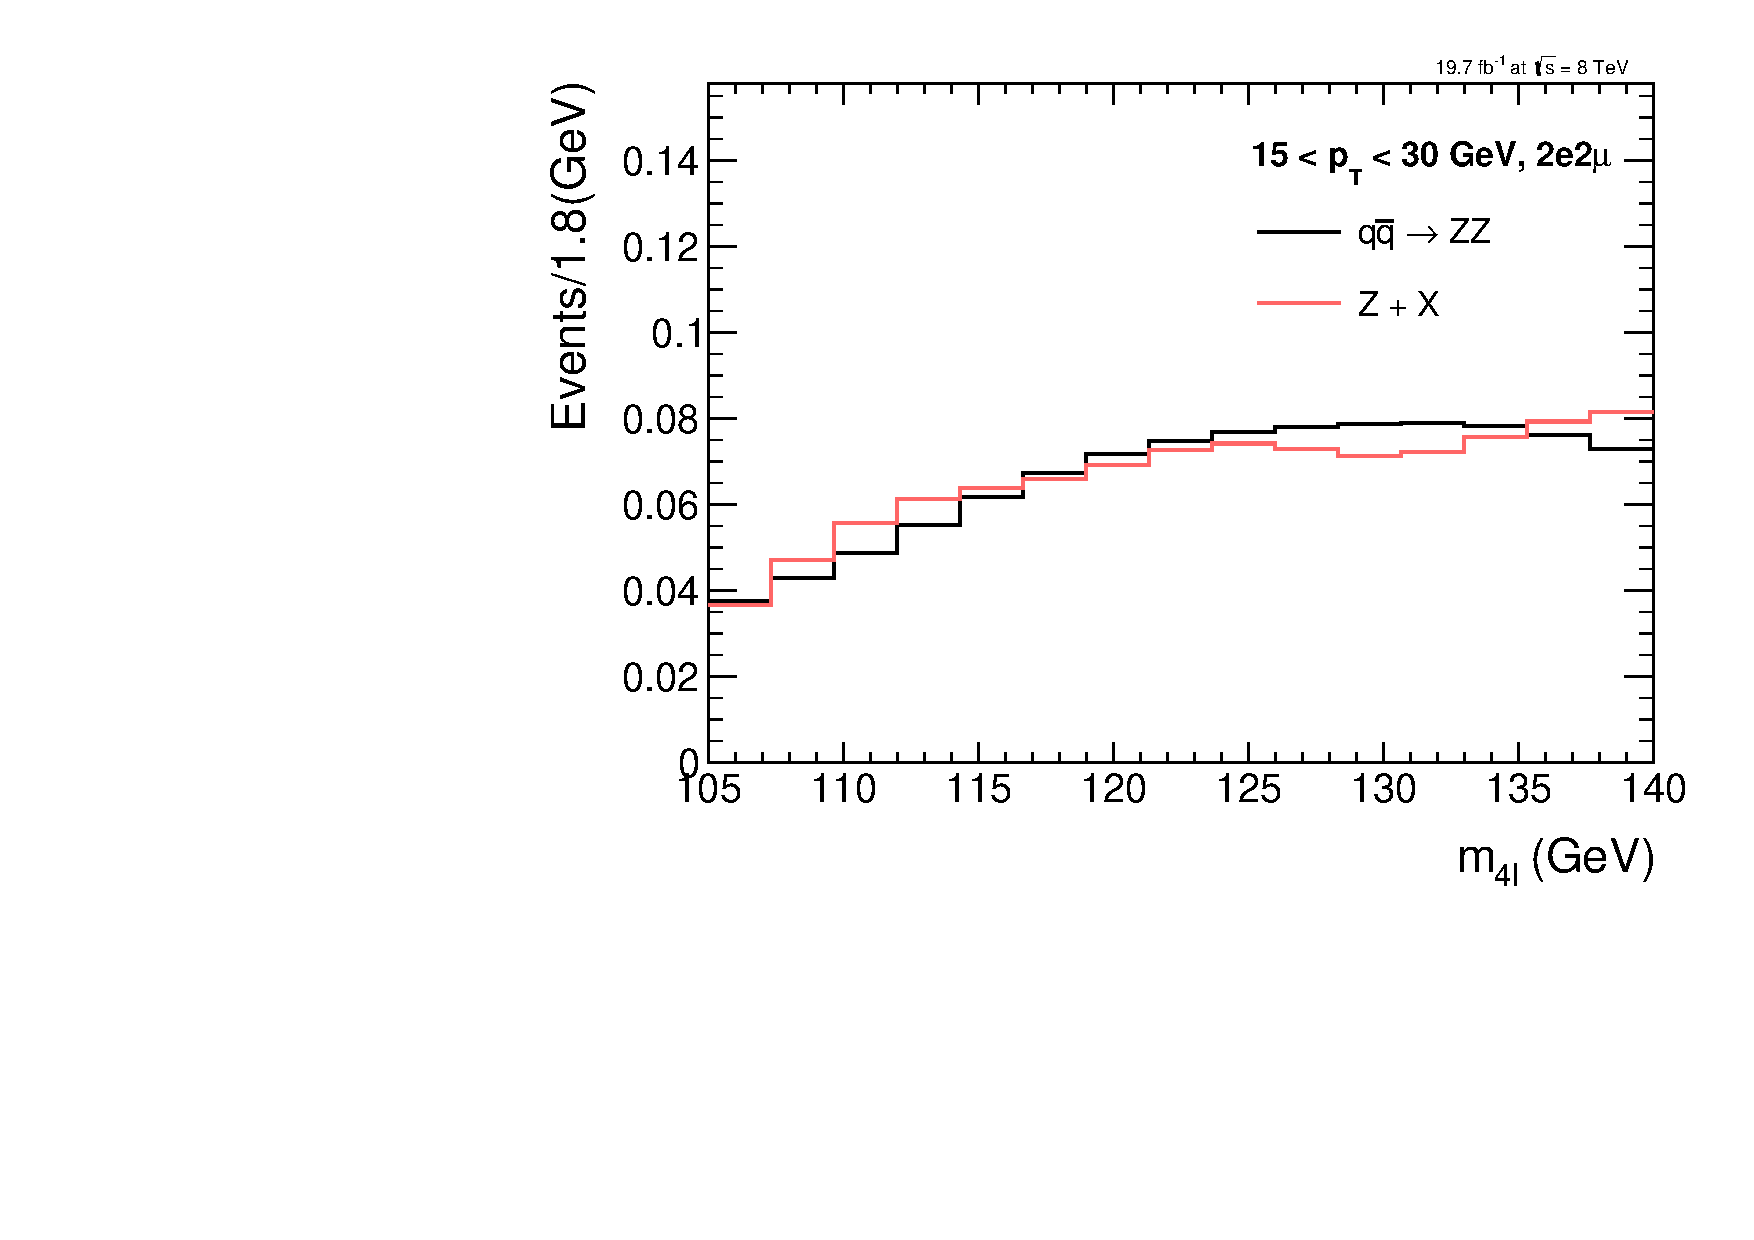
\includegraphics[width=0.3\textwidth,angle=0]{Appendix/figures/XSTemplates_2e2mu_pT4l_15_30_qqZZ_ZJetsCR.pdf}
%    }
%    \subfigure[$15.0 < \pt(4\ell) < 30.0$]{
%      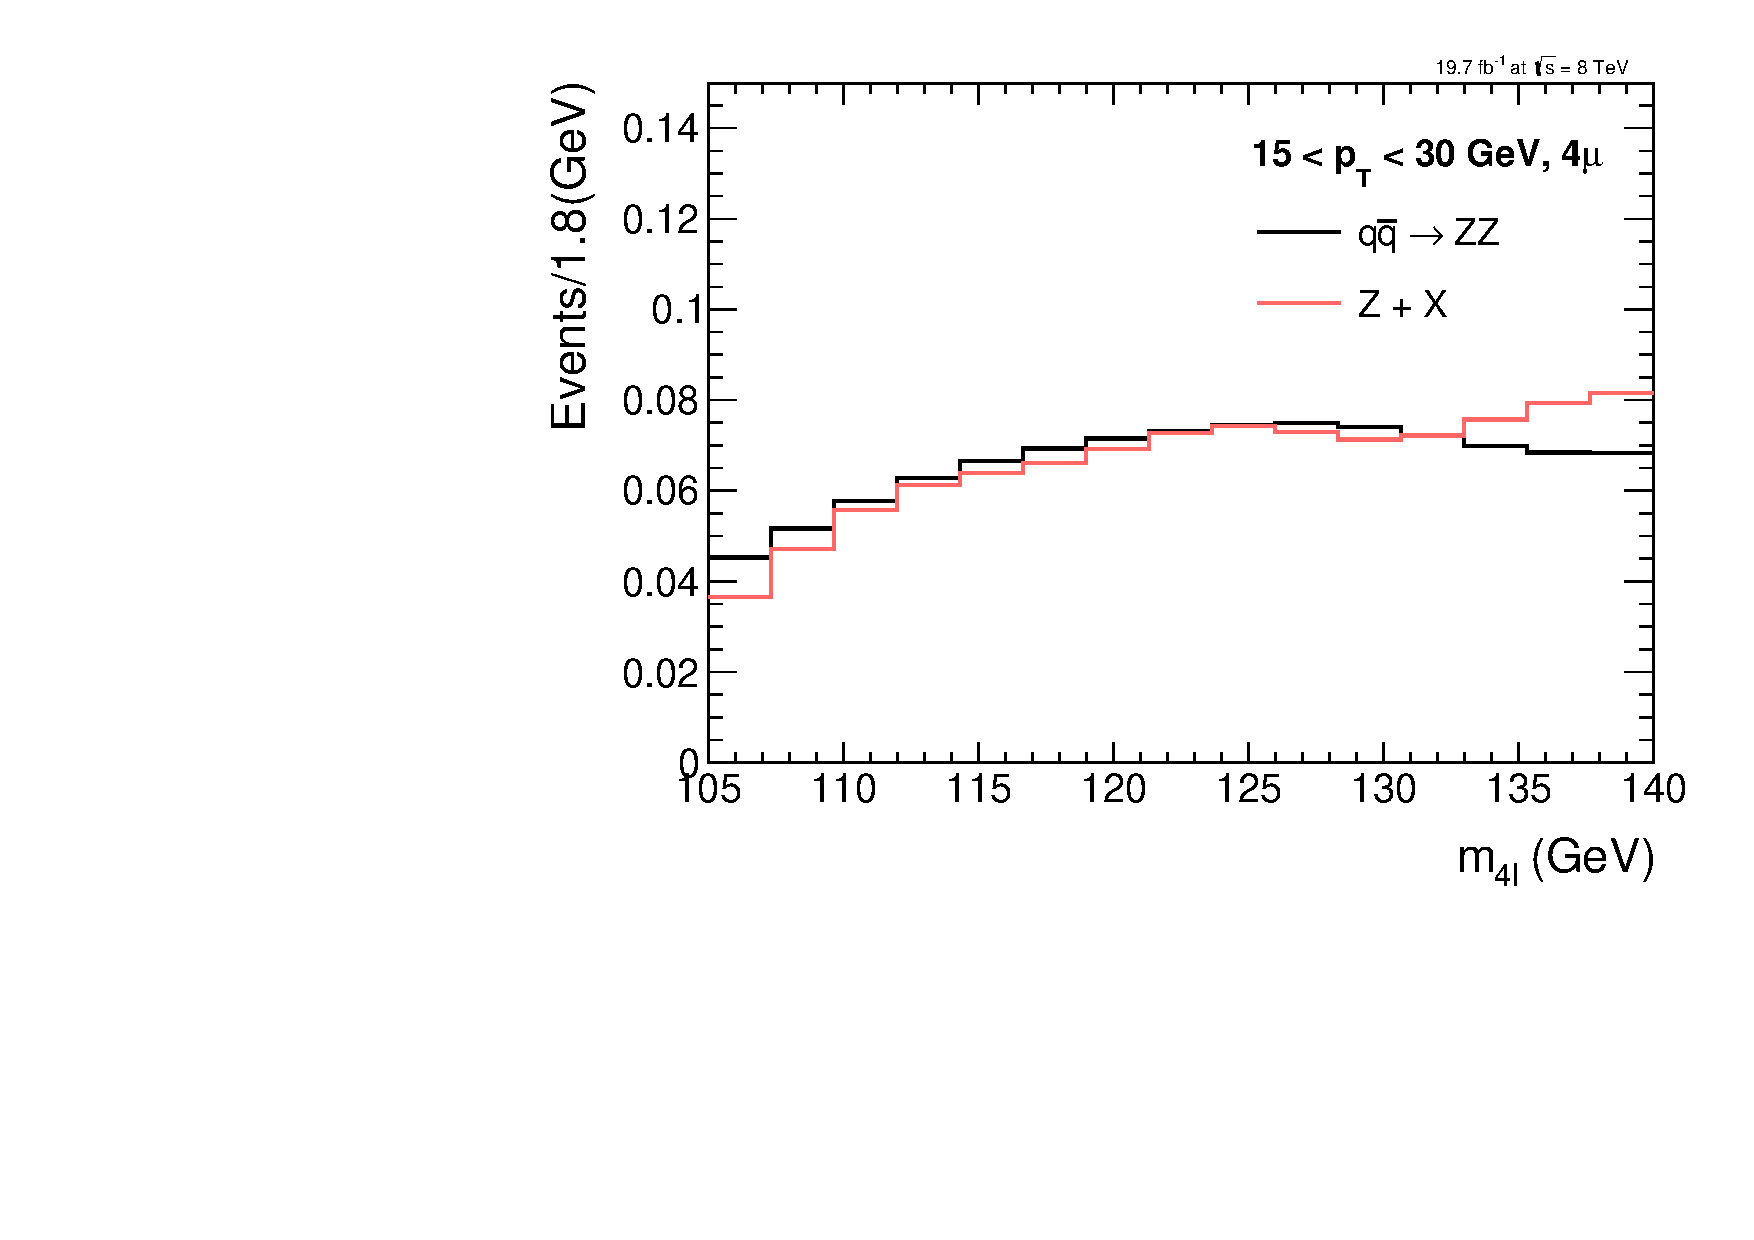
\includegraphics[width=0.3\textwidth,angle=0]{Appendix/figures/XSTemplates_4mu_pT4l_15_30_qqZZ_ZJetsCR.pdf}
%    }
%    \subfigure[$15.0  < \pt(4\ell) < 30.0$]{
%      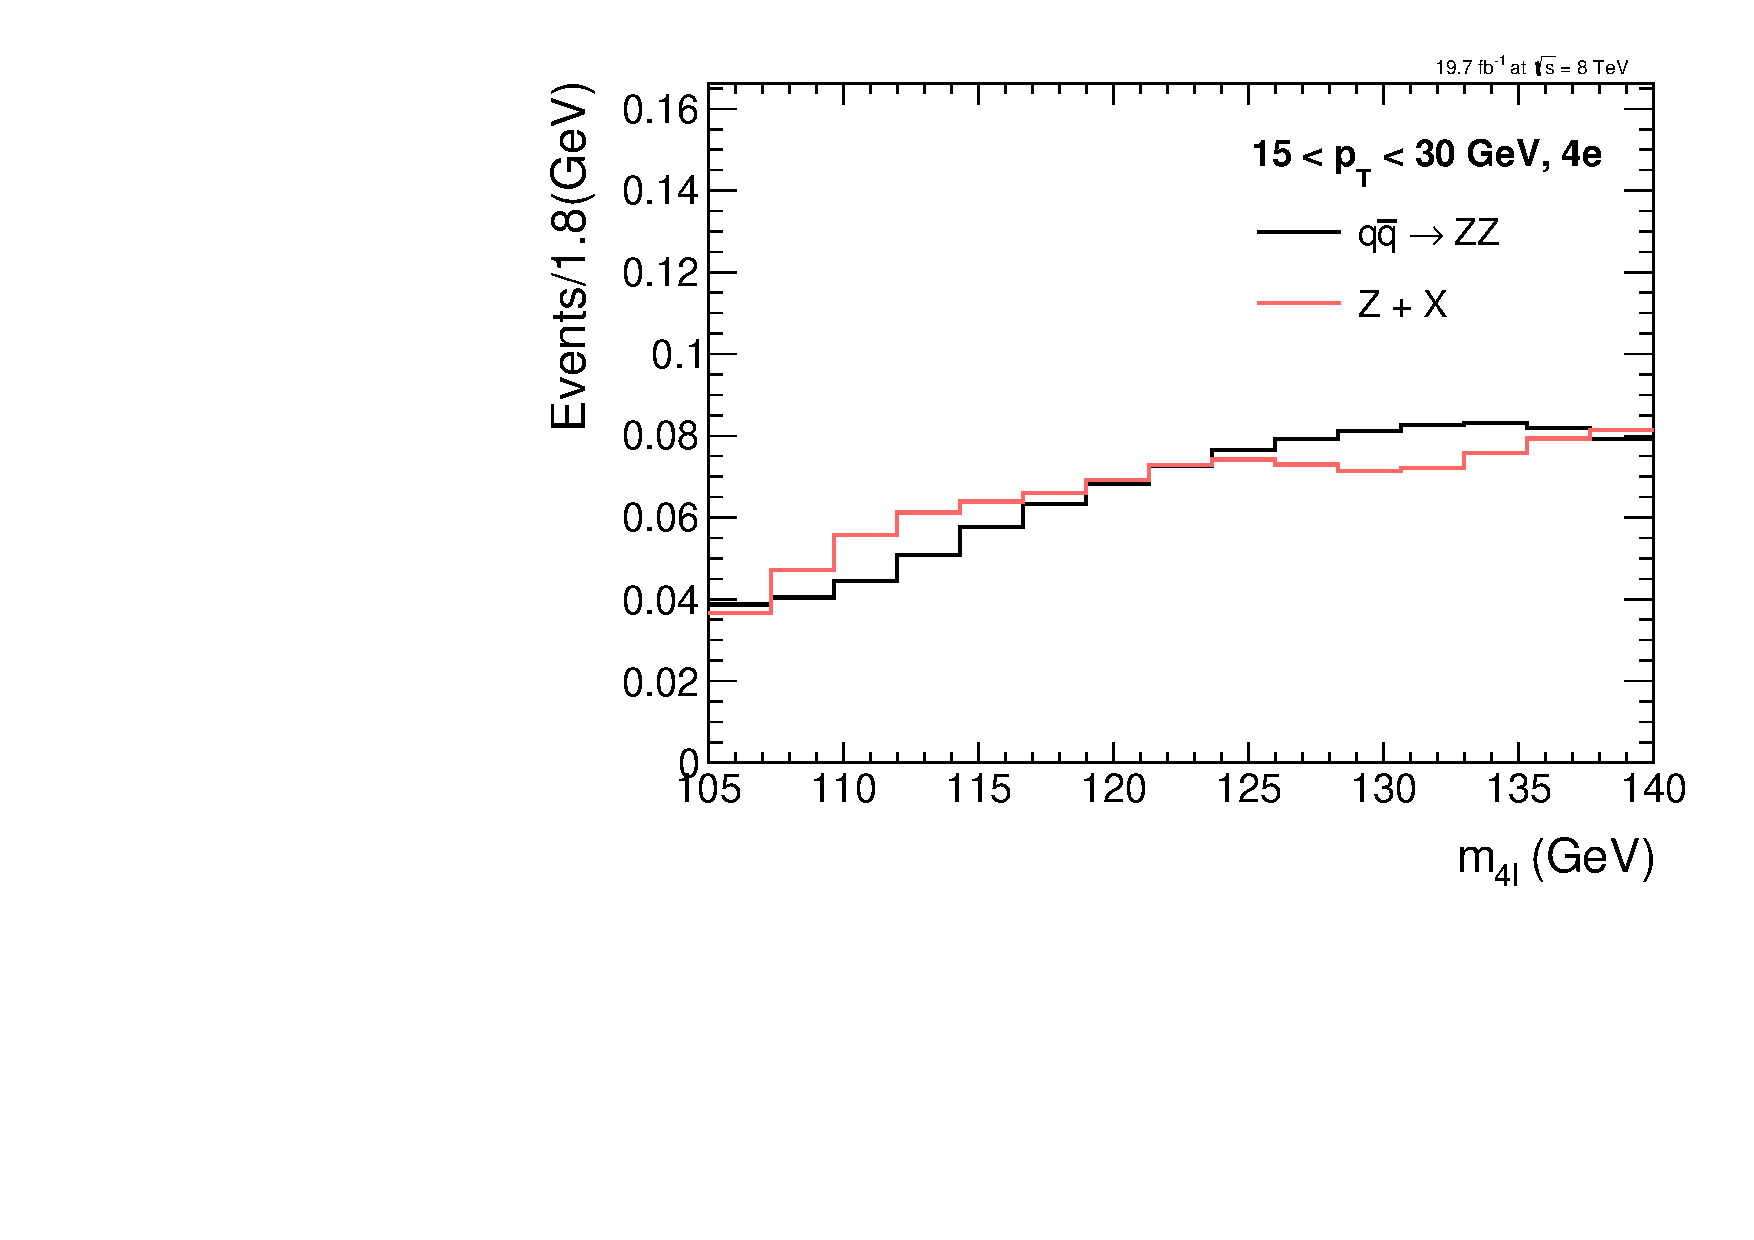
\includegraphics[width=0.3\textwidth,angle=0]{Appendix/figures/XSTemplates_4e_pT4l_15_30_qqZZ_ZJetsCR.pdf}
%    } \\
% 
%    \subfigure[$30.0 < \pt(4\ell) < 60.0$ ]{
%      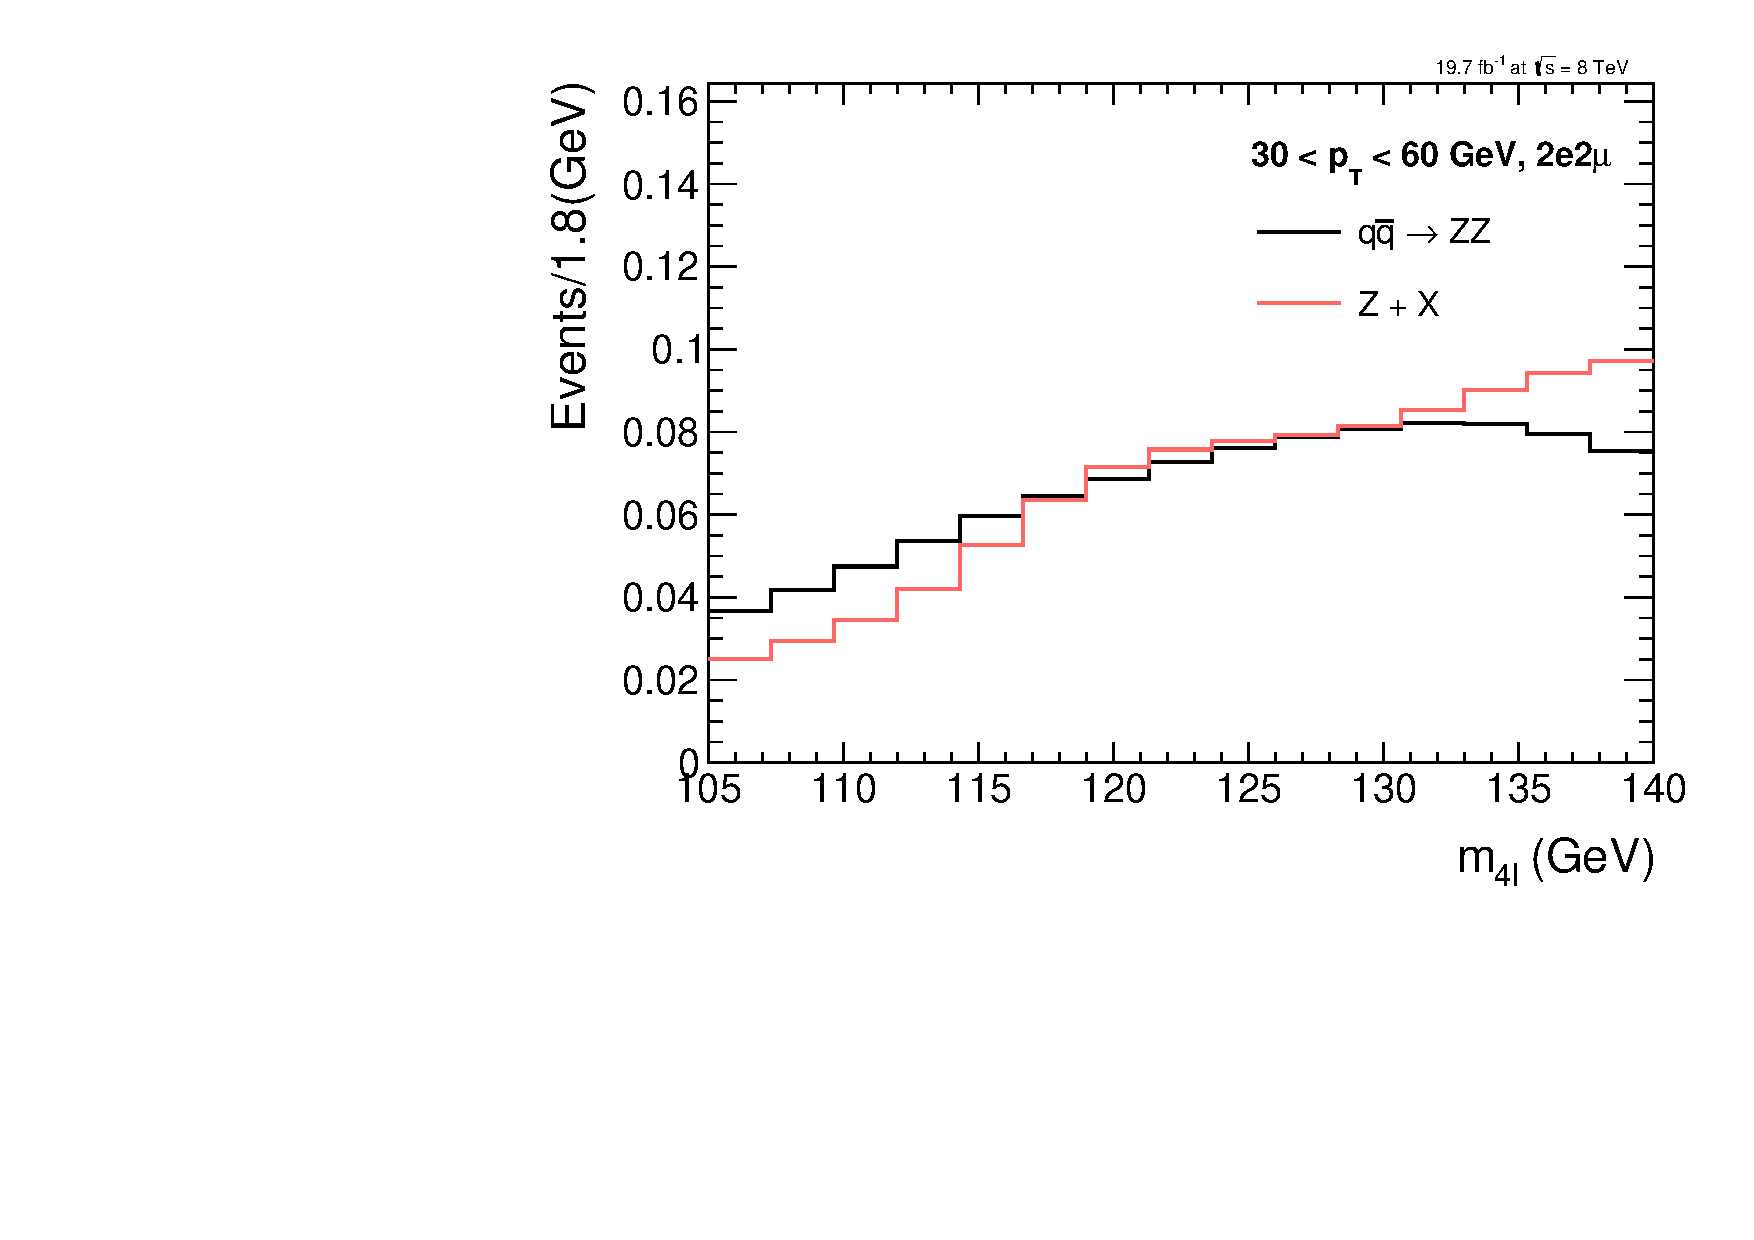
\includegraphics[width=0.3\textwidth,angle=0]{Appendix/figures/XSTemplates_2e2mu_pT4l_30_60_qqZZ_ZJetsCR.pdf}
%    }
%    \subfigure[$30.0 < \pt(4\ell) < 60.0$]{
%      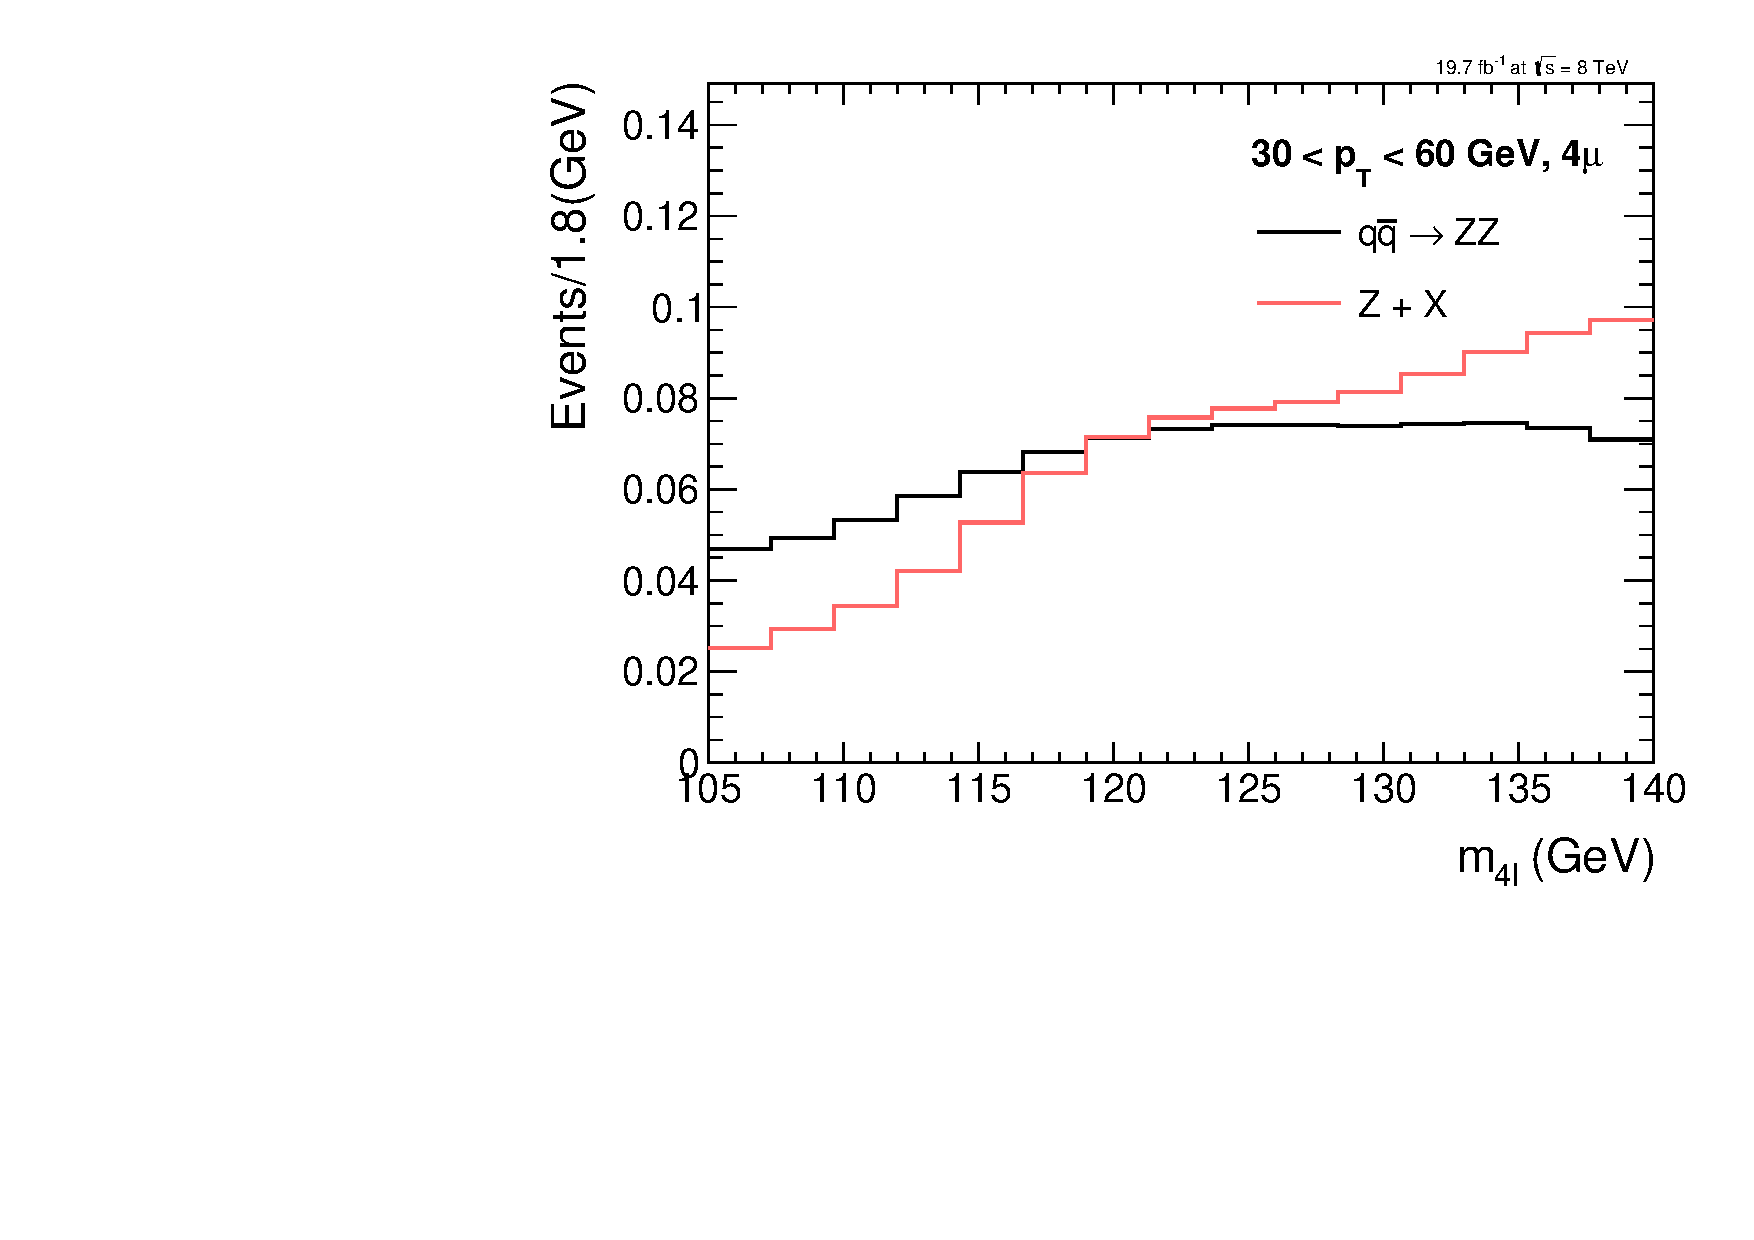
\includegraphics[width=0.3\textwidth,angle=0]{Appendix/figures/XSTemplates_4mu_pT4l_30_60_qqZZ_ZJetsCR.pdf}
%    }
%    \subfigure[$30.0 < \pt(4\ell) < 60.0$]{
%      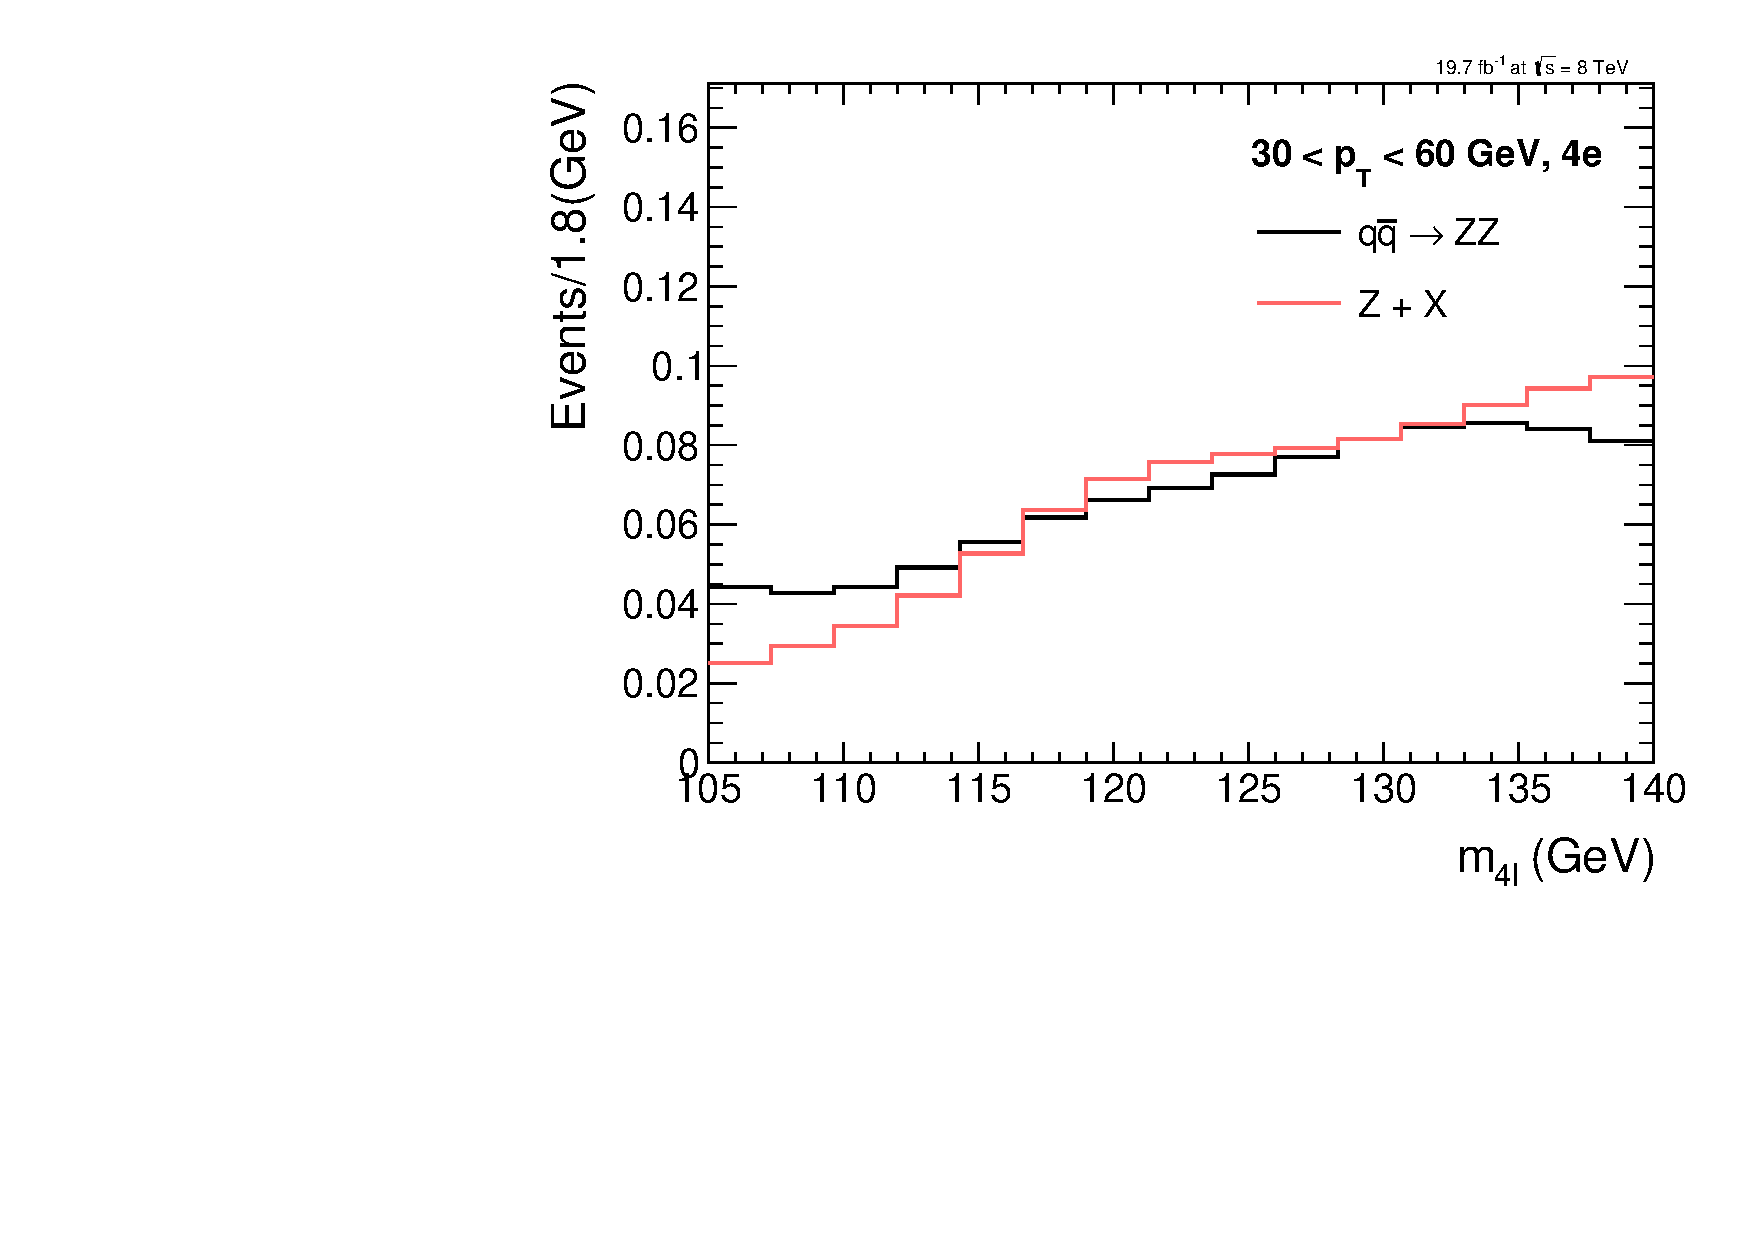
\includegraphics[width=0.3\textwidth,angle=0]{Appendix/figures/XSTemplates_4e_pT4l_30_60_qqZZ_ZJetsCR.pdf}
%    } \\
%
%    \subfigure[$60.0 < \pt(4\ell) < 200.0$]{
%      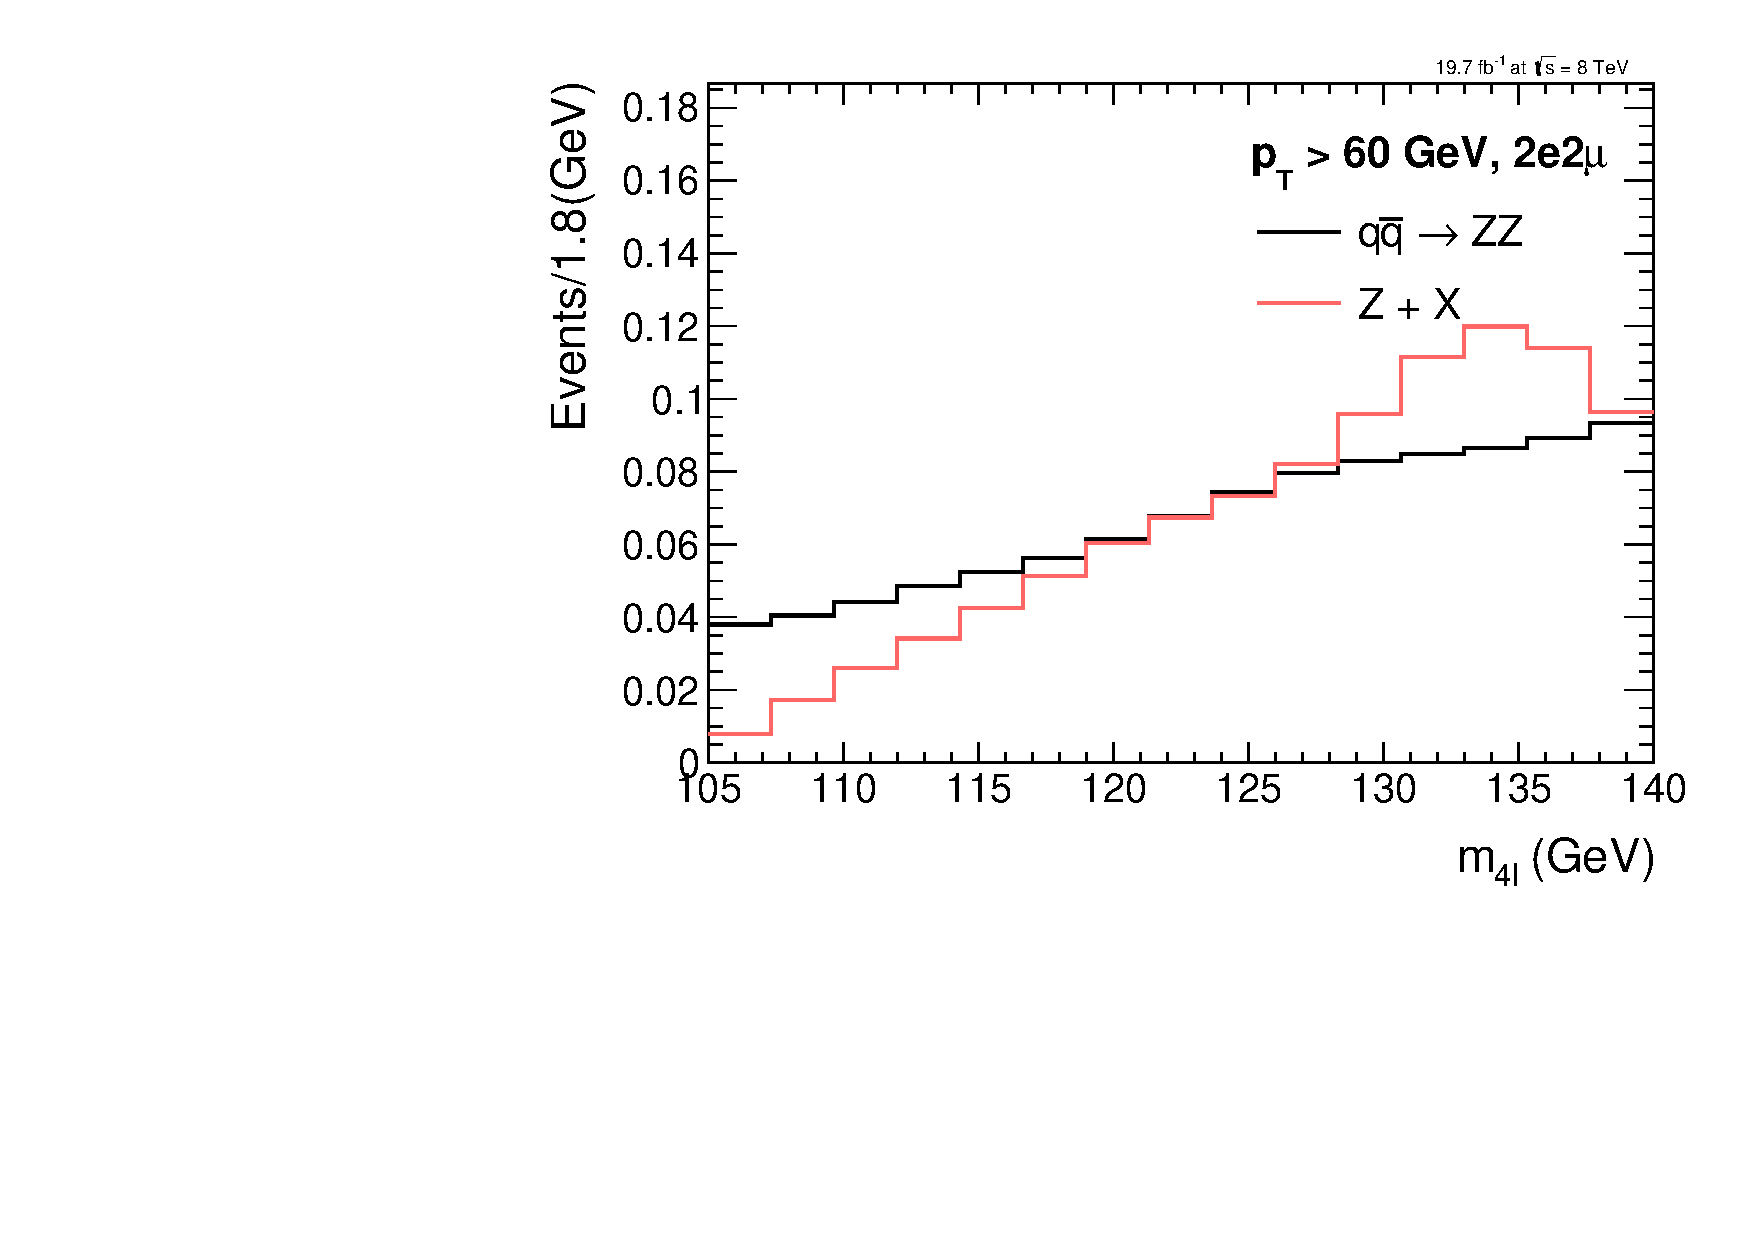
\includegraphics[width=0.3\textwidth,angle=0]{Appendix/figures/XSTemplates_2e2mu_pT4l_60_200_qqZZ_ZJetsCR.pdf}
%    }
%    \subfigure[$60.0 < \pt(4\ell) < 200.0$]{
%      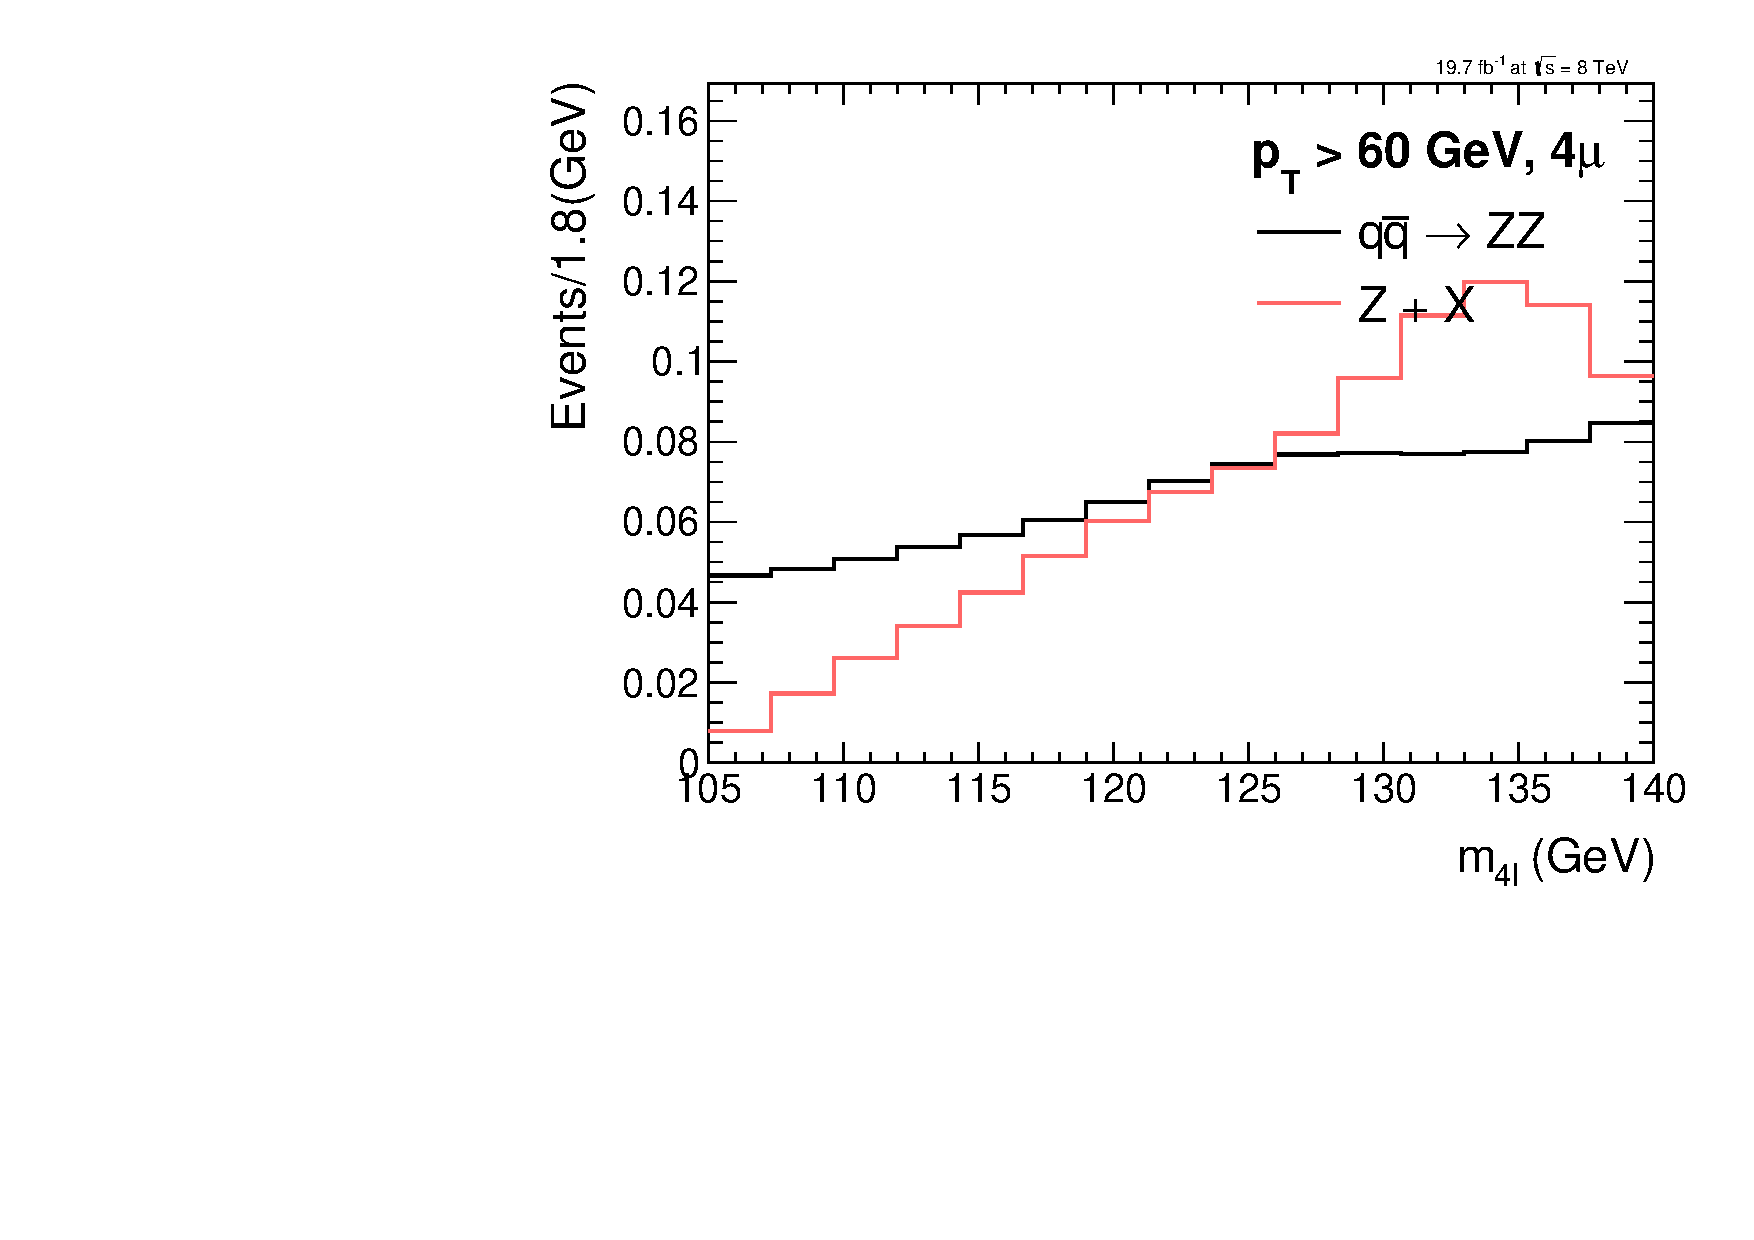
\includegraphics[width=0.3\textwidth,angle=0]{Appendix/figures/XSTemplates_4mu_pT4l_60_200_qqZZ_ZJetsCR.pdf}
%    }
%    \subfigure[$60.0 < \pt(4\ell) < 200.0$]{
%      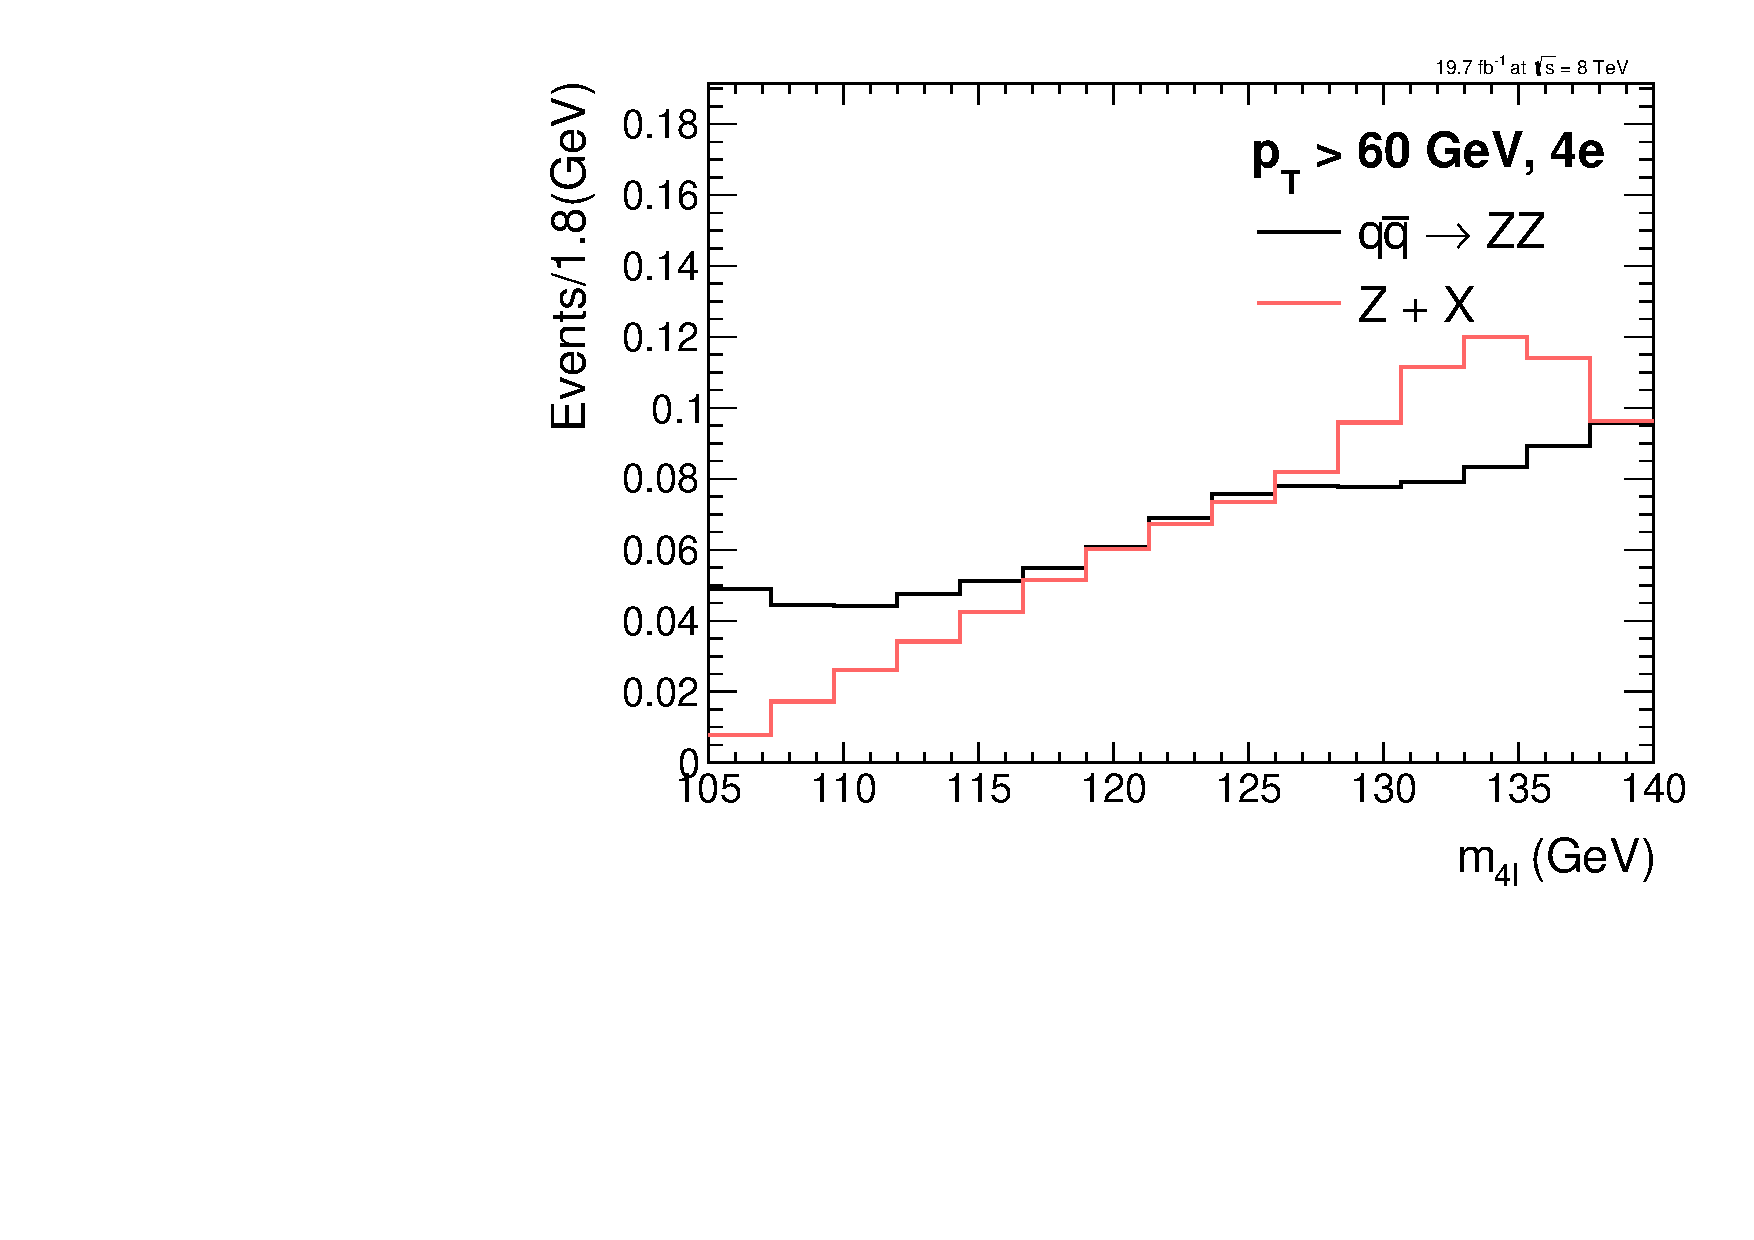
\includegraphics[width=0.3\textwidth,angle=0]{Appendix/figures/XSTemplates_4e_pT4l_60_200_qqZZ_ZJetsCR.pdf}
%    } \\
%
%    \caption{ Distributions of m($4\ell$) for the $qq \rightarrow \mathrm{ZZ}$ and Z+X backgrounds in different bins of $\pt(4\ell)$
%    for three final states: $2e2\mu$(left), $4\mu$(middle) and $4e$(right).}
%  \label{fig:bkg-pT4l-qqZZ-ZX-main}
%
% \end{center}
%\end{figure}

\clearpage

\subsubsection{Signal Model and Statistical Procedure} \label{sec:SignalDifferential}
In order to measure the differential cross sections within the fiducial phase space, we extract the cross sections in the bins of kinematic observables at the fiducial
level following the procedure outlined in Section~\ref{sec:SignalStatProcedure}. To extract the signal yields, the signal mass spectrum is built in each cell
of the response matrix using a double-sided Crytal Ball (CB) function, as was done in Ref.~\cite{Chatrchyan:2013mxa}.
In practice, the same parameters of the CB function are used in each cell and the systematic uncertainties assigned on the energy scale and resolution are 
general enough to cover
the discrepancy of the signal mass spectrum among each cell.
\par
Examples of the fitted signal line shapes for differential bins of $\pt({\rm H})$ from gg$\rightarrow$H ({\sc powheg+JHUgen} 125 $\GeV$ 2018 sample) in the individual
final states are shown in Figure~\ref{fig:sigfits-pT4l-ggH-powheg15-JHUgen-125-maintext}, and examples of the efficiency matrices for $\pt({\rm H})$ for the
$2e2\mu$ final state are shown in Fig~\ref{fig:eff-pT4l-2e2mu-maintext}. Many more examples can be seen in Appendix~\ref{signalinputs}.

%%%%%%%%%5
\begin{figure}[htb]
  \begin{center}
    \subfigure[$0.0 < \pt(\mathrm{H}) < 15.0 $]{
      %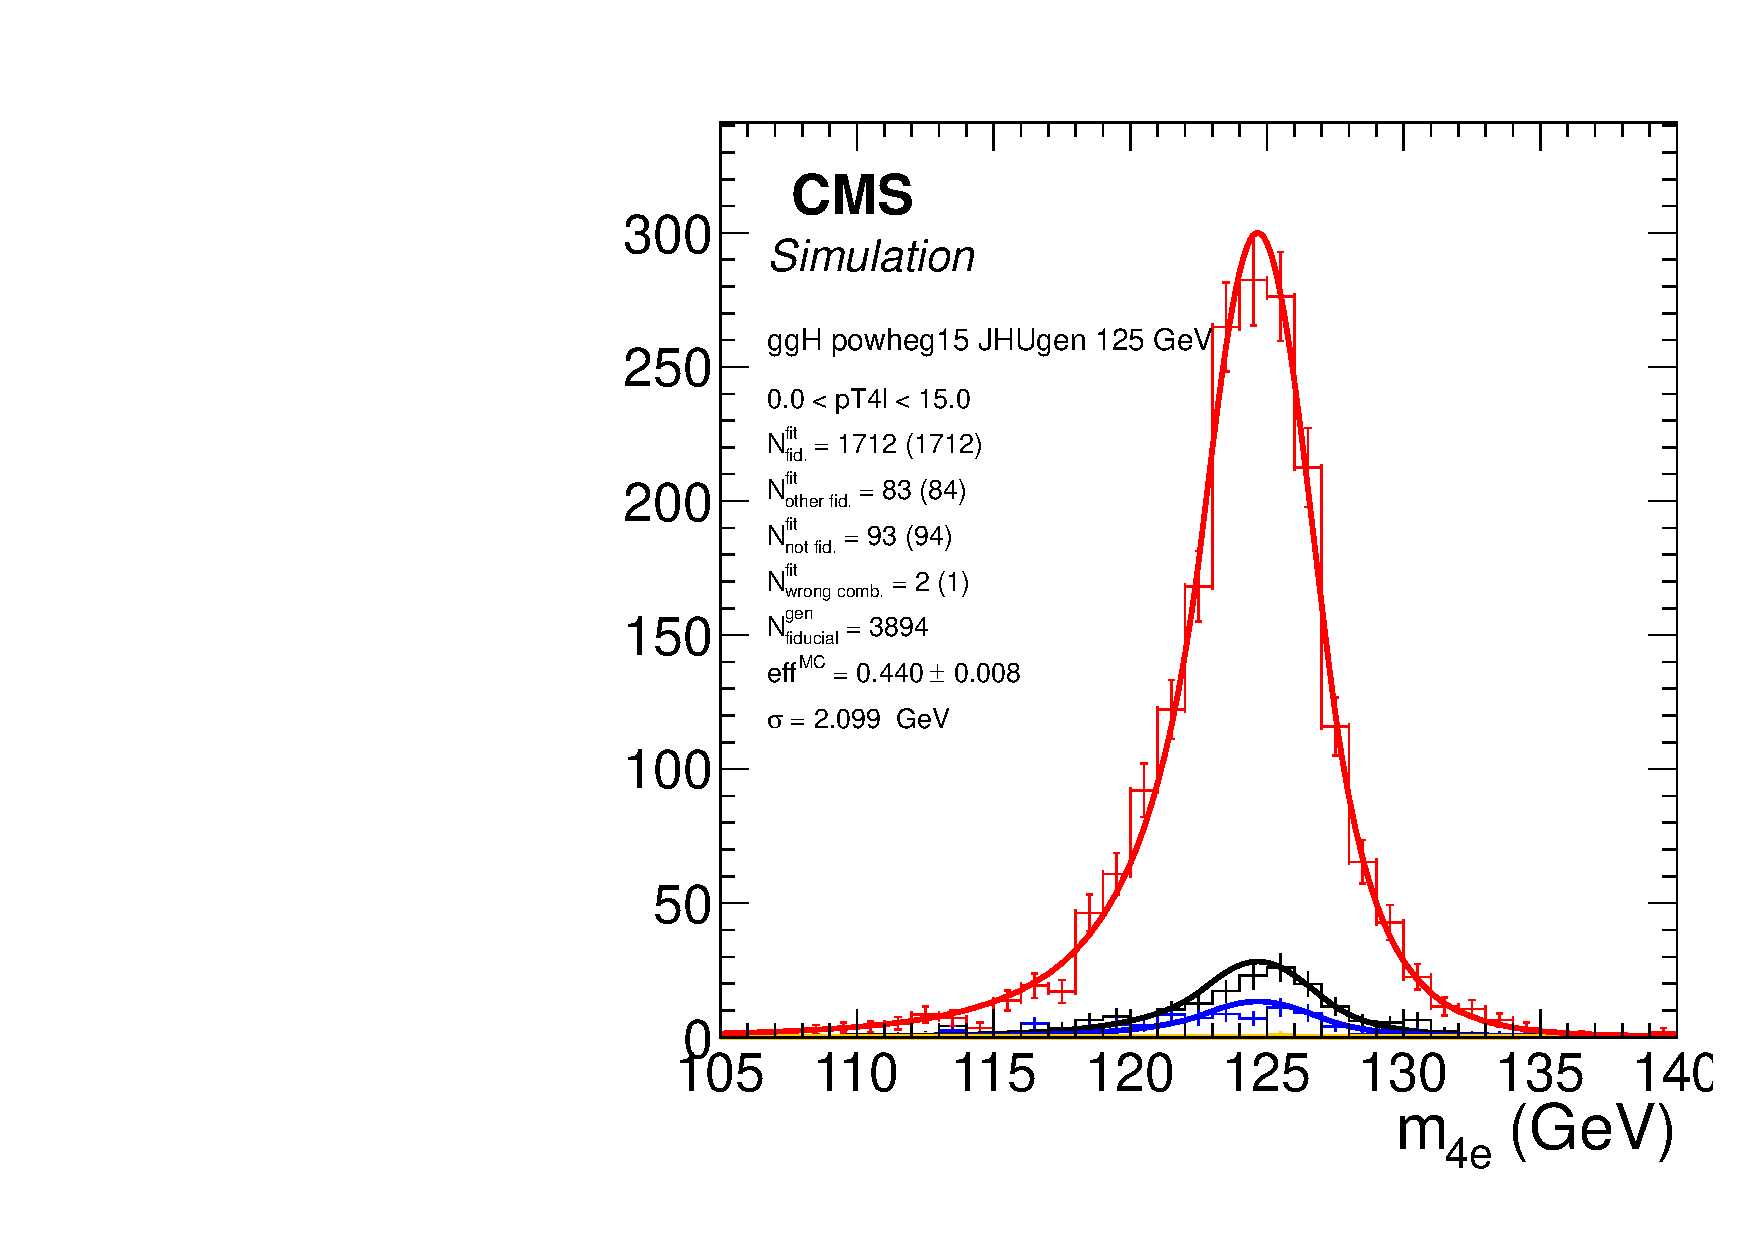
\includegraphics[width=0.3\textwidth,angle=0]{Plots/ggH_powheg15_JHUgen_125_4e_pT4l_genbin0_recobin0_effs_eventMCWeight.pdf}
      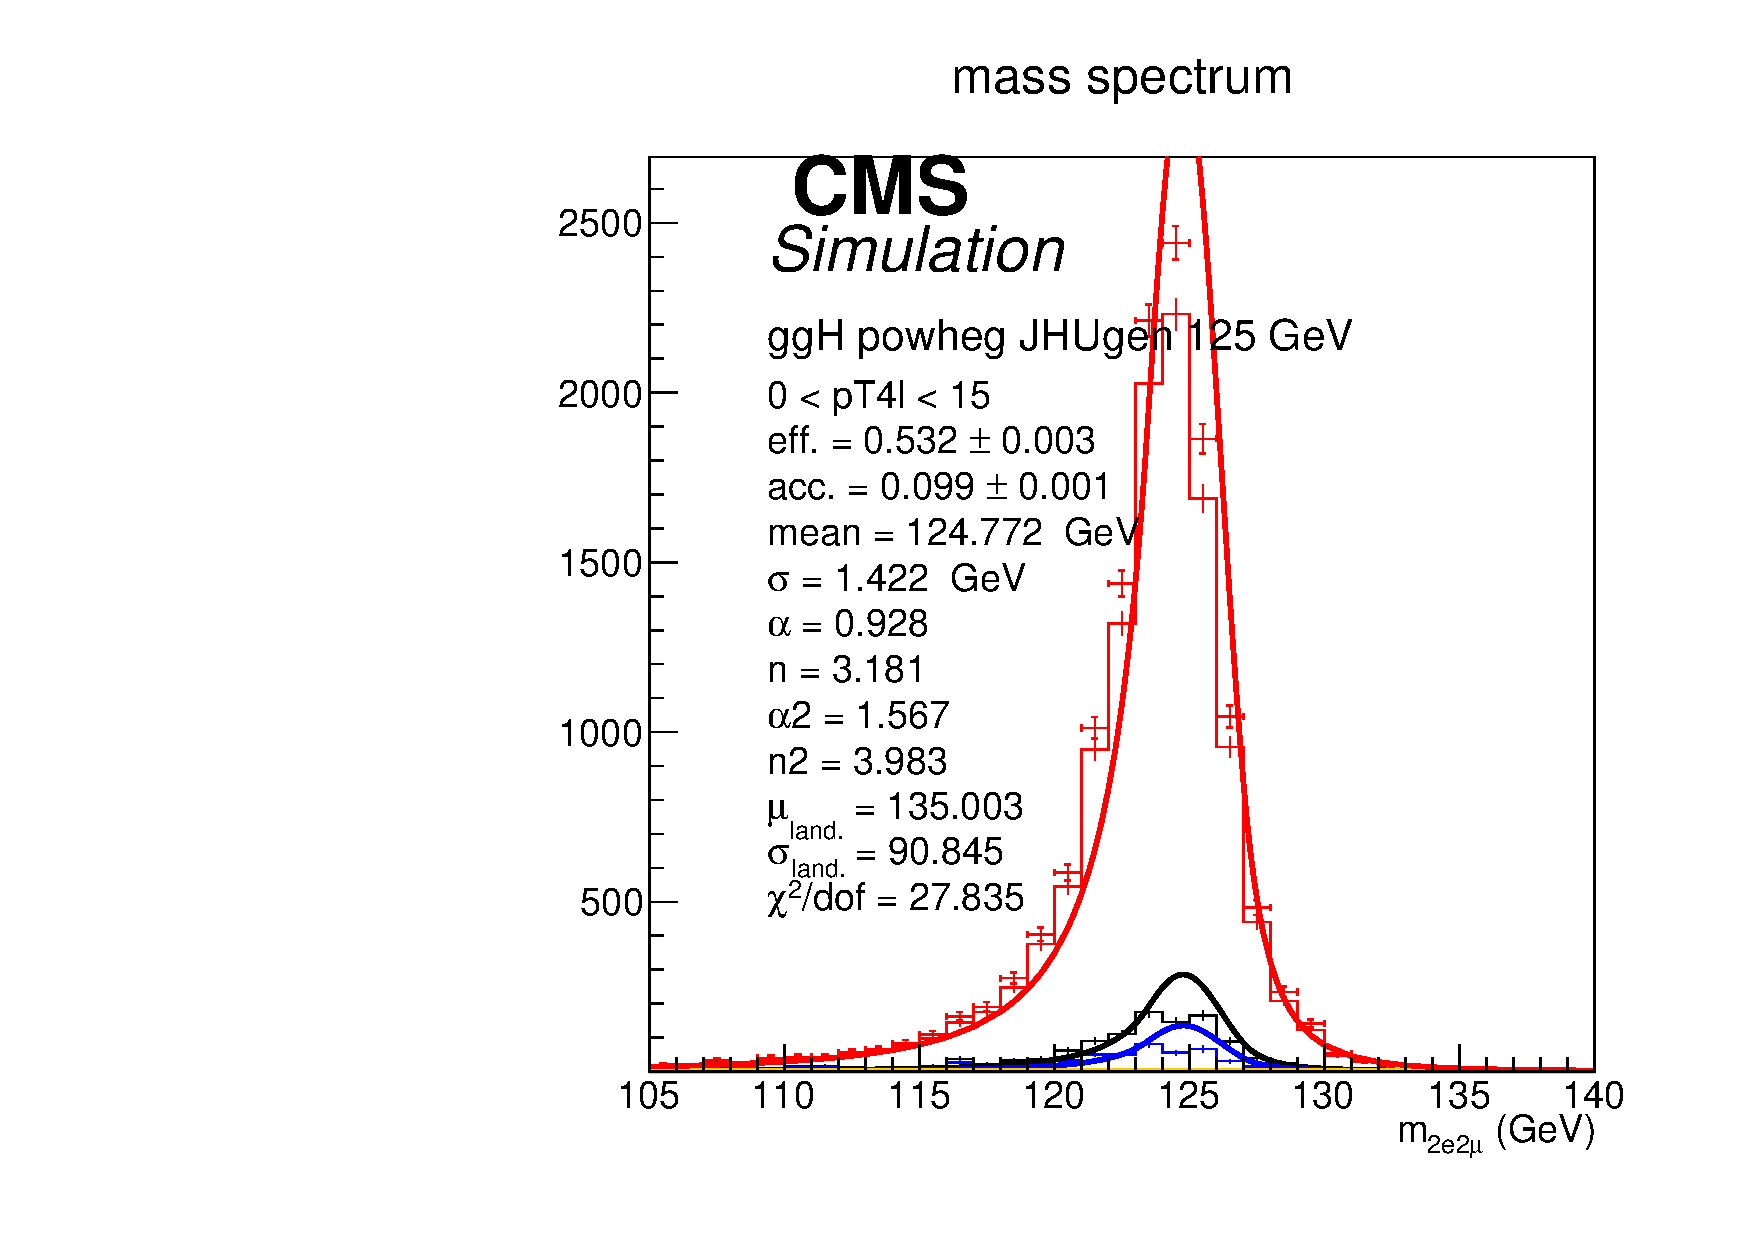
\includegraphics[width=0.3\textwidth,angle=0]{Plots/ggH_powheg_JHUgen_125_2e2mu_pT4l_genbin0_recobin0_effs_genWeight*pileupWeight*dataMCWeight.pdf}
      \label{fig:sigfits-pT4l-ggH-powheg15-JHUgen-125-maintext:a}
    }
    \subfigure[$15.0 < \pt(\mathrm{H}) < 30.0$]{
      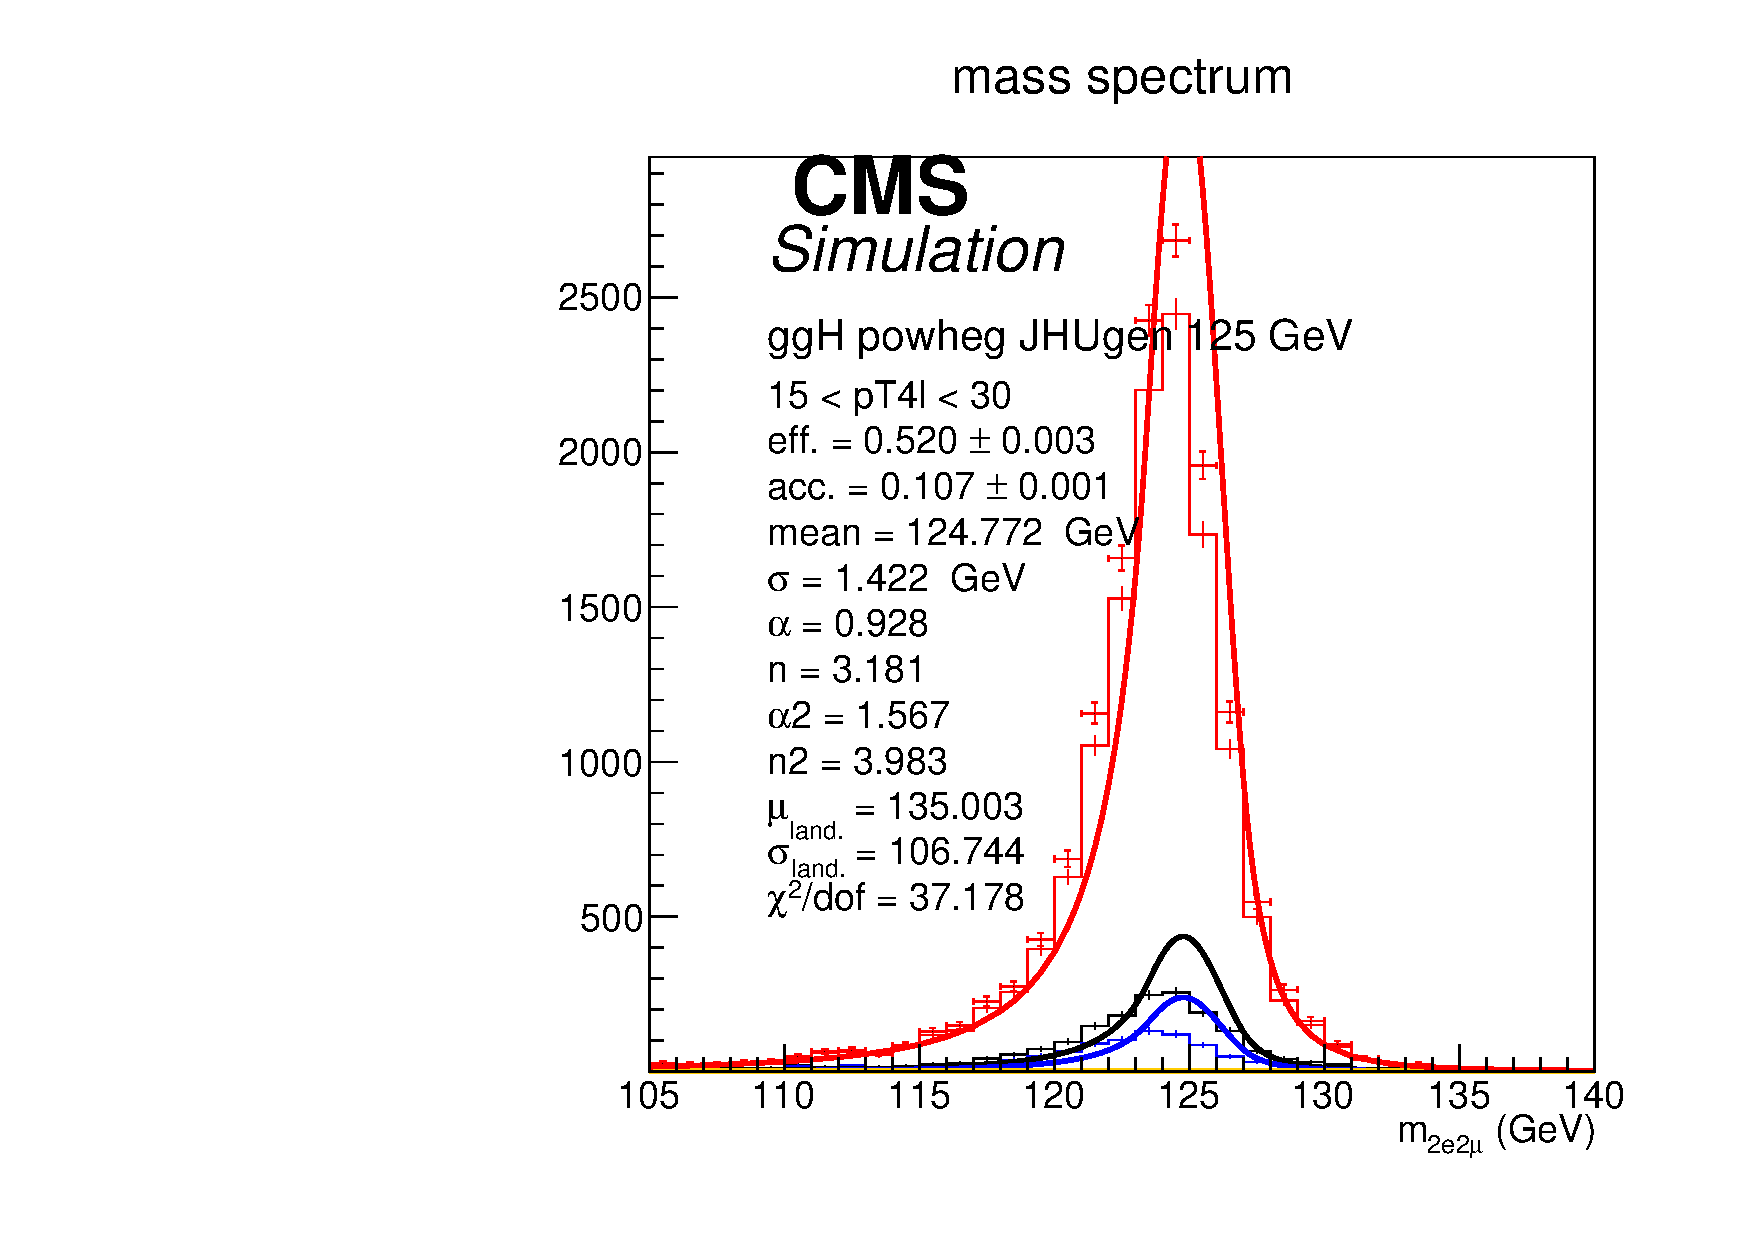
\includegraphics[width=0.3\textwidth,angle=0]{Plots/ggH_powheg_JHUgen_125_2e2mu_pT4l_genbin1_recobin1_effs_genWeight*pileupWeight*dataMCWeight.pdf}
      \label{fig:sigfits-pT4l-ggH-powheg15-JHUgen-125-maintext:b}
    }
   \subfigure[$30.0 < \pt(\mathrm{H}) < 45.0$]{
      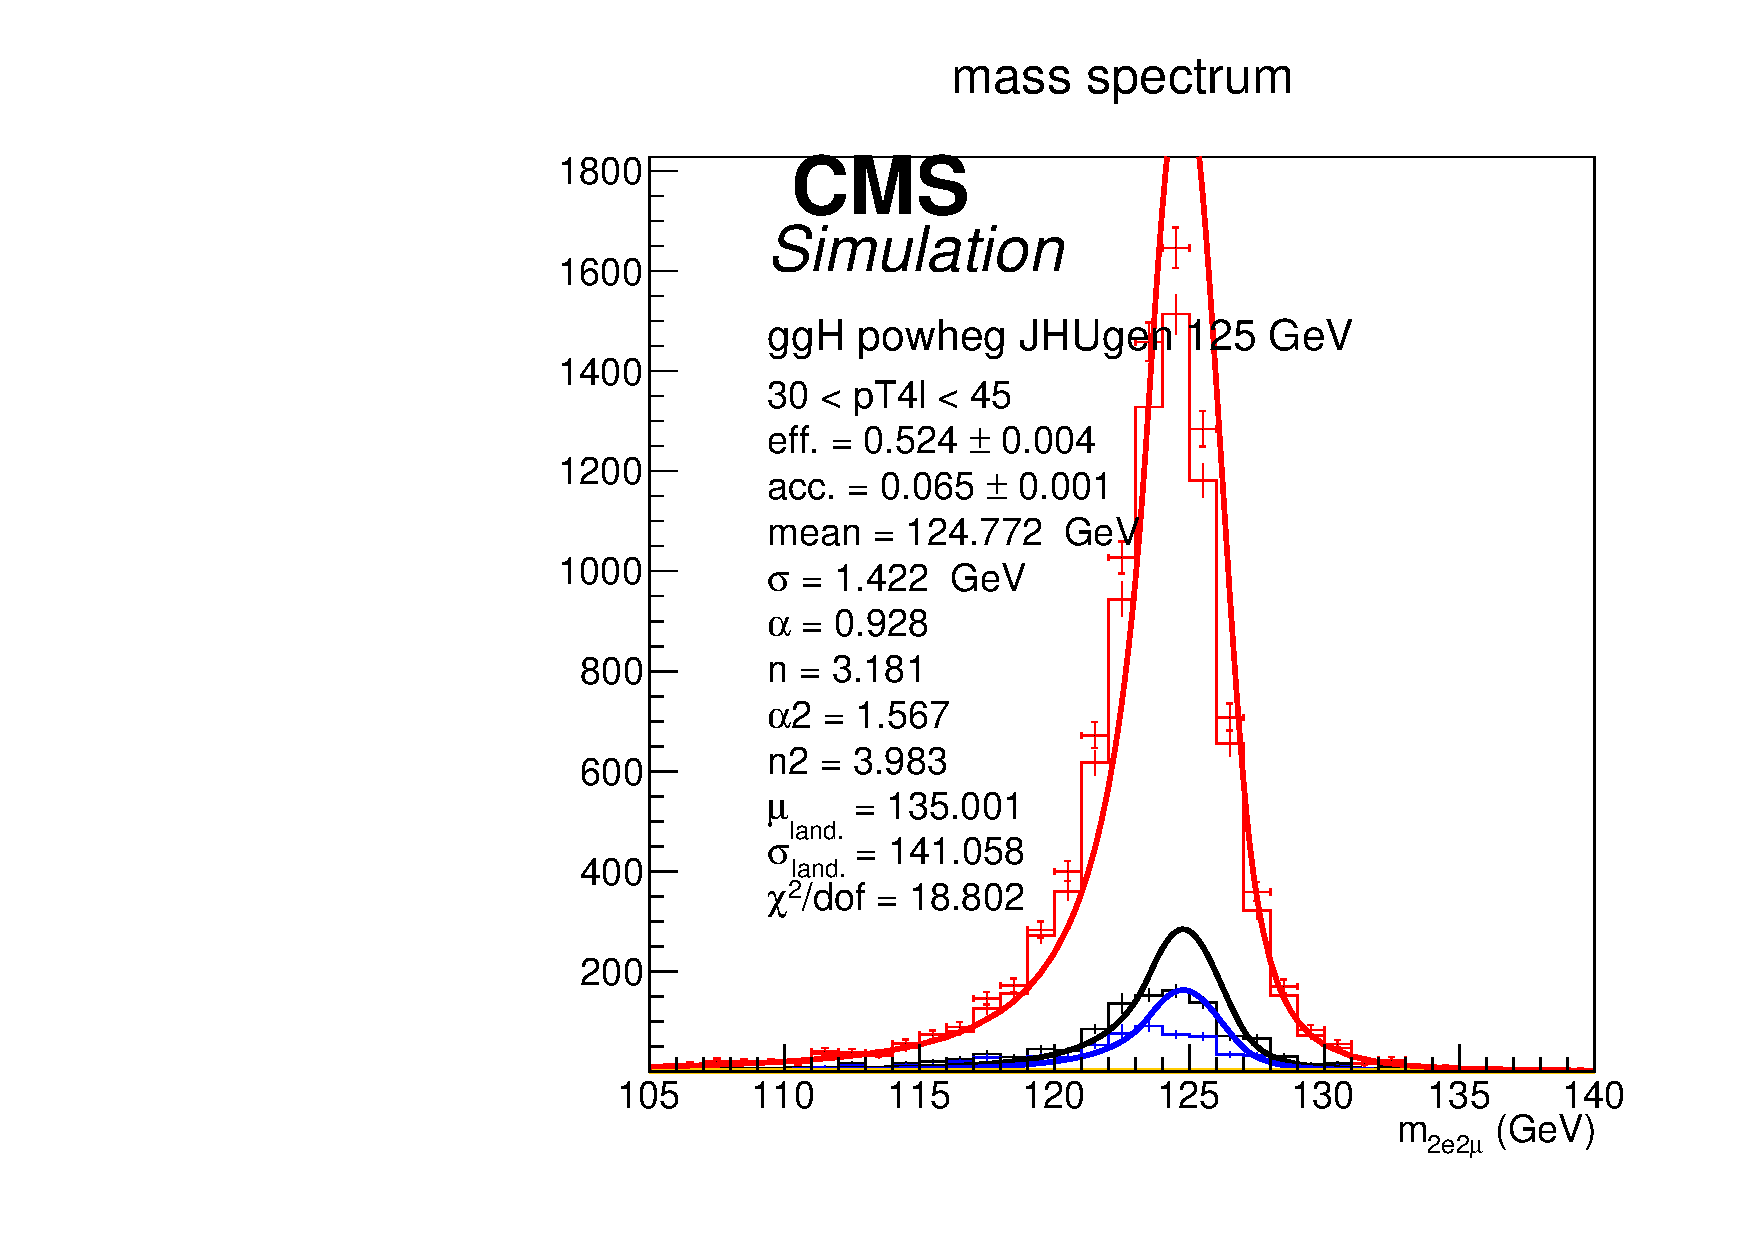
\includegraphics[width=0.3\textwidth,angle=0]{Plots/ggH_powheg_JHUgen_125_2e2mu_pT4l_genbin2_recobin2_effs_genWeight*pileupWeight*dataMCWeight.pdf}
      \label{fig:sigfits-pT4l-ggH-powheg15-JHUgen-125-maintext:c}
    }  \\
    \subfigure[$45.0 < \pt(\mathrm{H}) < 80.0$]{
      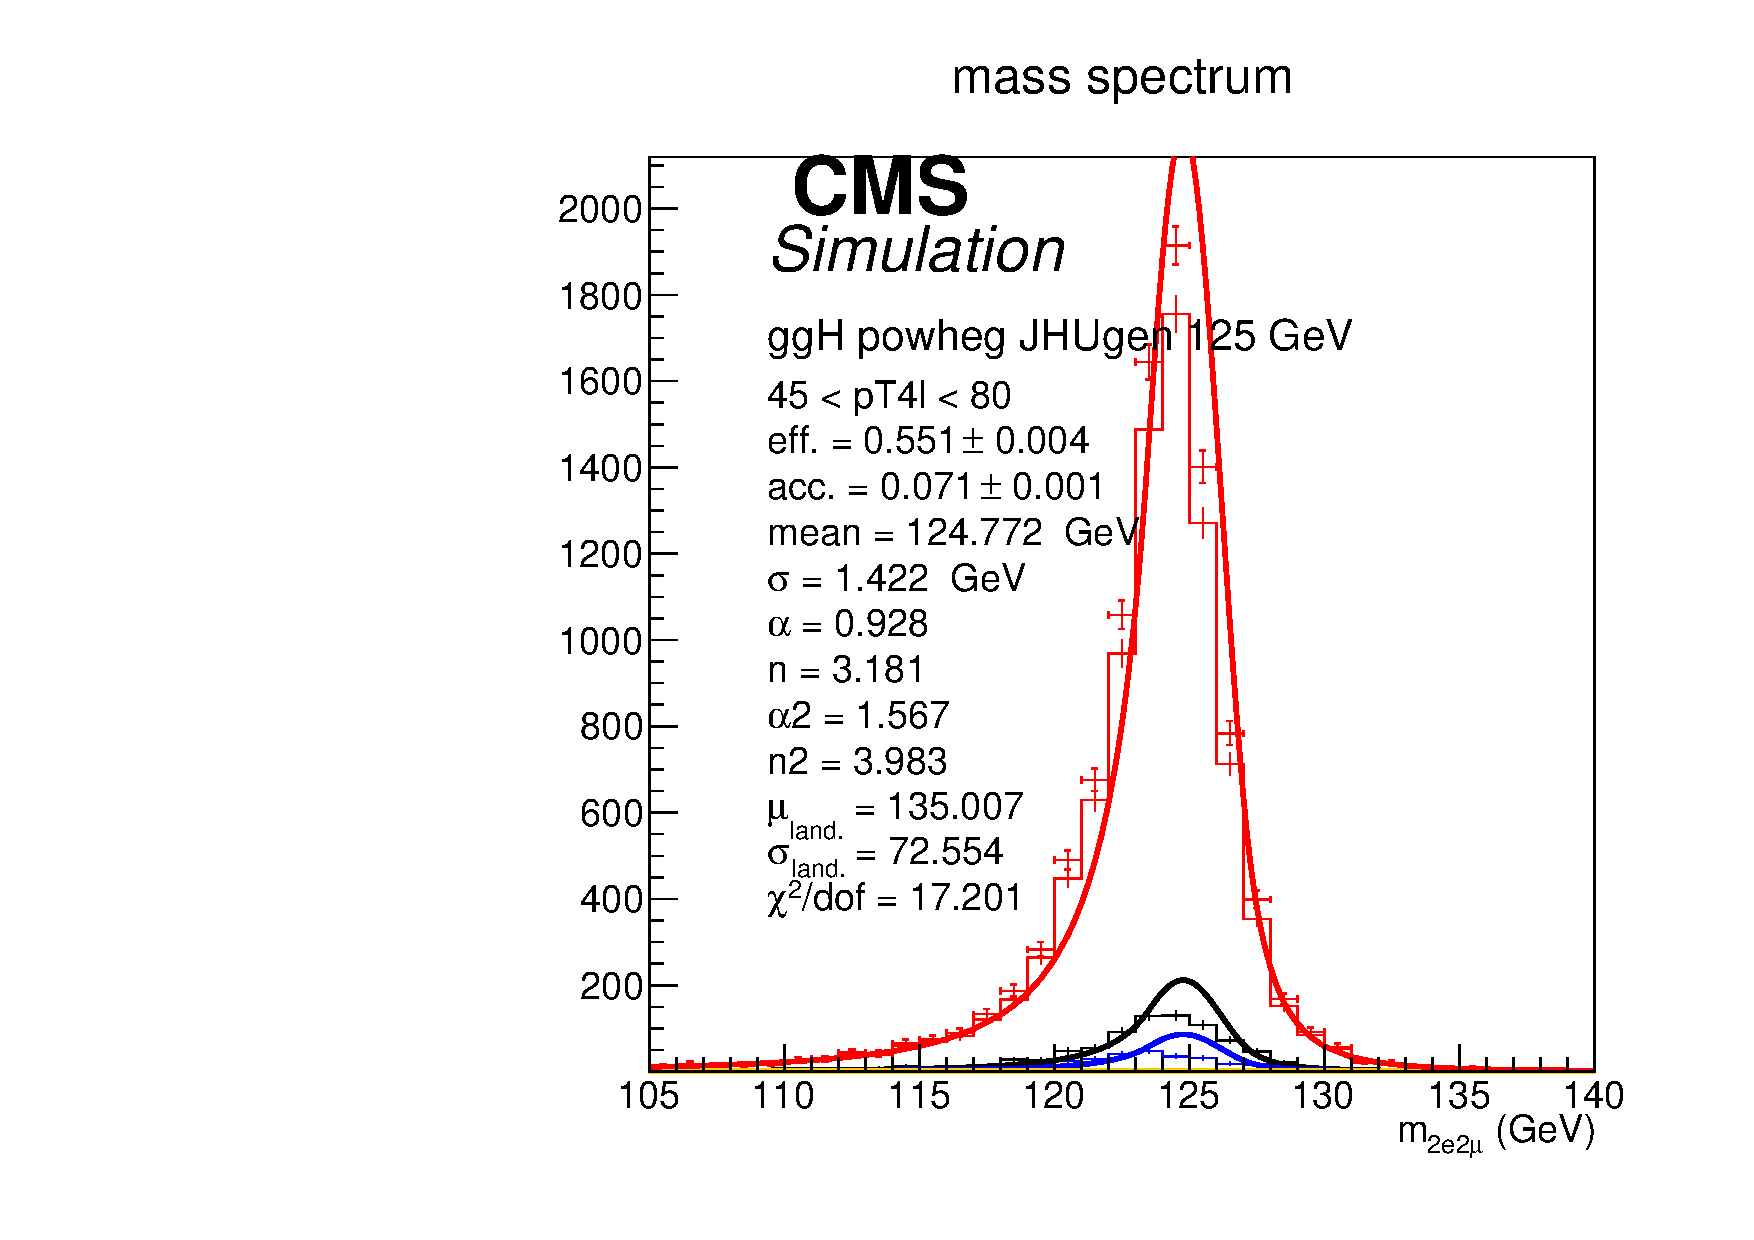
\includegraphics[width=0.3\textwidth,angle=0]{Plots/ggH_powheg_JHUgen_125_2e2mu_pT4l_genbin3_recobin3_effs_genWeight*pileupWeight*dataMCWeight.pdf}
      \label{fig:sigfits-pT4l-ggH-powheg15-JHUgen-125-maintext:d}
    }
    \subfigure[$80.0 < \pt(\mathrm{H}) < 120.0$]{
      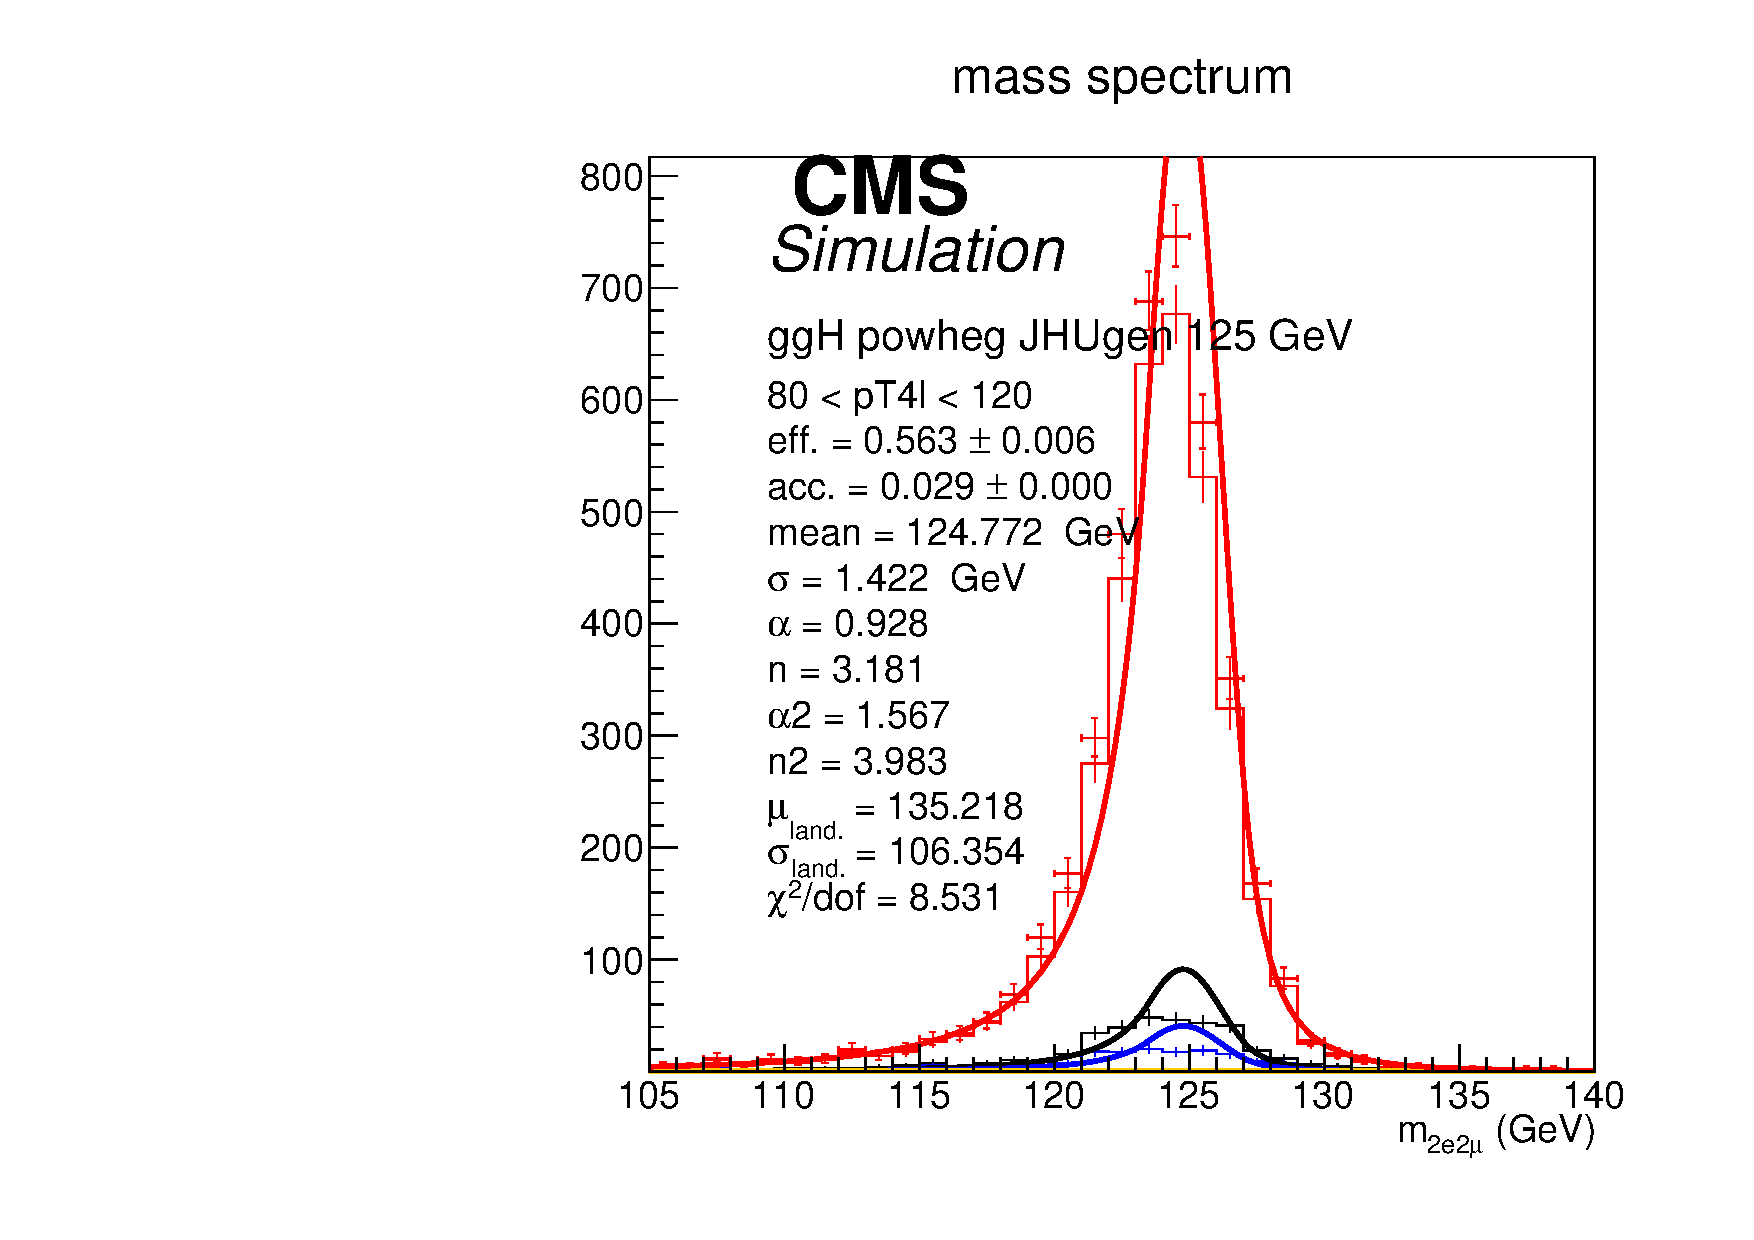
\includegraphics[width=0.3\textwidth,angle=0]{Plots/ggH_powheg_JHUgen_125_2e2mu_pT4l_genbin4_recobin4_effs_genWeight*pileupWeight*dataMCWeight.pdf}
      \label{fig:sigfits-pT4l-ggH-powheg15-JHUgen-125-maintext:e}
    }
    \subfigure[$120.0 < \pt(\mathrm{H}) < 200.0$]{
      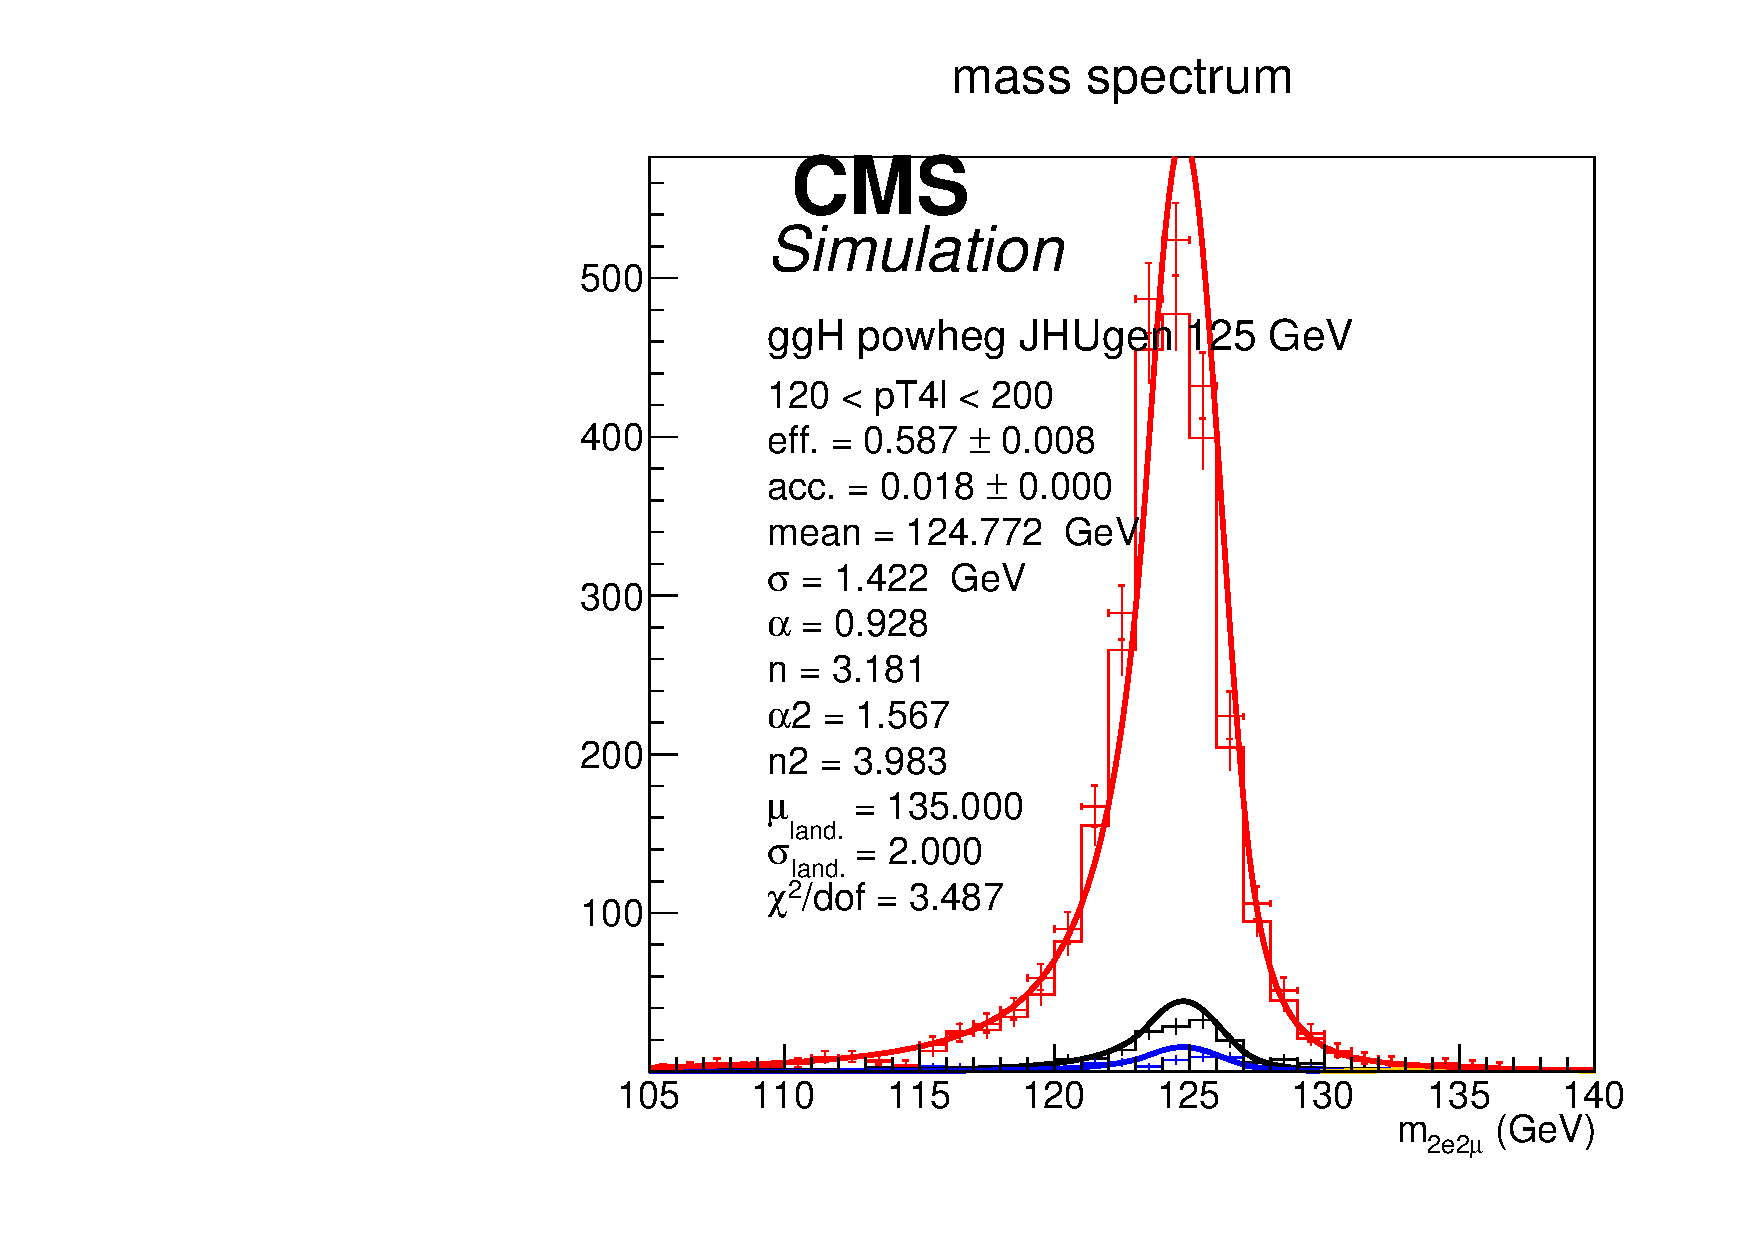
\includegraphics[width=0.3\textwidth,angle=0]{Plots/ggH_powheg_JHUgen_125_2e2mu_pT4l_genbin5_recobin5_effs_genWeight*pileupWeight*dataMCWeight.pdf}
      \label{fig:sigfits-pT4l-ggH-powheg15-JHUgen-125-maintext:f}
    } \\
    \subfigure[$200.0 < \pt(\mathrm{H}) < 13000.0$]{
      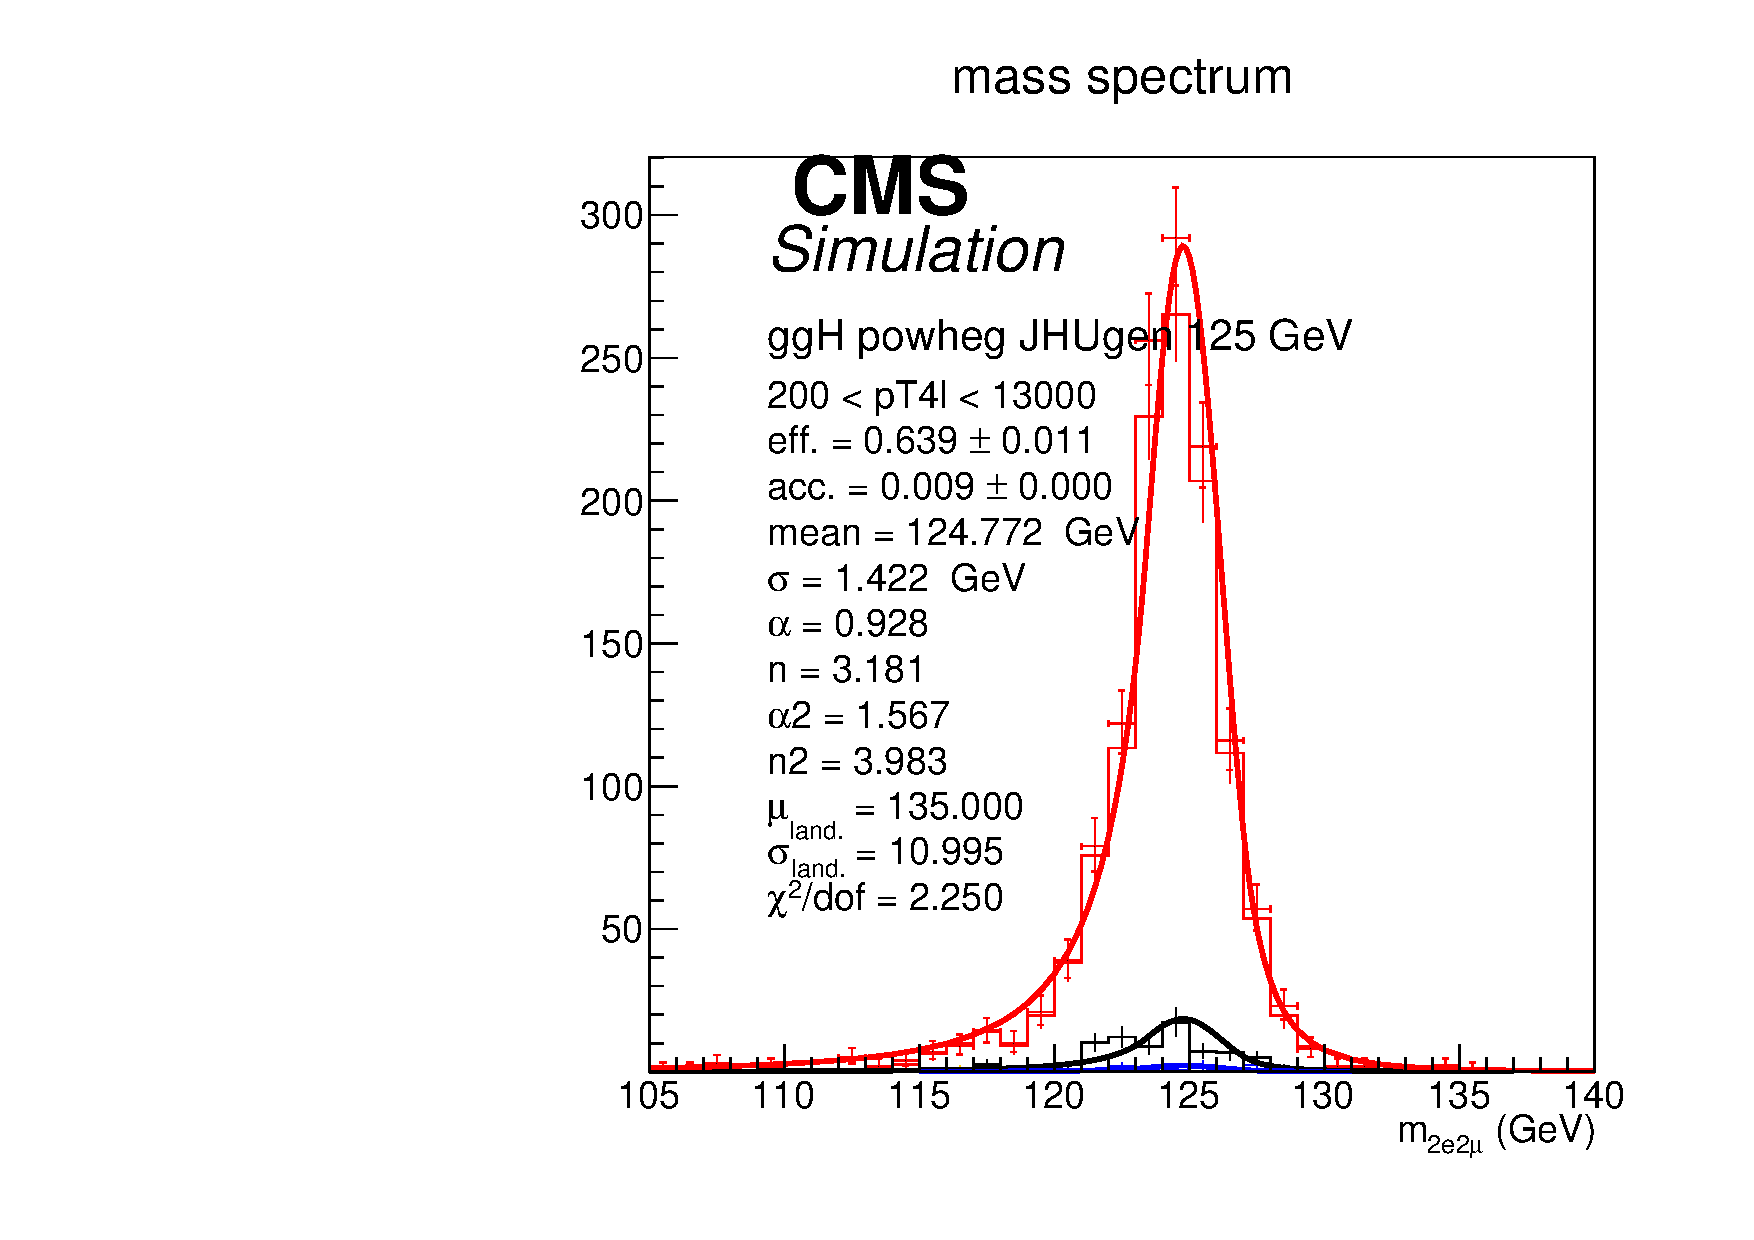
\includegraphics[width=0.3\textwidth,angle=0]{Plots/ggH_powheg_JHUgen_125_2e2mu_pT4l_genbin6_recobin6_effs_genWeight*pileupWeight*dataMCWeight.pdf}
      \label{fig:sigfits-pT4l-ggH-powheg15-JHUgen-125-maintext:g}
    }
%    \subfigure[$30.0 < \pt(\mathrm{H}) < 60.0$]{
%      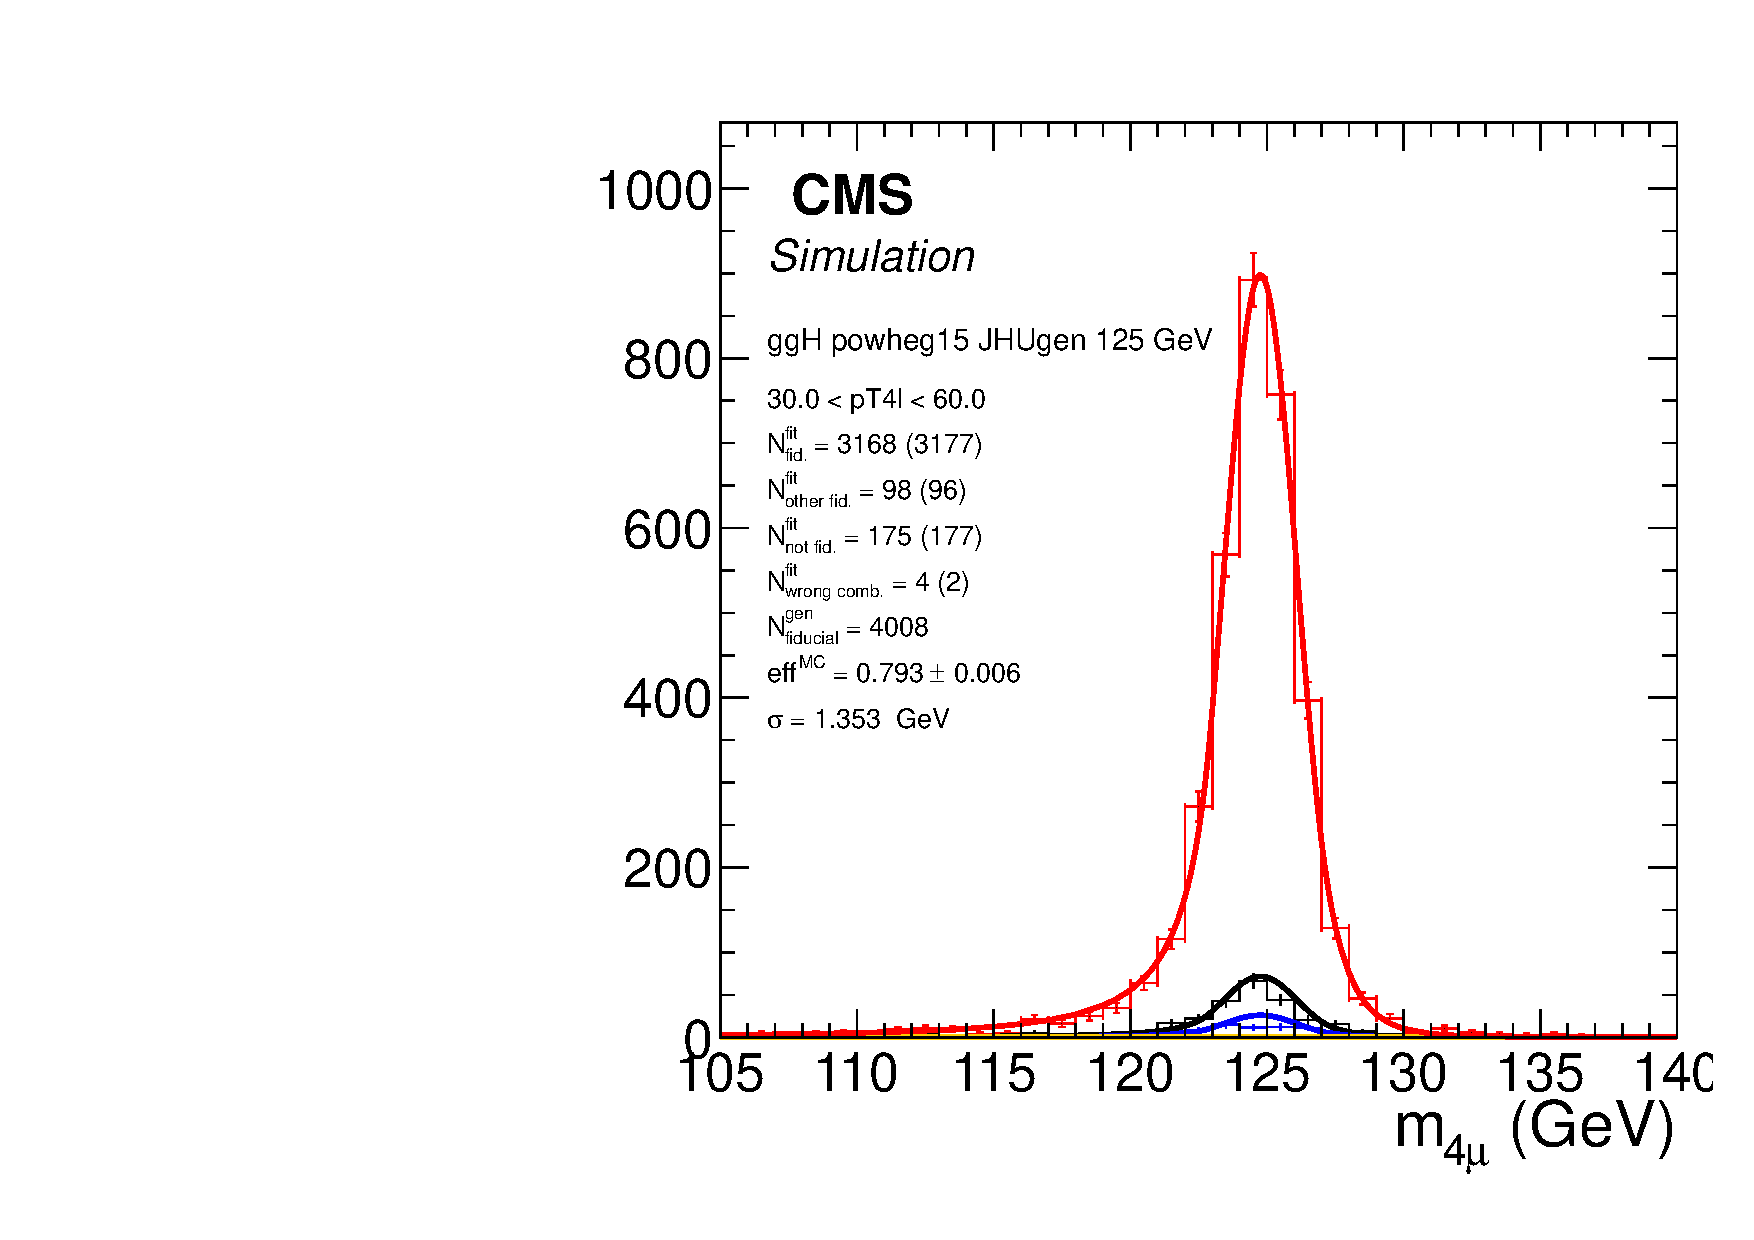
\includegraphics[width=0.3\textwidth,angle=0]{Plots/ggH_powheg15_JHUgen_125_4mu_pT4l_genbin2_recobin2_effs_eventMCWeight.pdf}
%      \label{fig:sigfits-pT4l-ggH-powheg15-JHUgen-125-maintext:h}
%    }
%    \subfigure[$30.0  < \pt(\mathrm{H}) < 60.0$]{
%      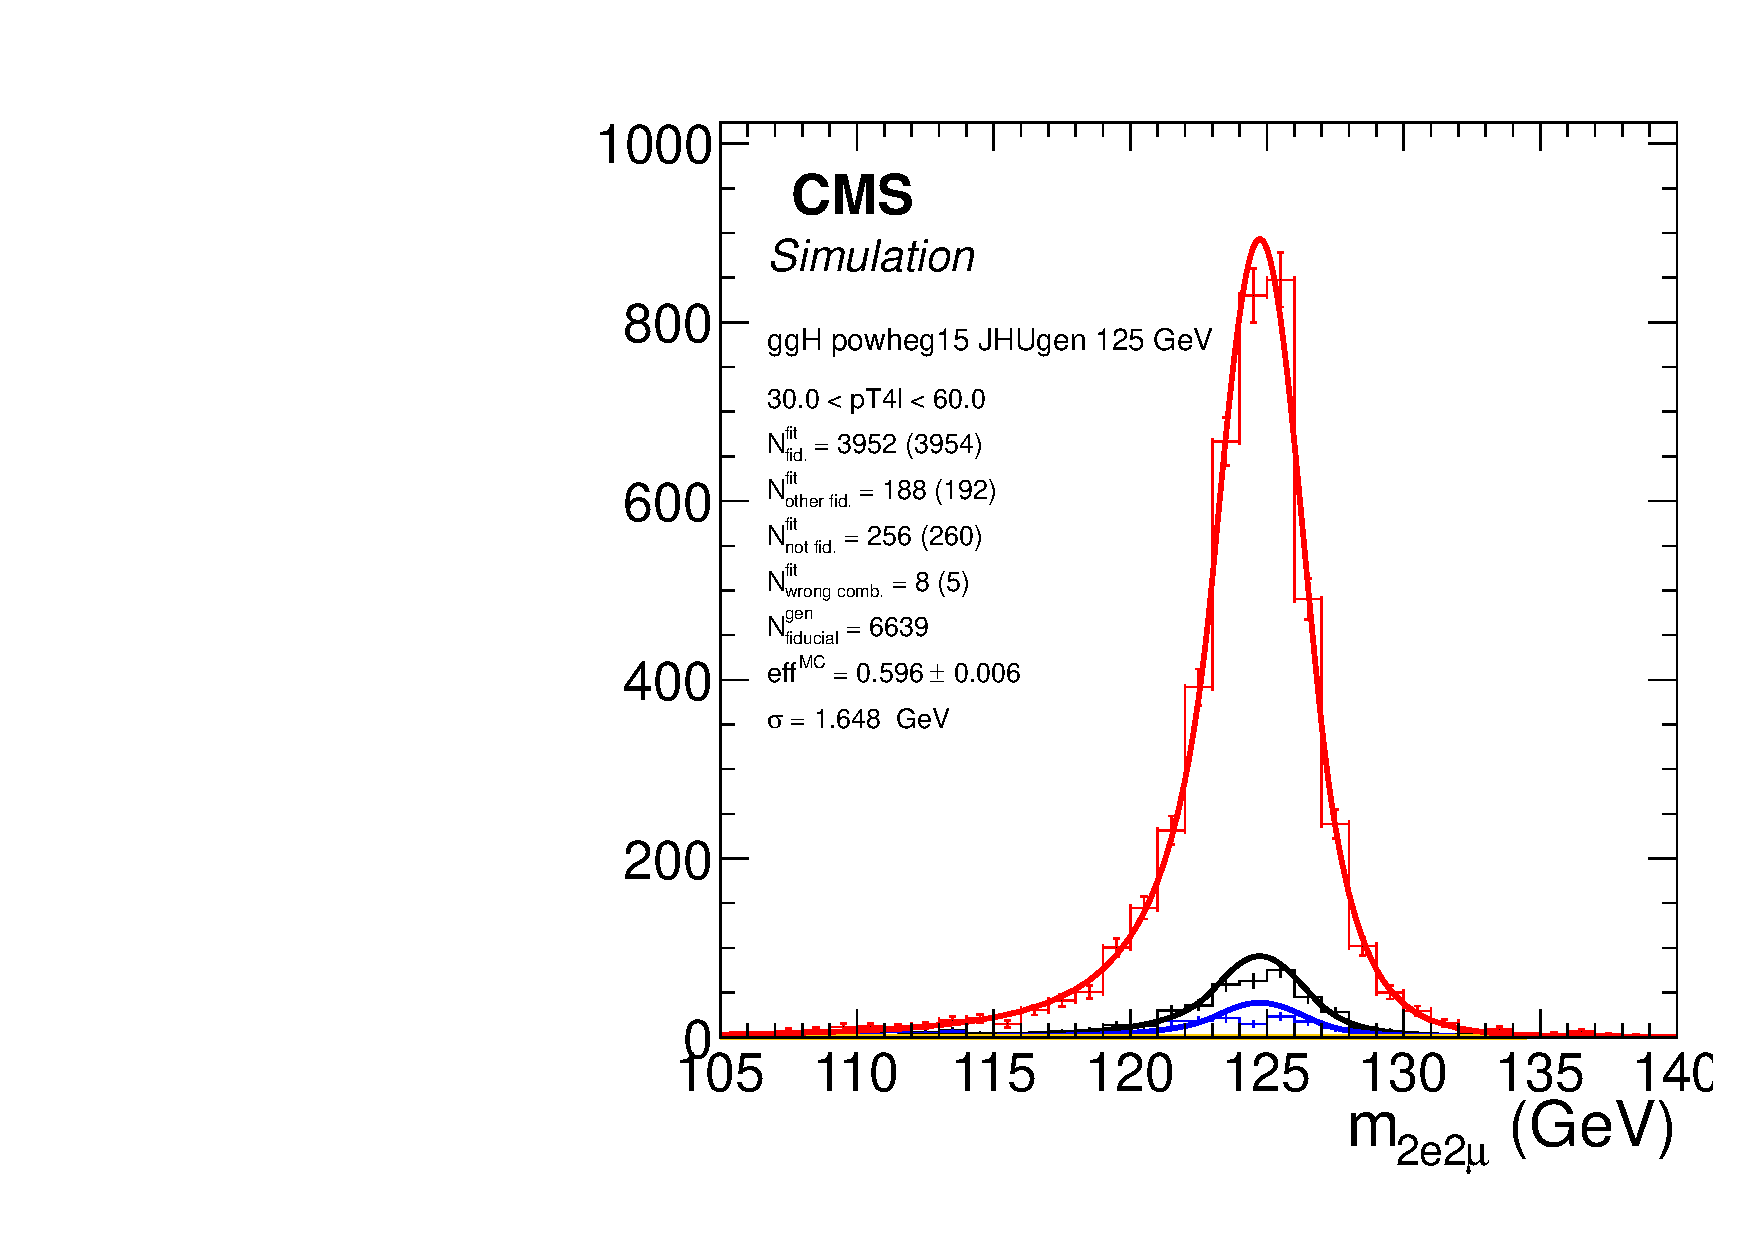
\includegraphics[width=0.3\textwidth,angle=0]{Plots/ggH_powheg15_JHUgen_125_2e2mu_pT4l_genbin2_recobin2_effs_eventMCWeight.pdf}
%      \label{fig:sigfits-pT4l-ggH-powheg15-JHUgen-125-maintext:i}
%    } \\
%    \subfigure[$60.0  < \pt(\mathrm{H}) < 200.0 $]{
%      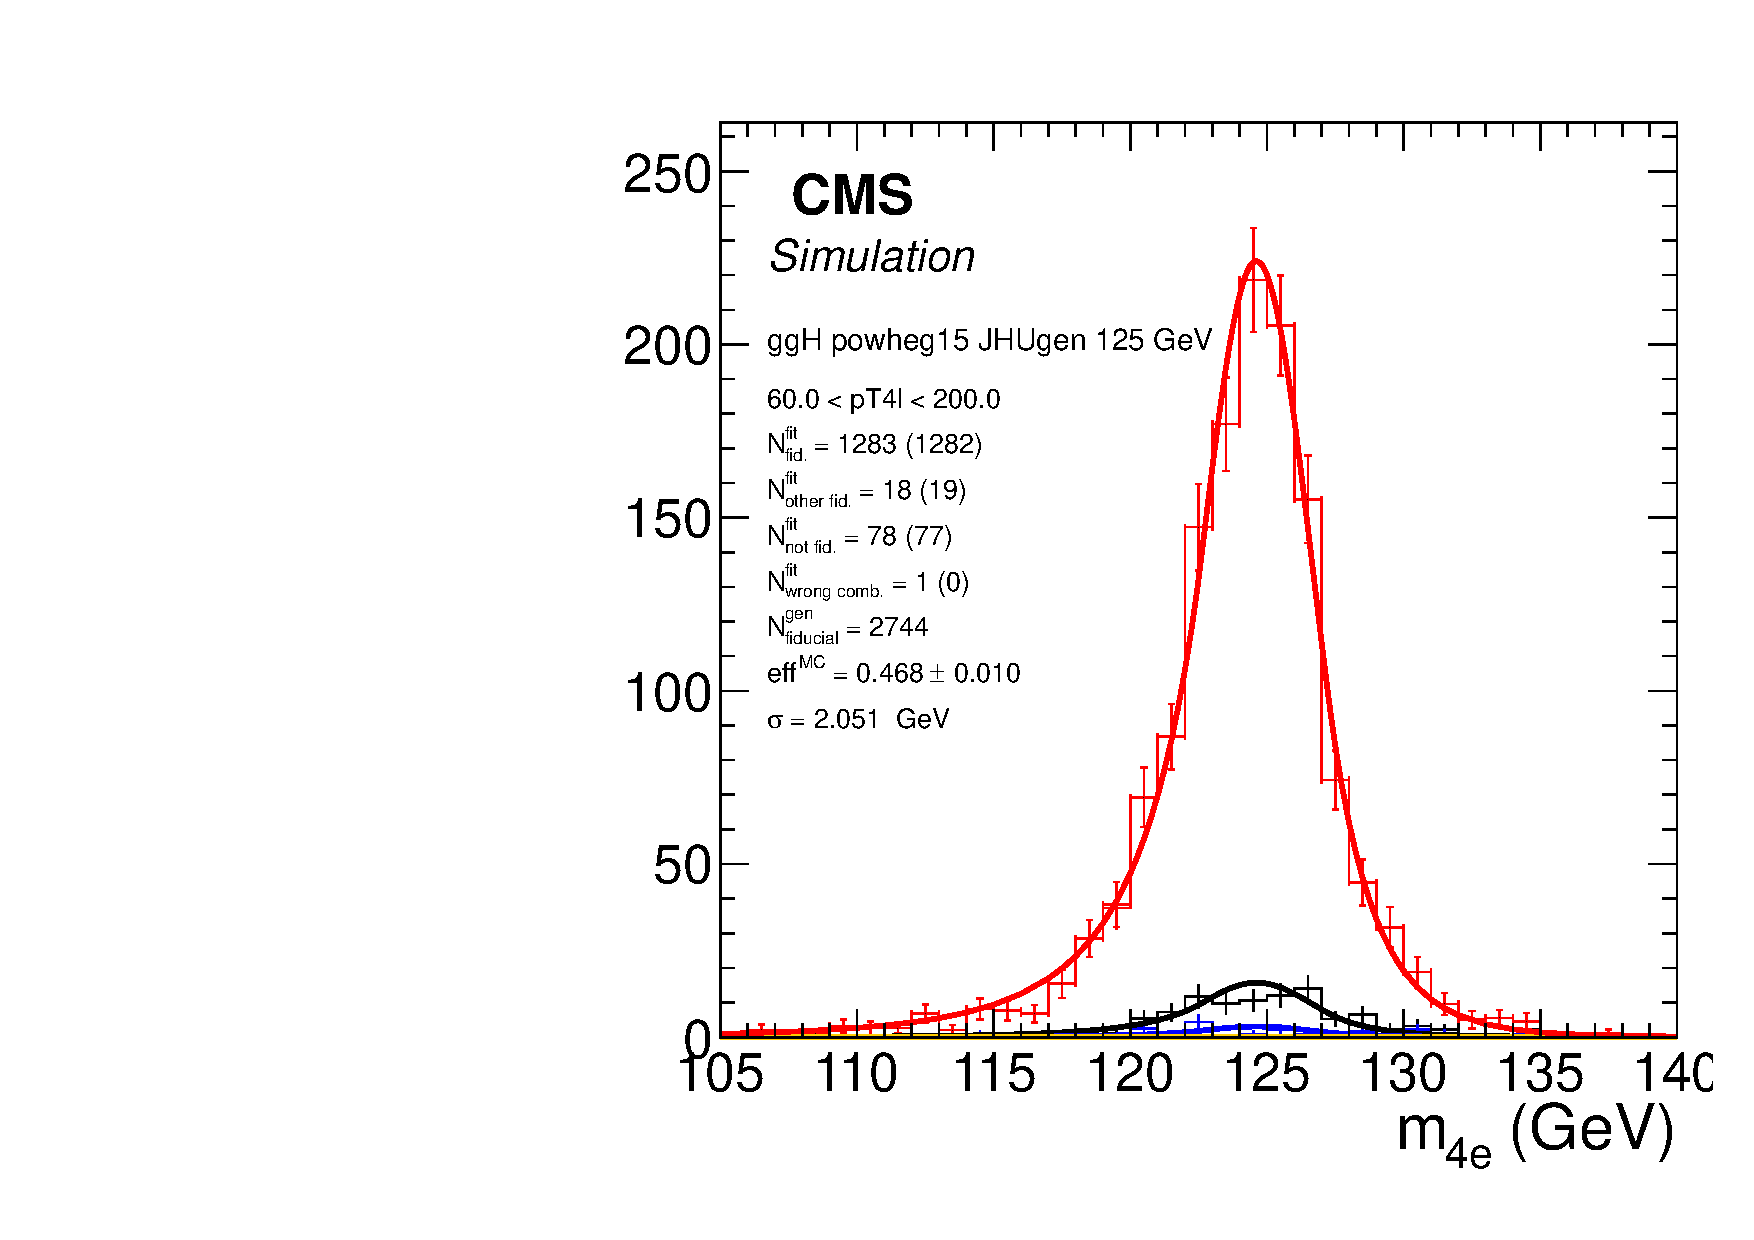
\includegraphics[width=0.3\textwidth,angle=0]{Plots/ggH_powheg15_JHUgen_125_4e_pT4l_genbin3_recobin3_effs_eventMCWeight.pdf}
%      \label{fig:sigfits-pT4l-ggH-powheg15-JHUgen-125-maintext:j}
%    }
%    \subfigure[$60.0  < \pt(\mathrm{H}) < 200.0 $]{
%      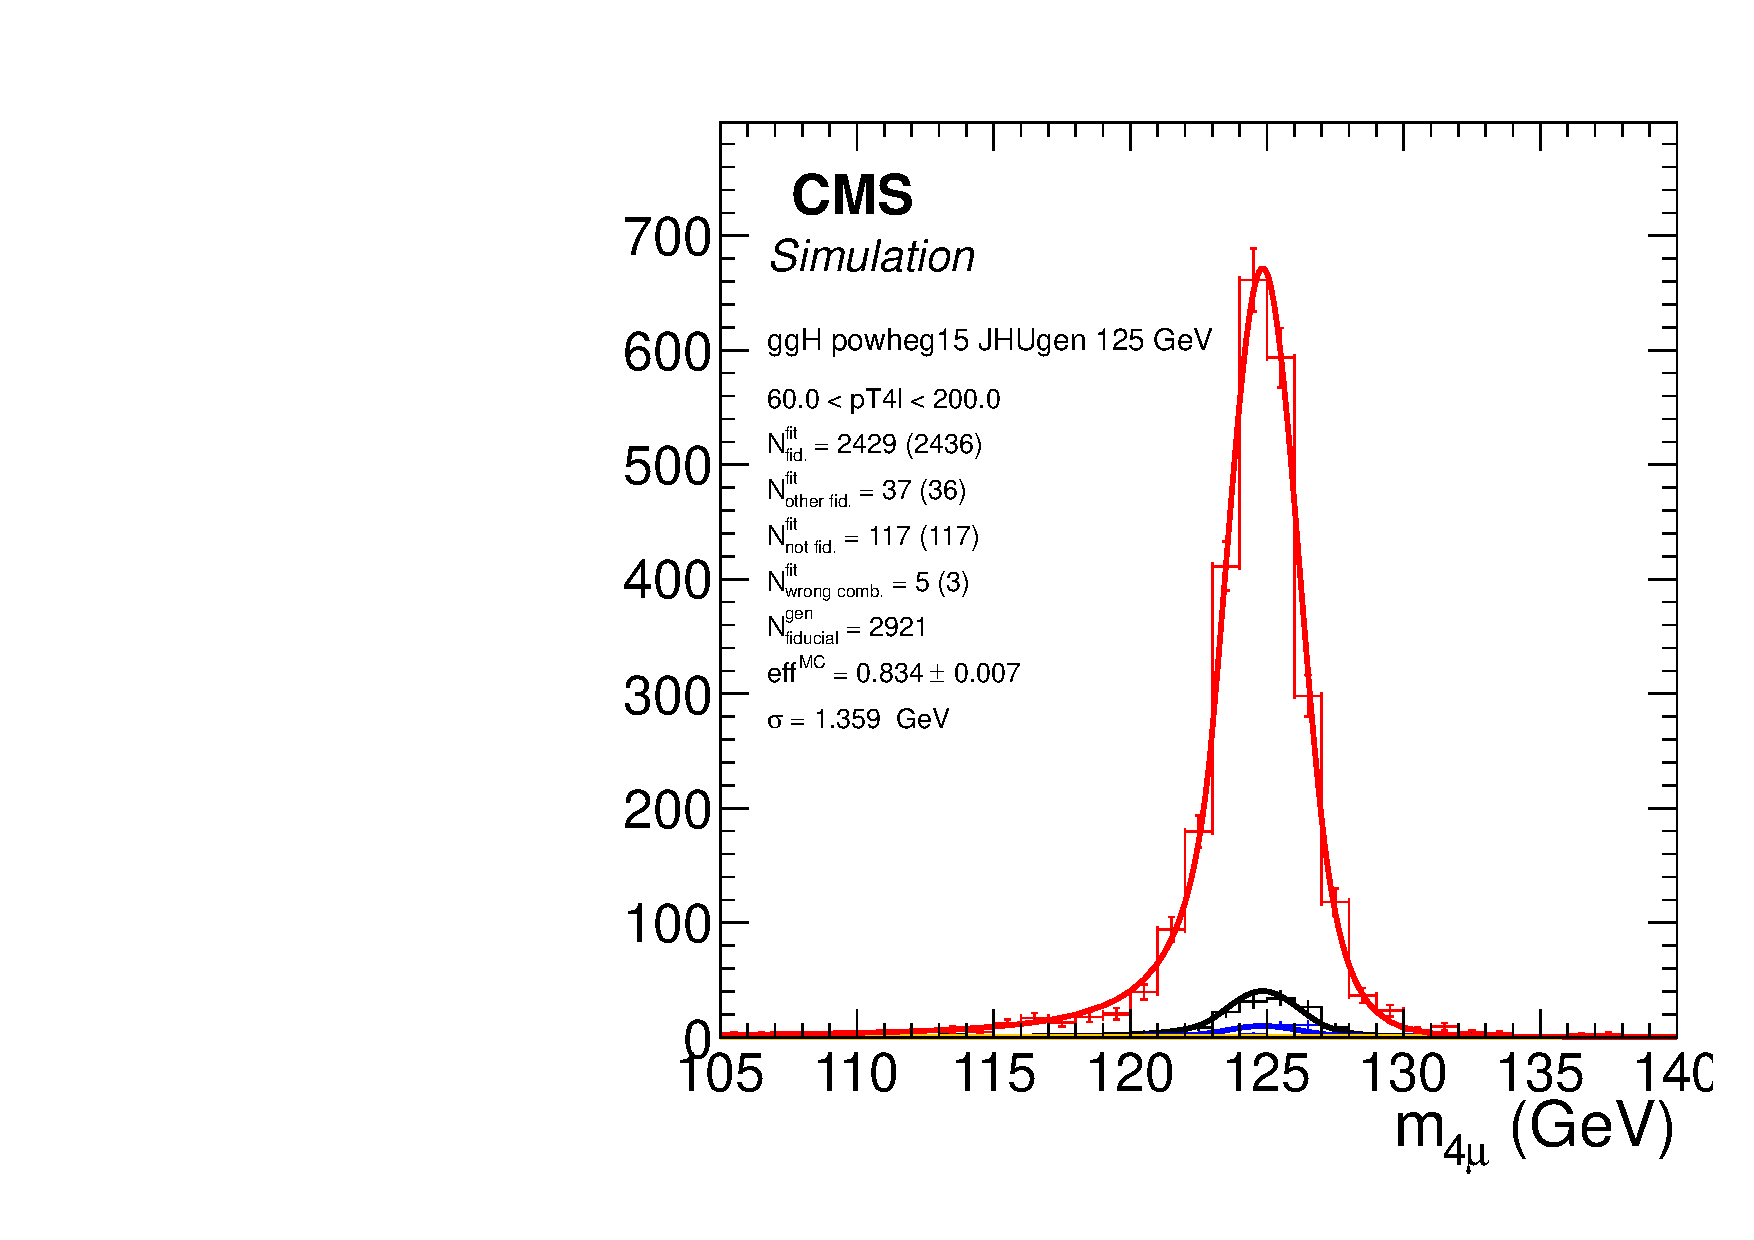
\includegraphics[width=0.3\textwidth,angle=0]{Plots/ggH_powheg15_JHUgen_125_4mu_pT4l_genbin3_recobin3_effs_eventMCWeight.pdf}
%      \label{fig:sigfits-pT4l-ggH-powheg15-JHUgen-125-maintext:k}
%    }
%    \subfigure[$60.0  < \pt(\mathrm{H}) < 200.0$]{
%      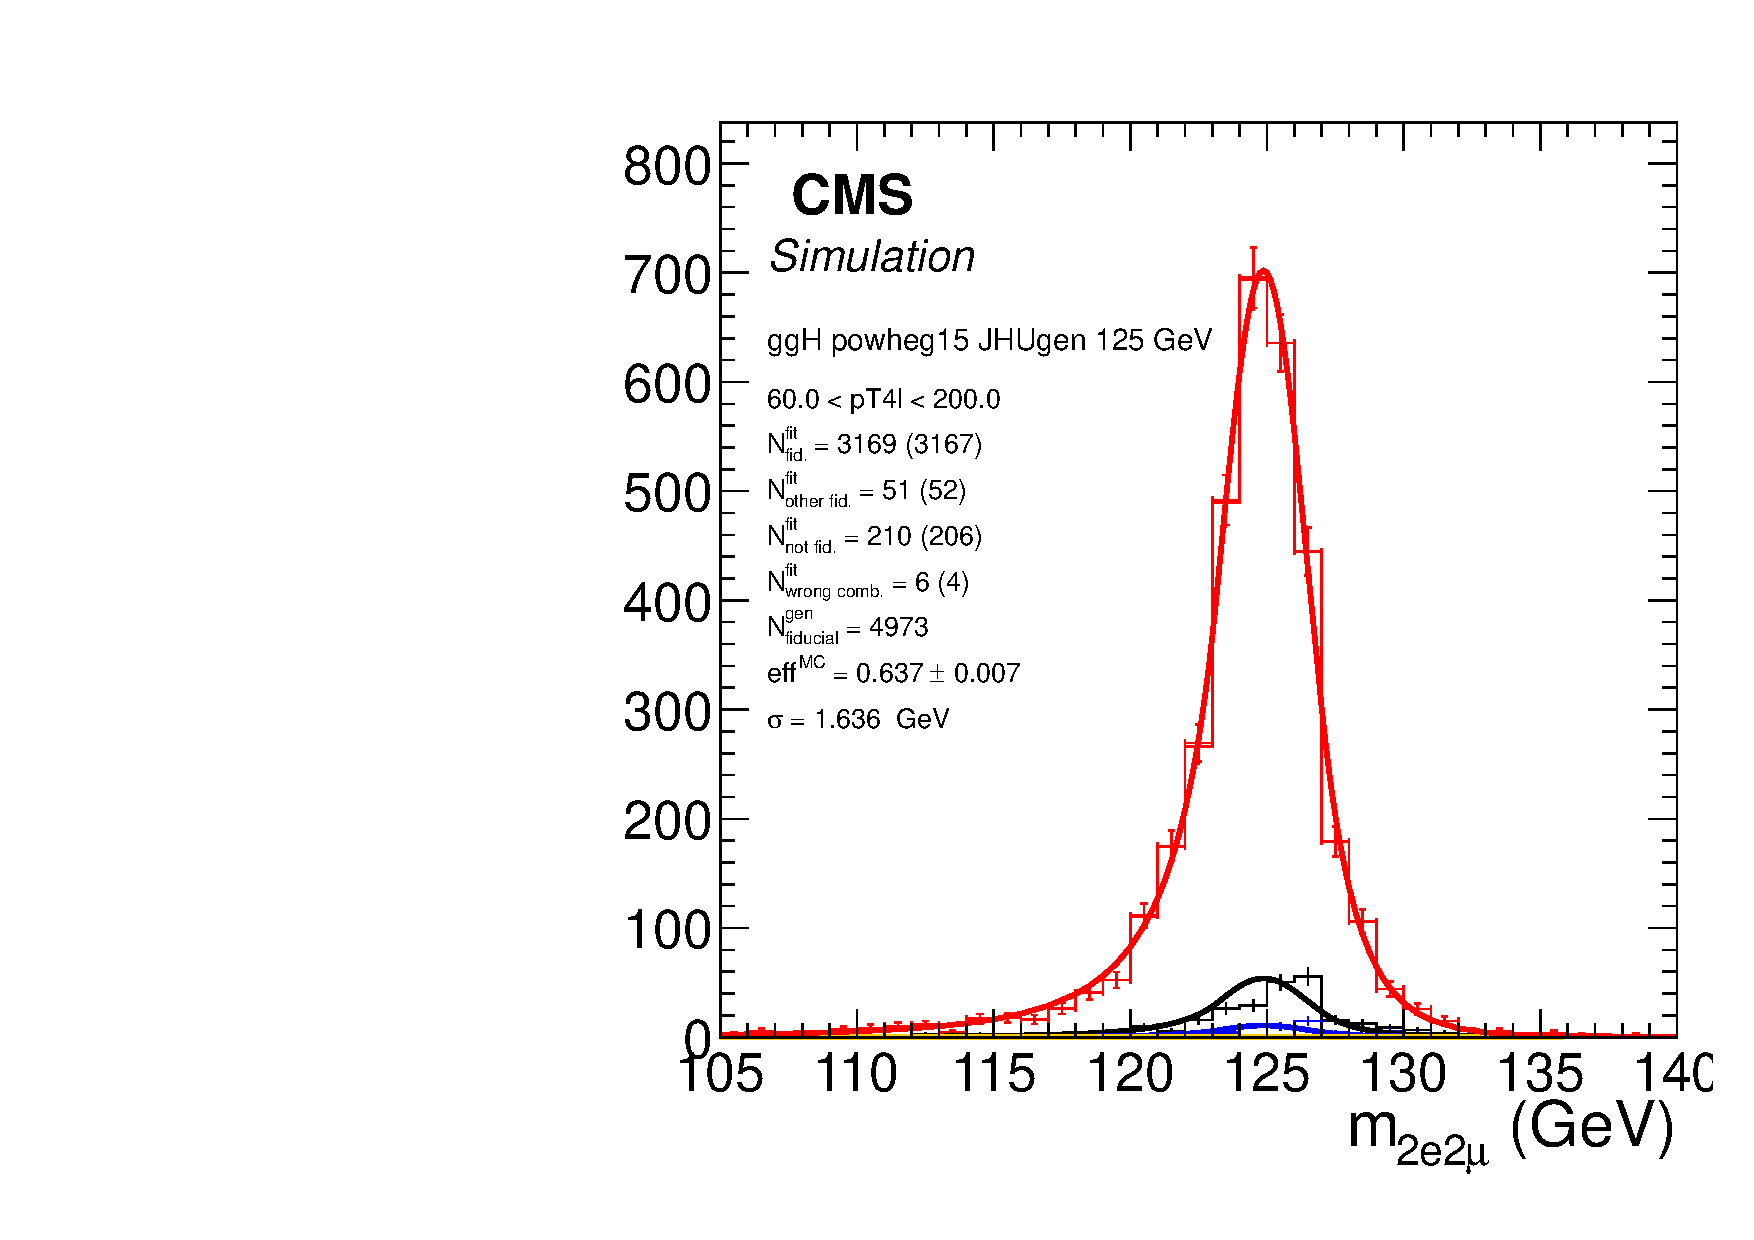
\includegraphics[width=0.3\textwidth,angle=0]{Plots/ggH_powheg15_JHUgen_125_2e2mu_pT4l_genbin3_recobin3_effs_eventMCWeight.pdf}
%      \label{fig:sigfits-pT4l-ggH-powheg15-JHUgen-125-maintext:l}
%    }
    \\
    \caption{ Distributions of m(4$\ell$) in $2e2\mu$ final state for the $gg\rightarrow \mathrm{H}$ production mode from {\sc powheg+JHUGen} in different bins of $\pt(\mathrm{H})$.
    }
  \label{fig:sigfits-pT4l-ggH-powheg15-JHUgen-125-maintext}
 \end{center}
\end{figure} \clearpage

%%%%%%%%%5
\begin{figure}[htb]
  \begin{center}
    \subfigure[$gg\rightarrow$H ({\sc powheg+JHUgen})]{
    %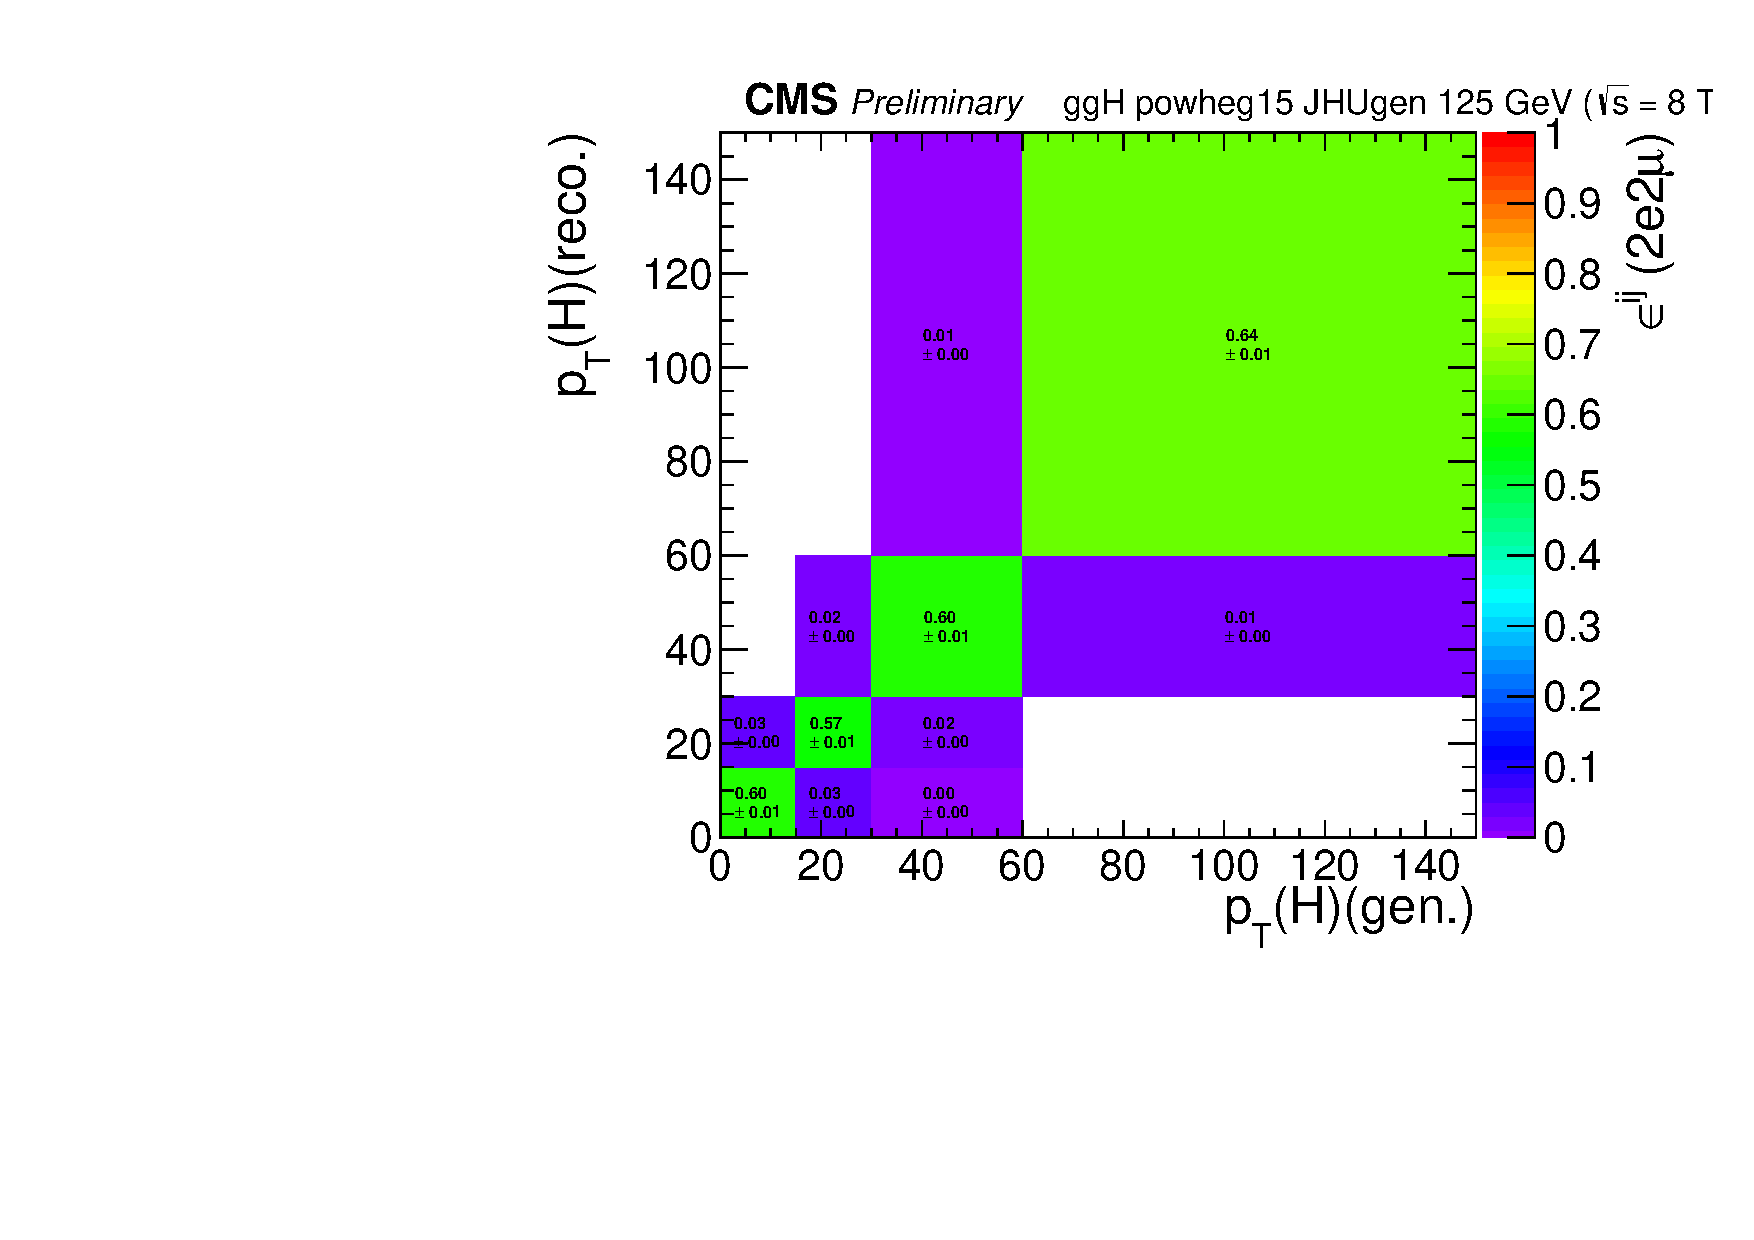
\includegraphics[width=0.48\textwidth,angle=0]{Plots/eff2d_ggH_powheg15_JHUgen_125_pT4l_2e2mu.pdf}
    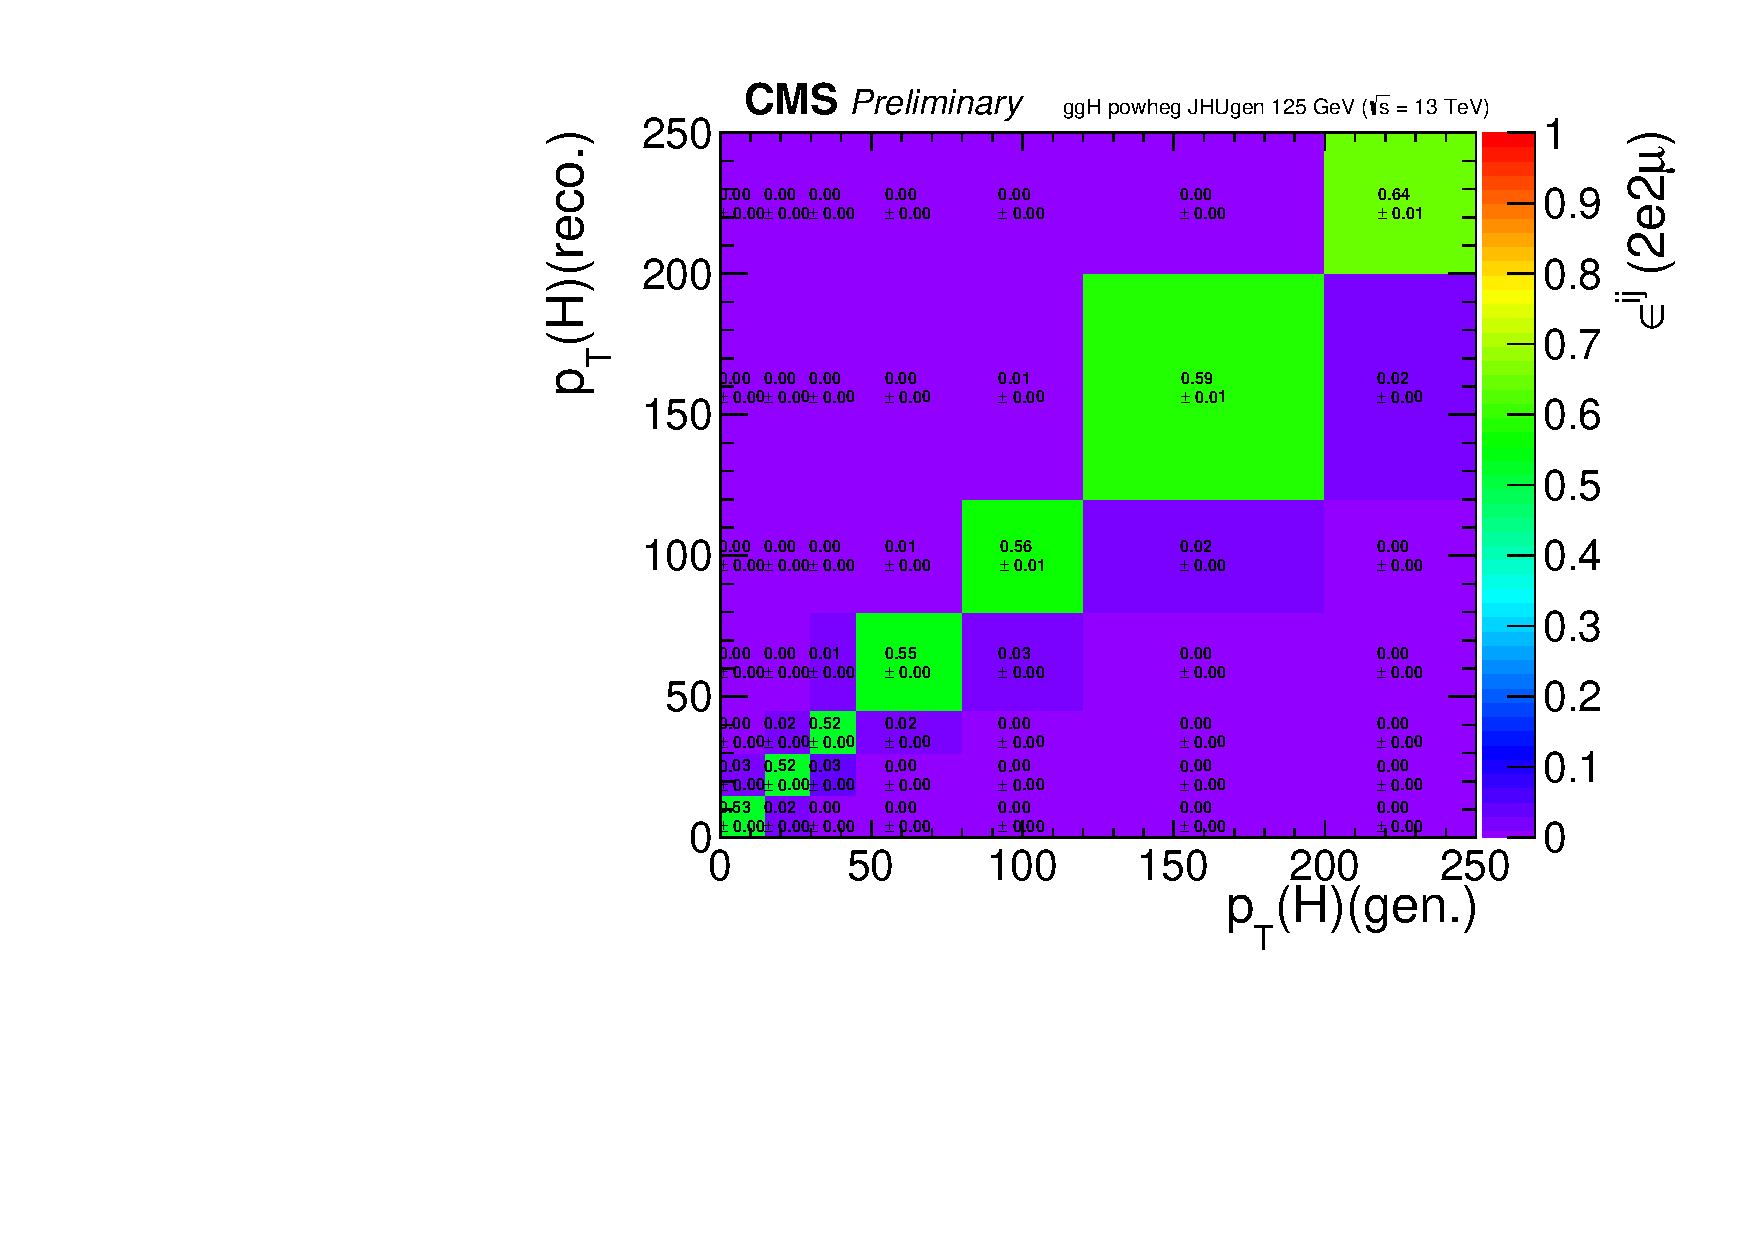
\includegraphics[width=0.48\textwidth,angle=0]{Plots/eff2d_ggH_powheg_JHUgen_125_pT4l_2e2mu.pdf}
    \label{fig:eff-pT4l-2e2mu-maintext:a}
    }
    \subfigure[$gg\rightarrow$H ({\sc minloHJJ})]{
    %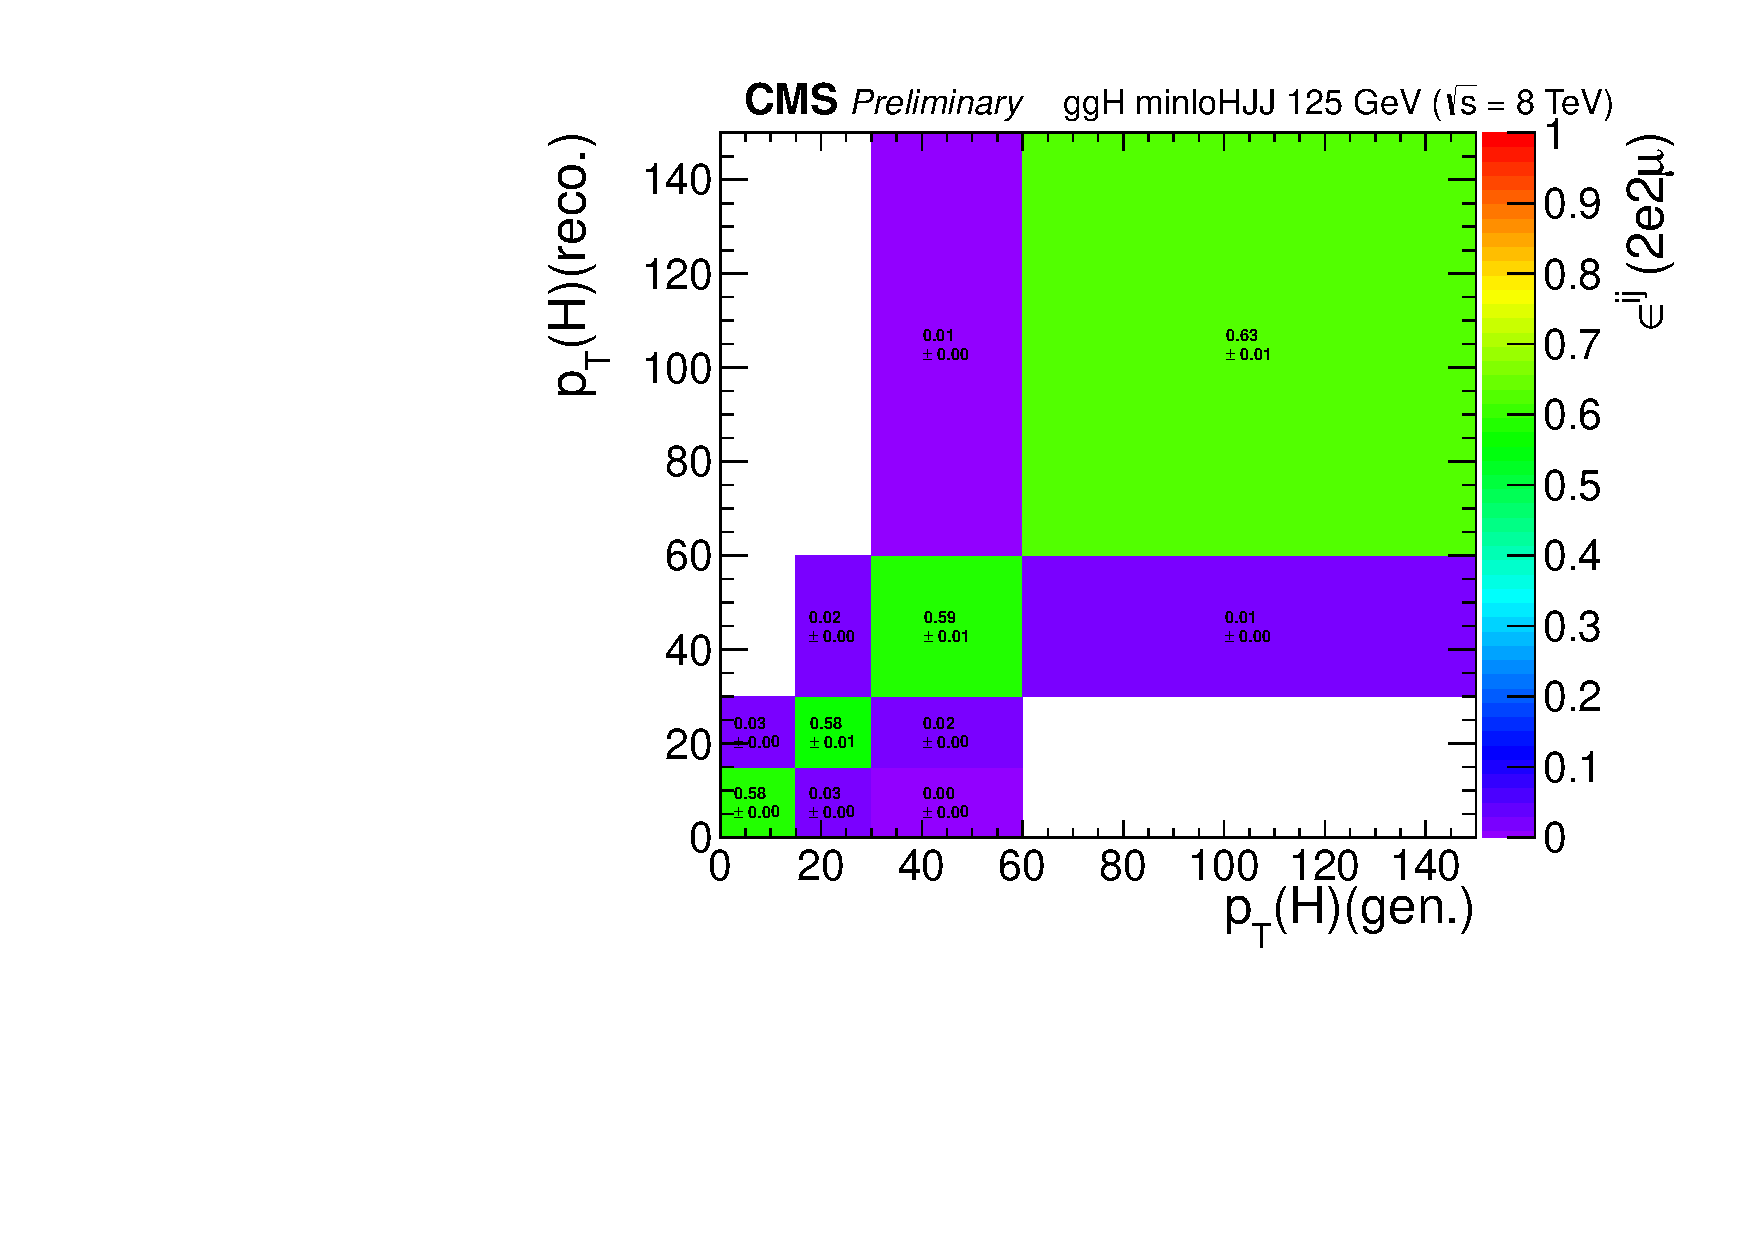
\includegraphics[width=0.48\textwidth,angle=0]{Plots/eff2d_ggH_minloHJJ_125_pT4l_2e2mu.pdf}
    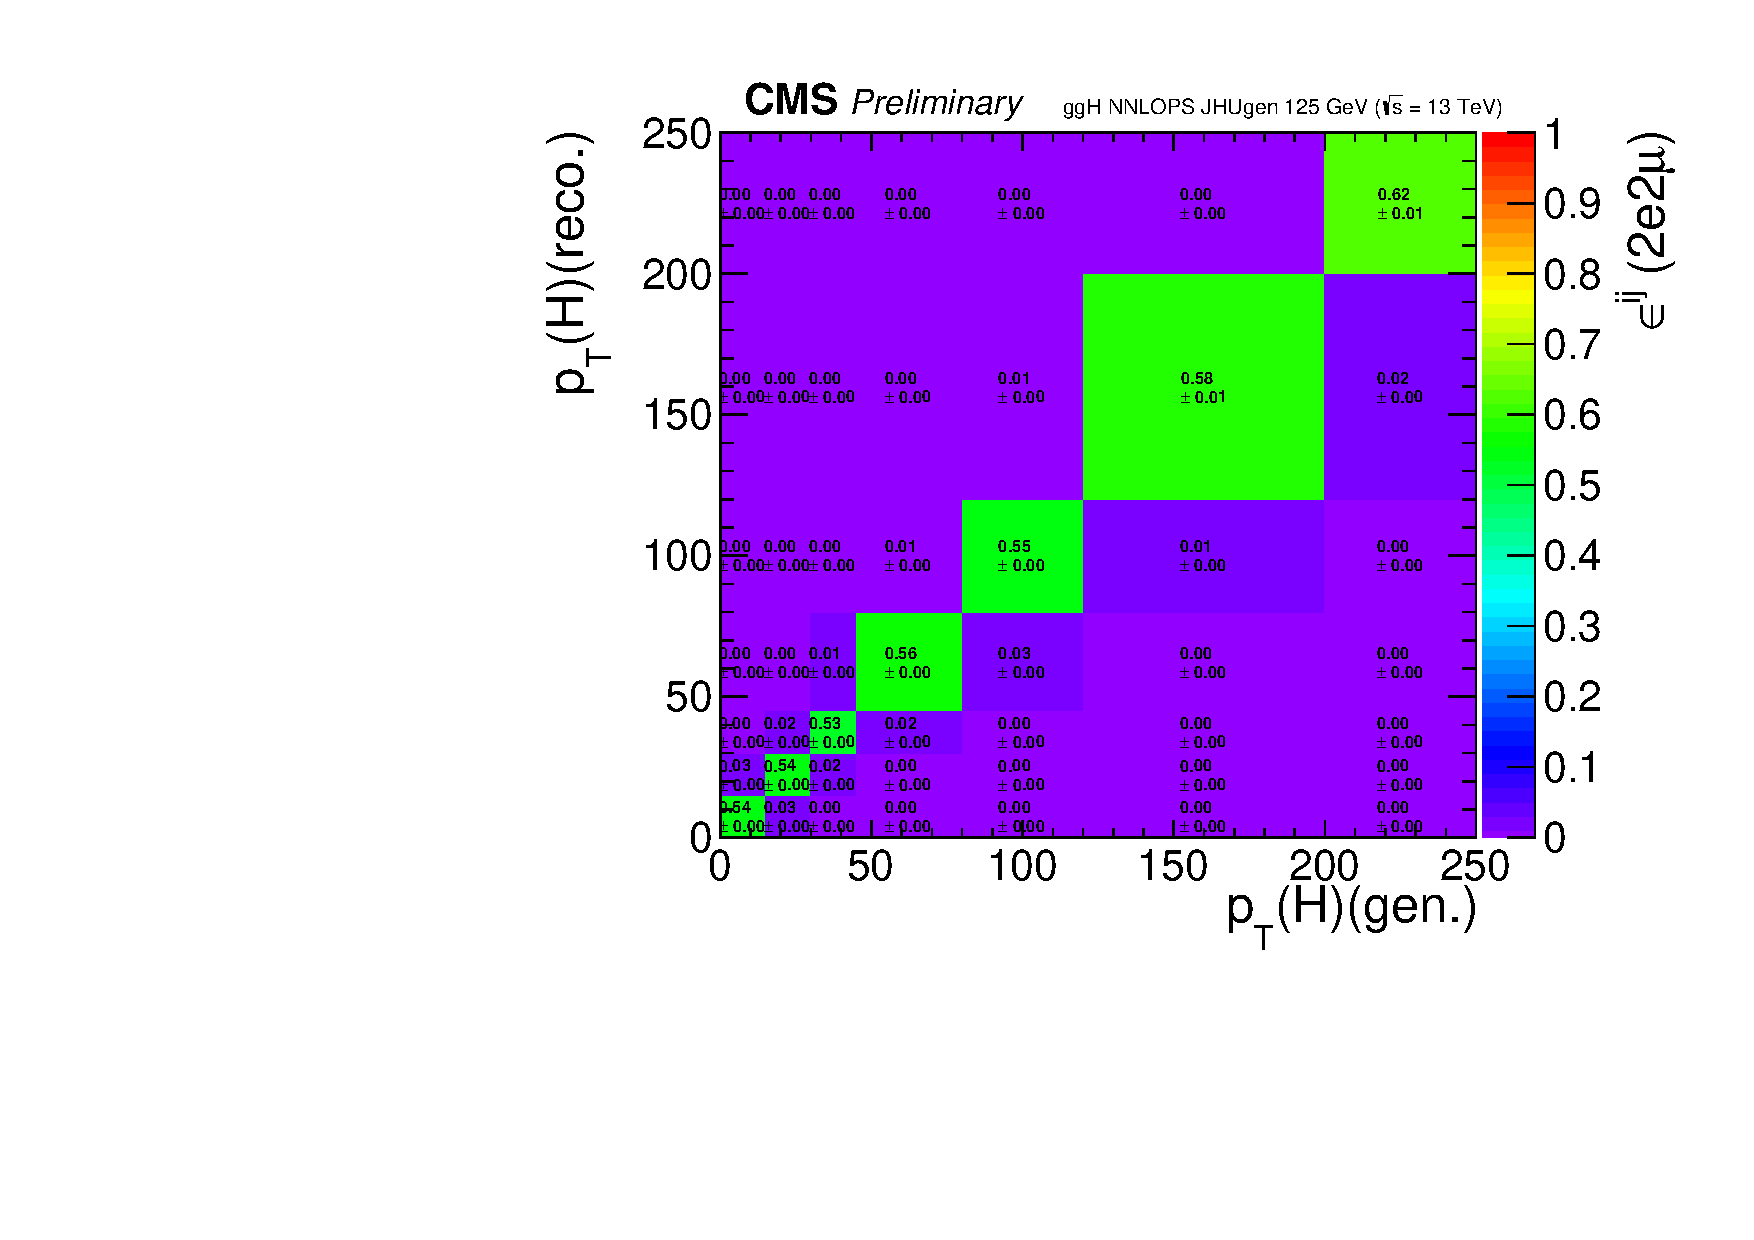
\includegraphics[width=0.48\textwidth,angle=0]{Plots/eff2d_ggH_NNLOPS_JHUgen_125_pT4l_2e2mu.pdf}
    \label{fig:eff-pT4l-2e2mu-maintext:b}
    } \\
    \subfigure[VBF ({\sc powheg})]{
    %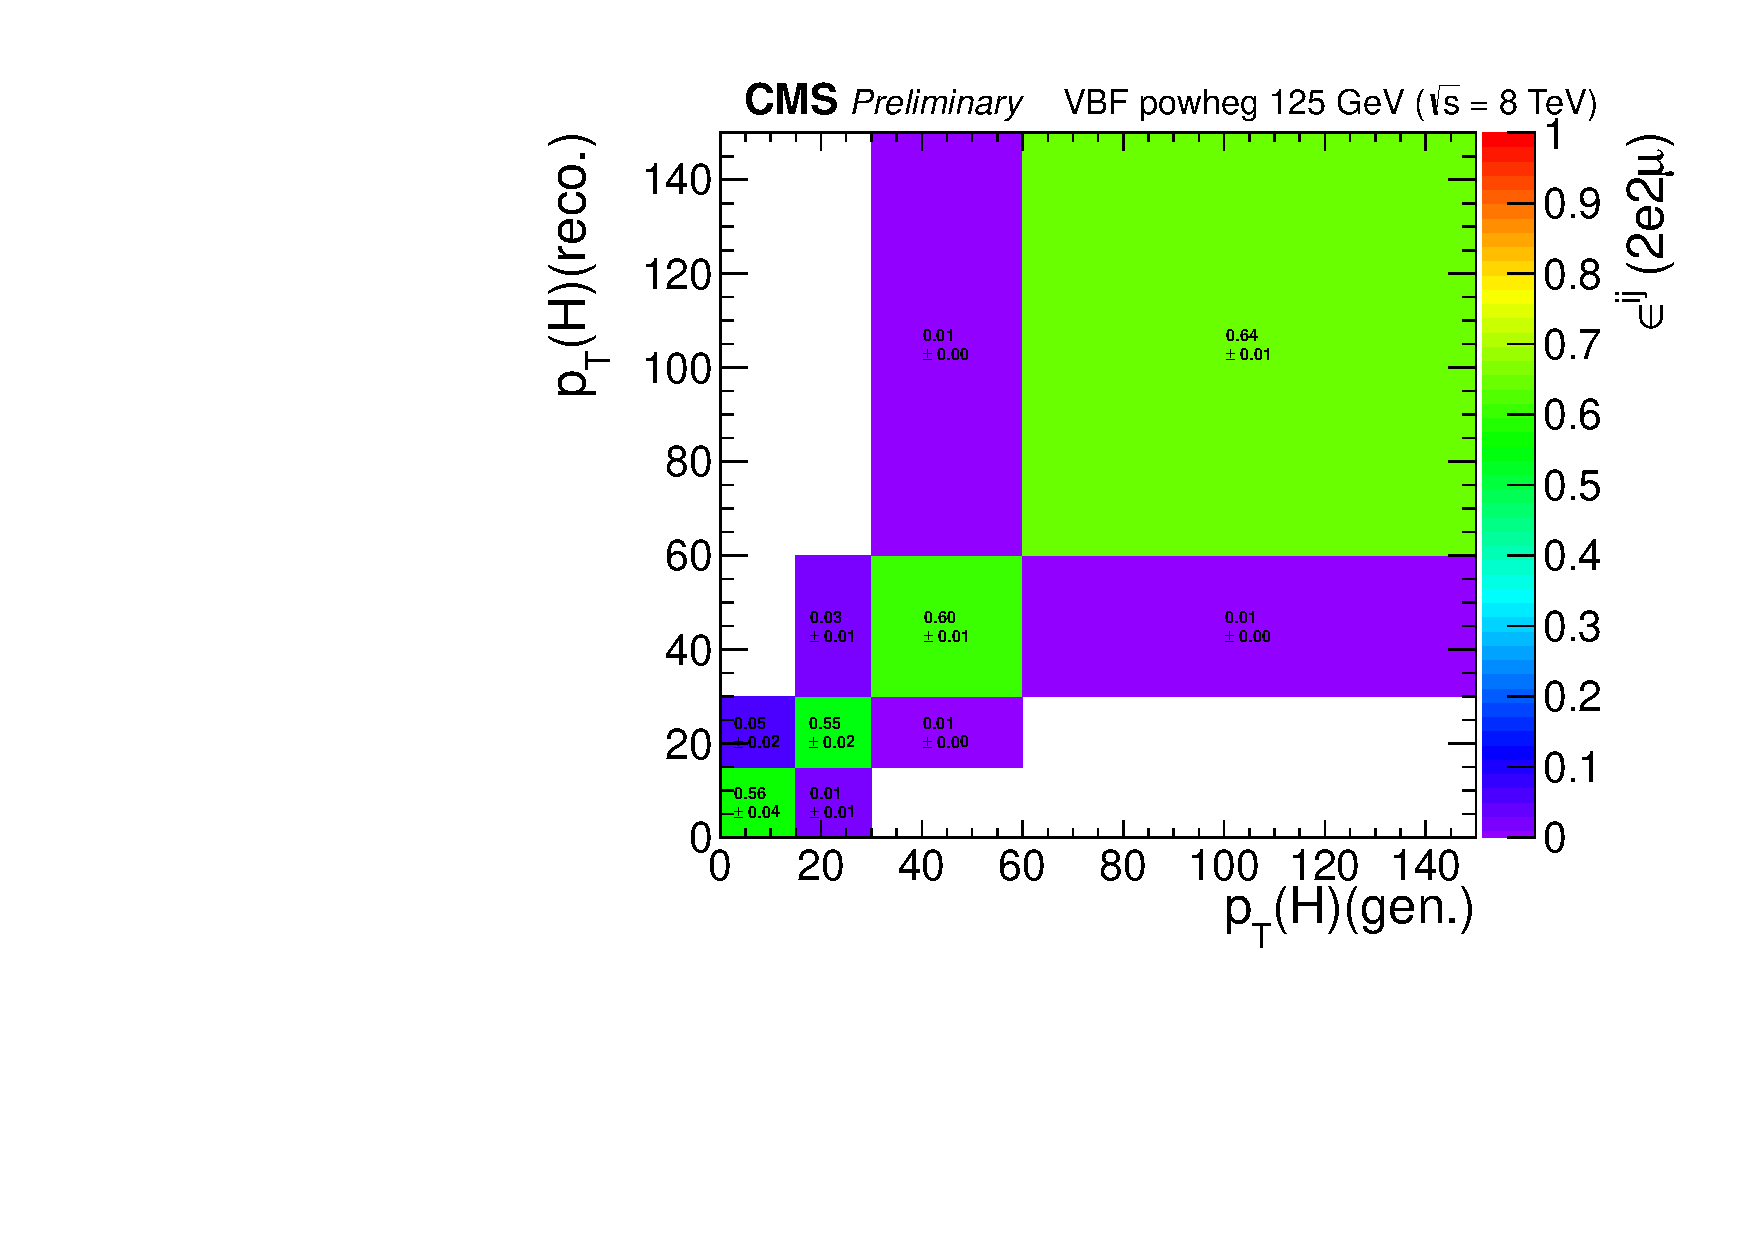
\includegraphics[width=0.48\textwidth,angle=0]{Plots/eff2d_VBF_powheg_125_pT4l_2e2mu.pdf}
    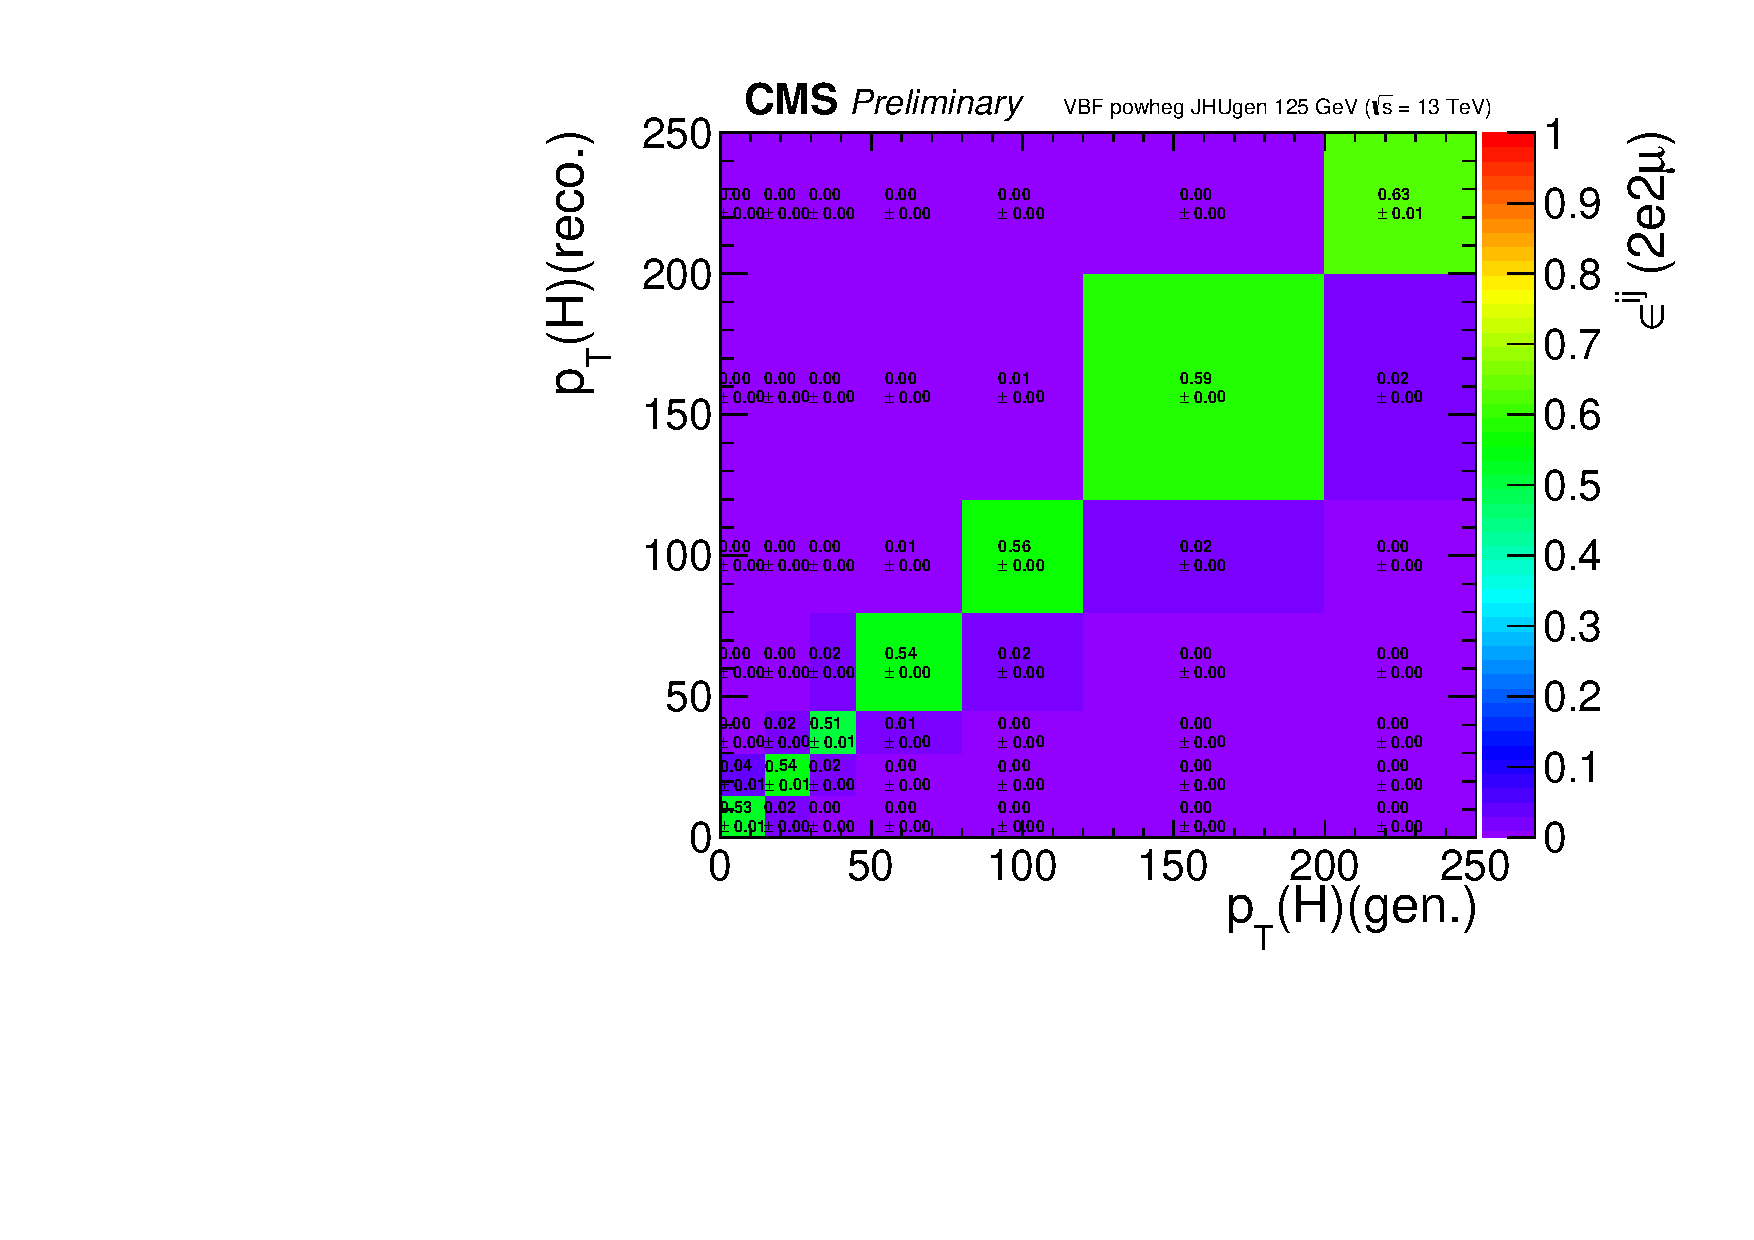
\includegraphics[width=0.48\textwidth,angle=0]{Plots/eff2d_VBF_powheg_JHUgen_125_pT4l_2e2mu.pdf}
    \label{fig:eff-pT4l-2e2mu-maintext:c}
    }
    \subfigure[WH ({\sc pythia})]{
    %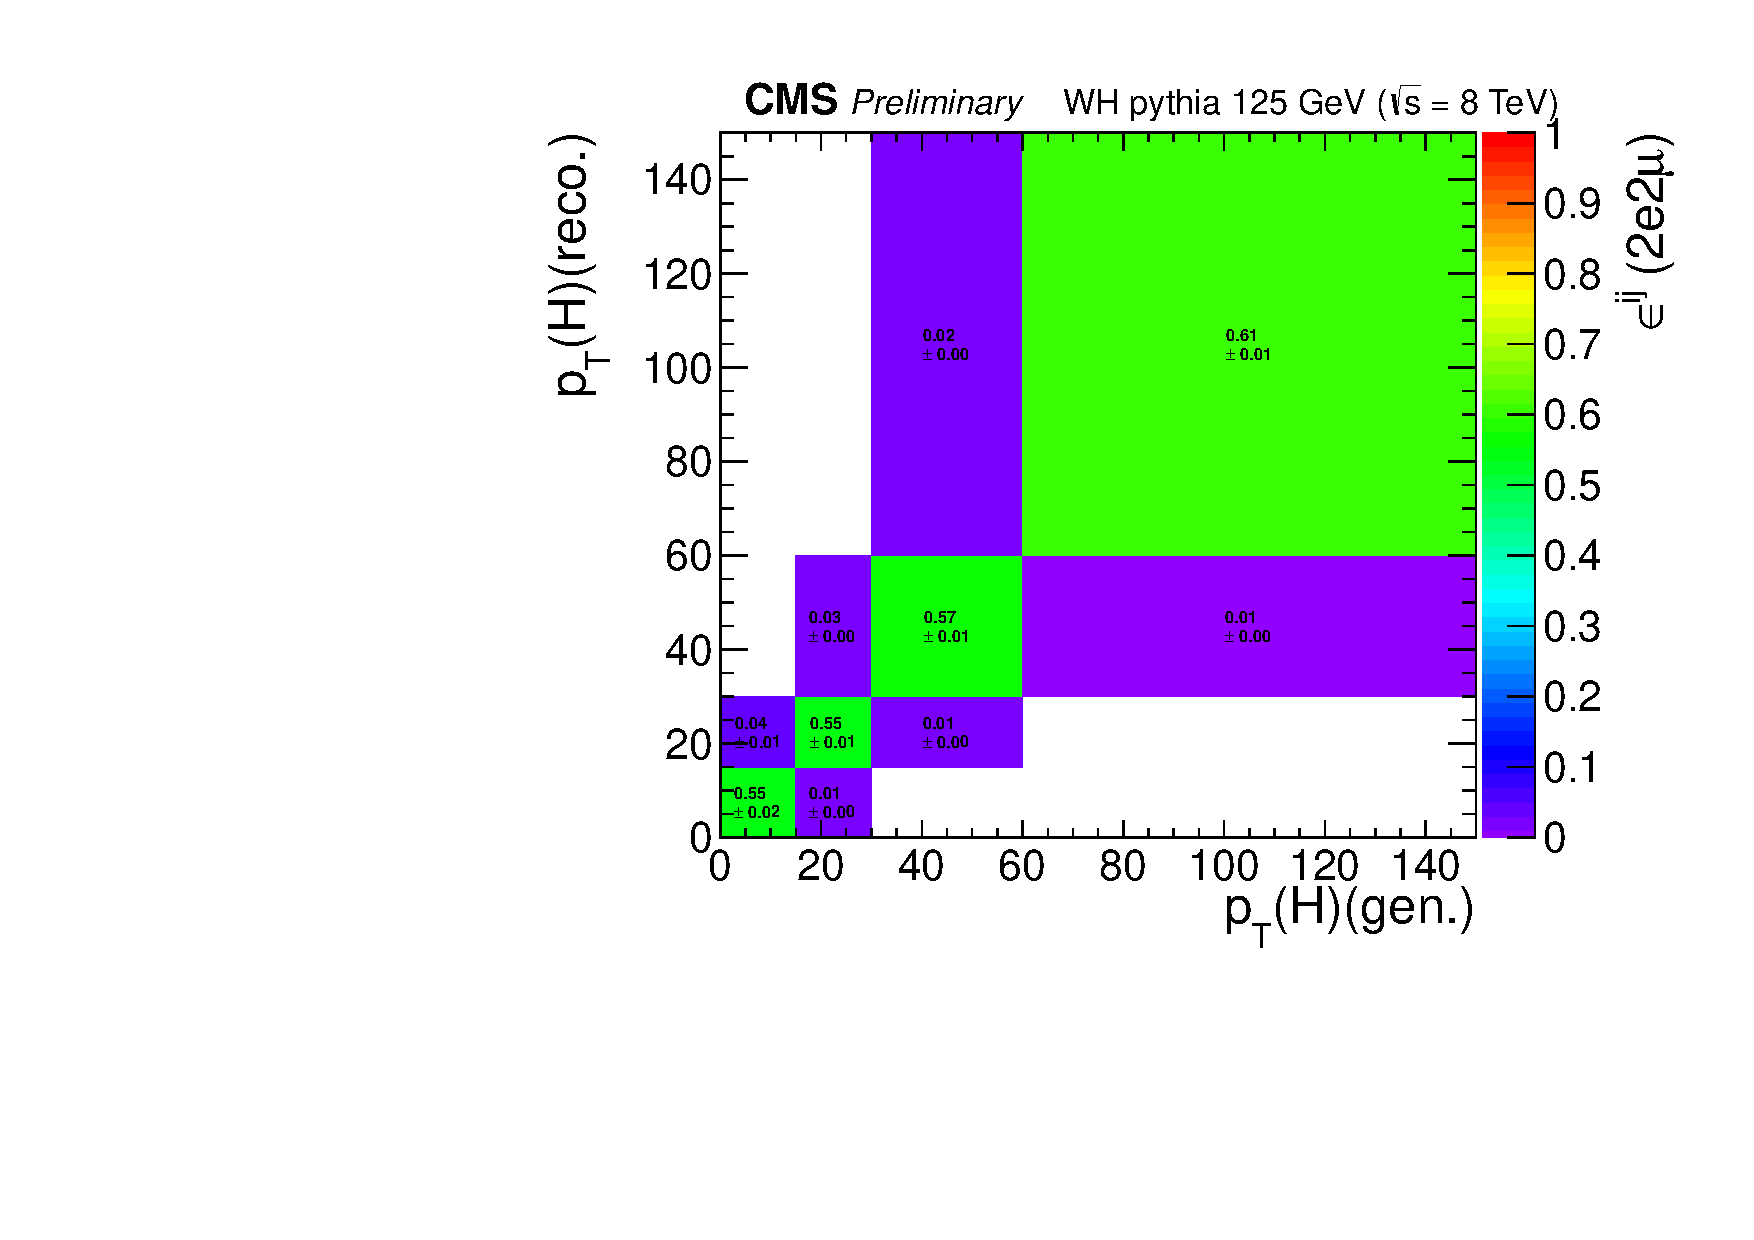
\includegraphics[width=0.48\textwidth,angle=0]{Plots/eff2d_WH_pythia_125_pT4l_2e2mu.pdf}
    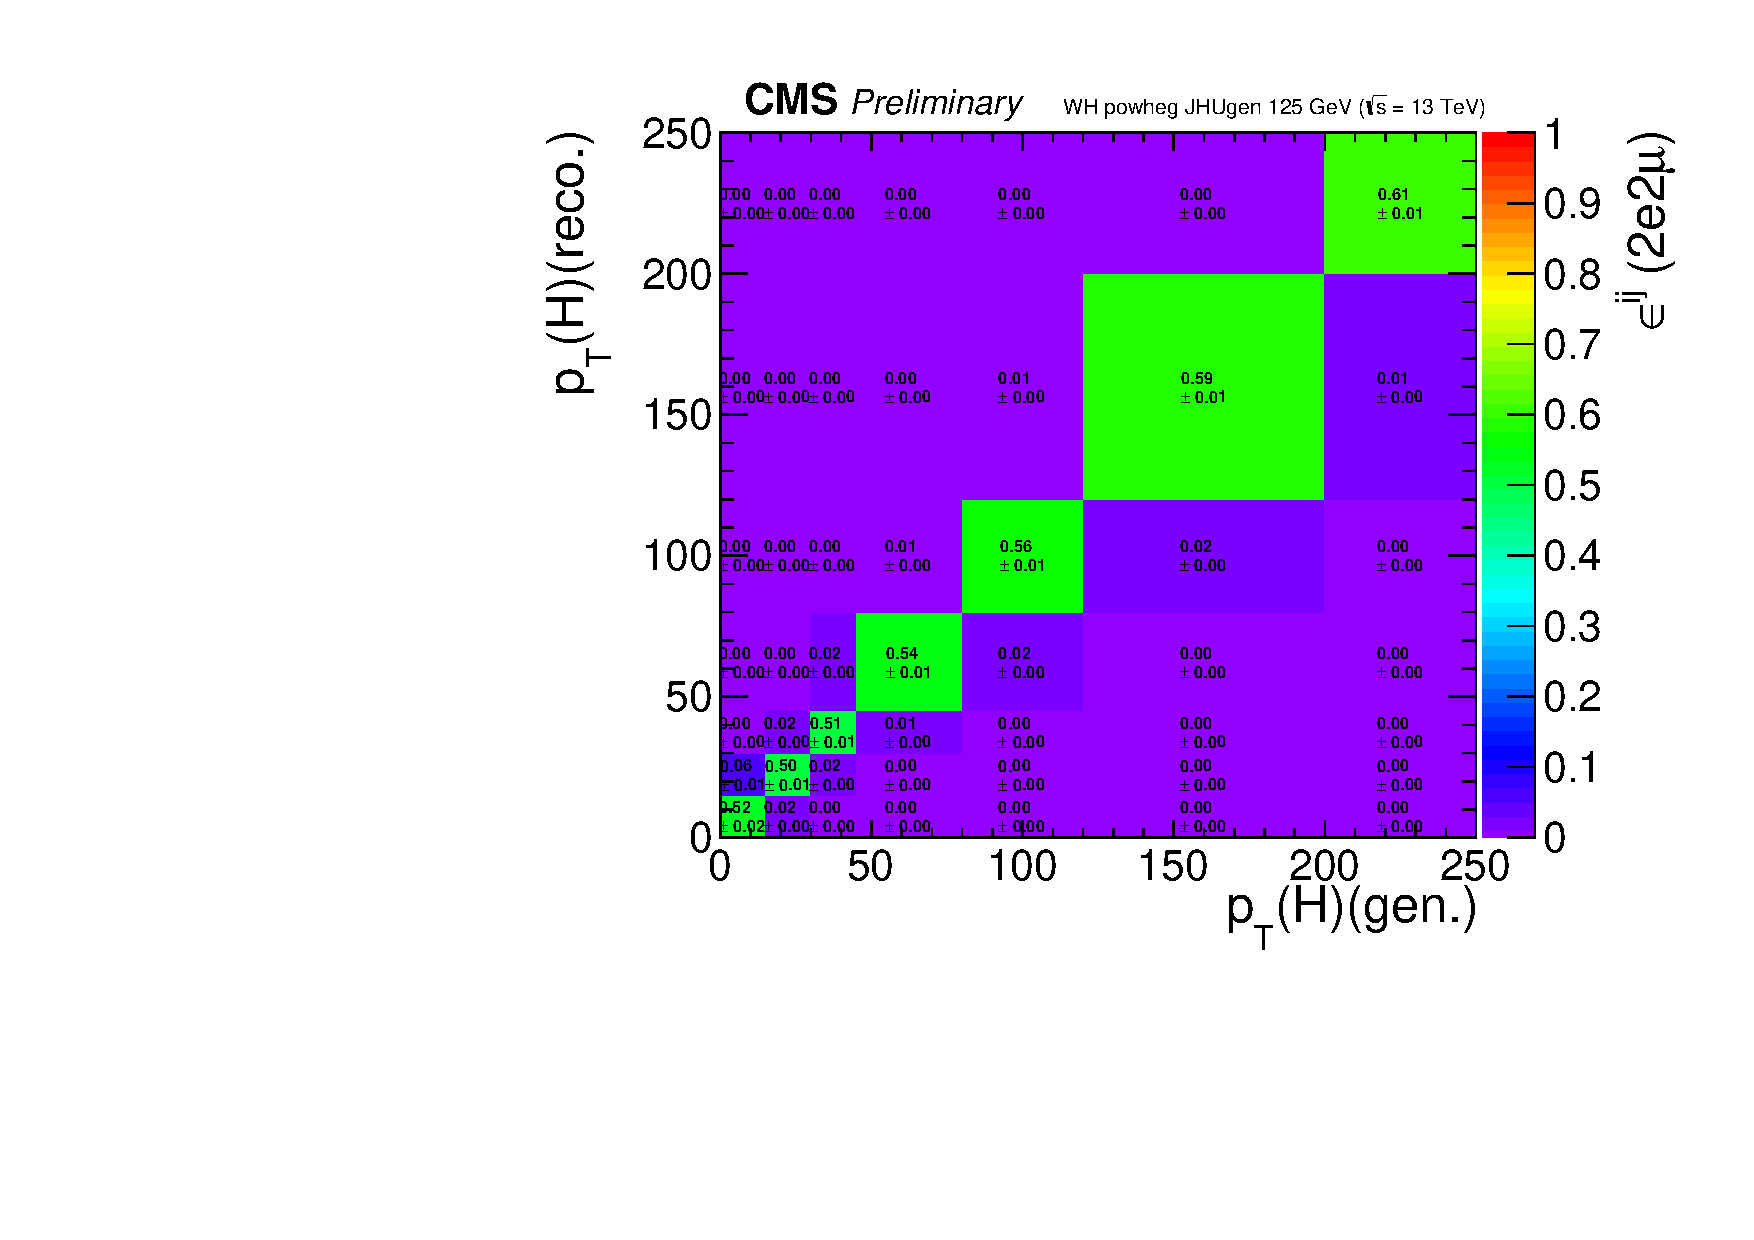
\includegraphics[width=0.48\textwidth,angle=0]{Plots/eff2d_WH_powheg_JHUgen_125_pT4l_2e2mu.pdf}
    \label{fig:eff-pT4l-2e2mu-maintext:d}
    } \\
    \subfigure[ZH ({\sc pythia})]{
    %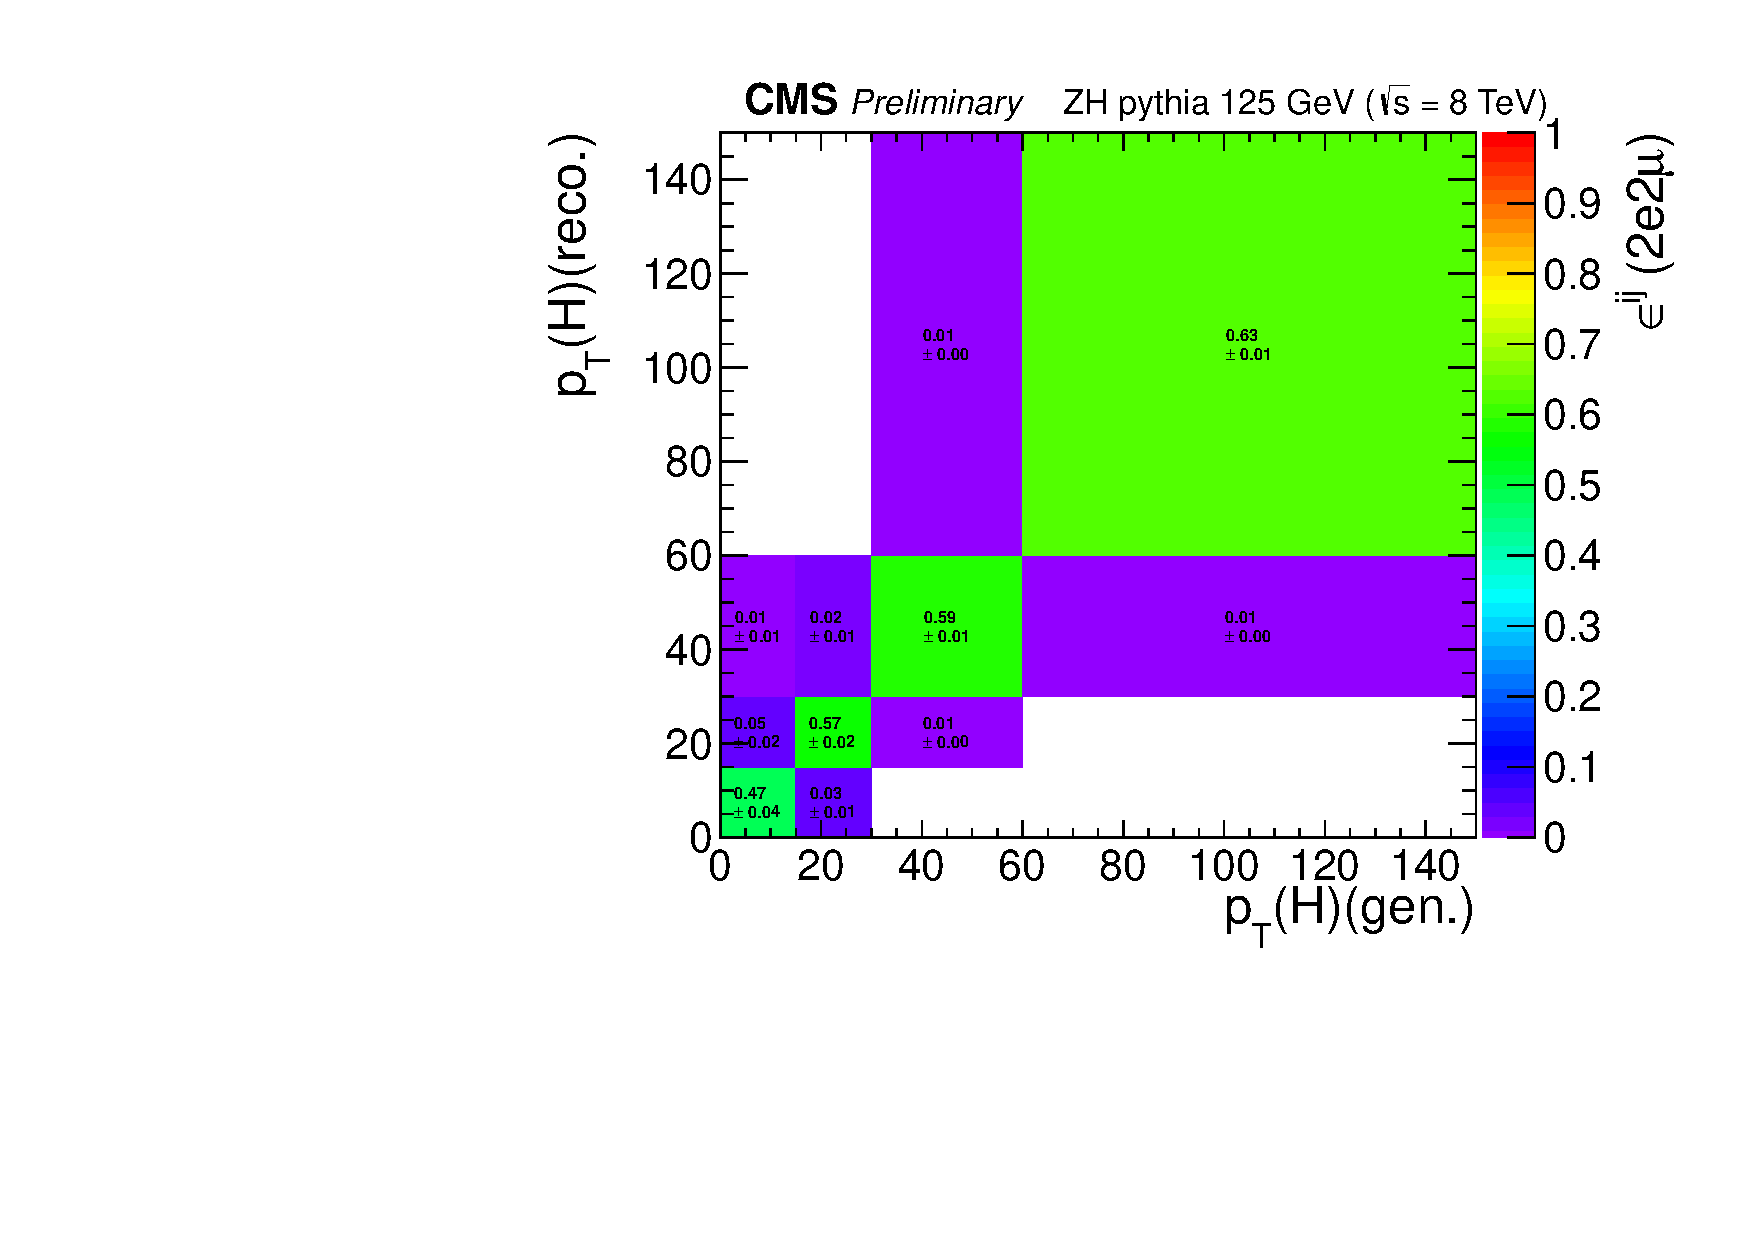
\includegraphics[width=0.48\textwidth,angle=0]{Plots/eff2d_ZH_pythia_125_pT4l_2e2mu.pdf}
    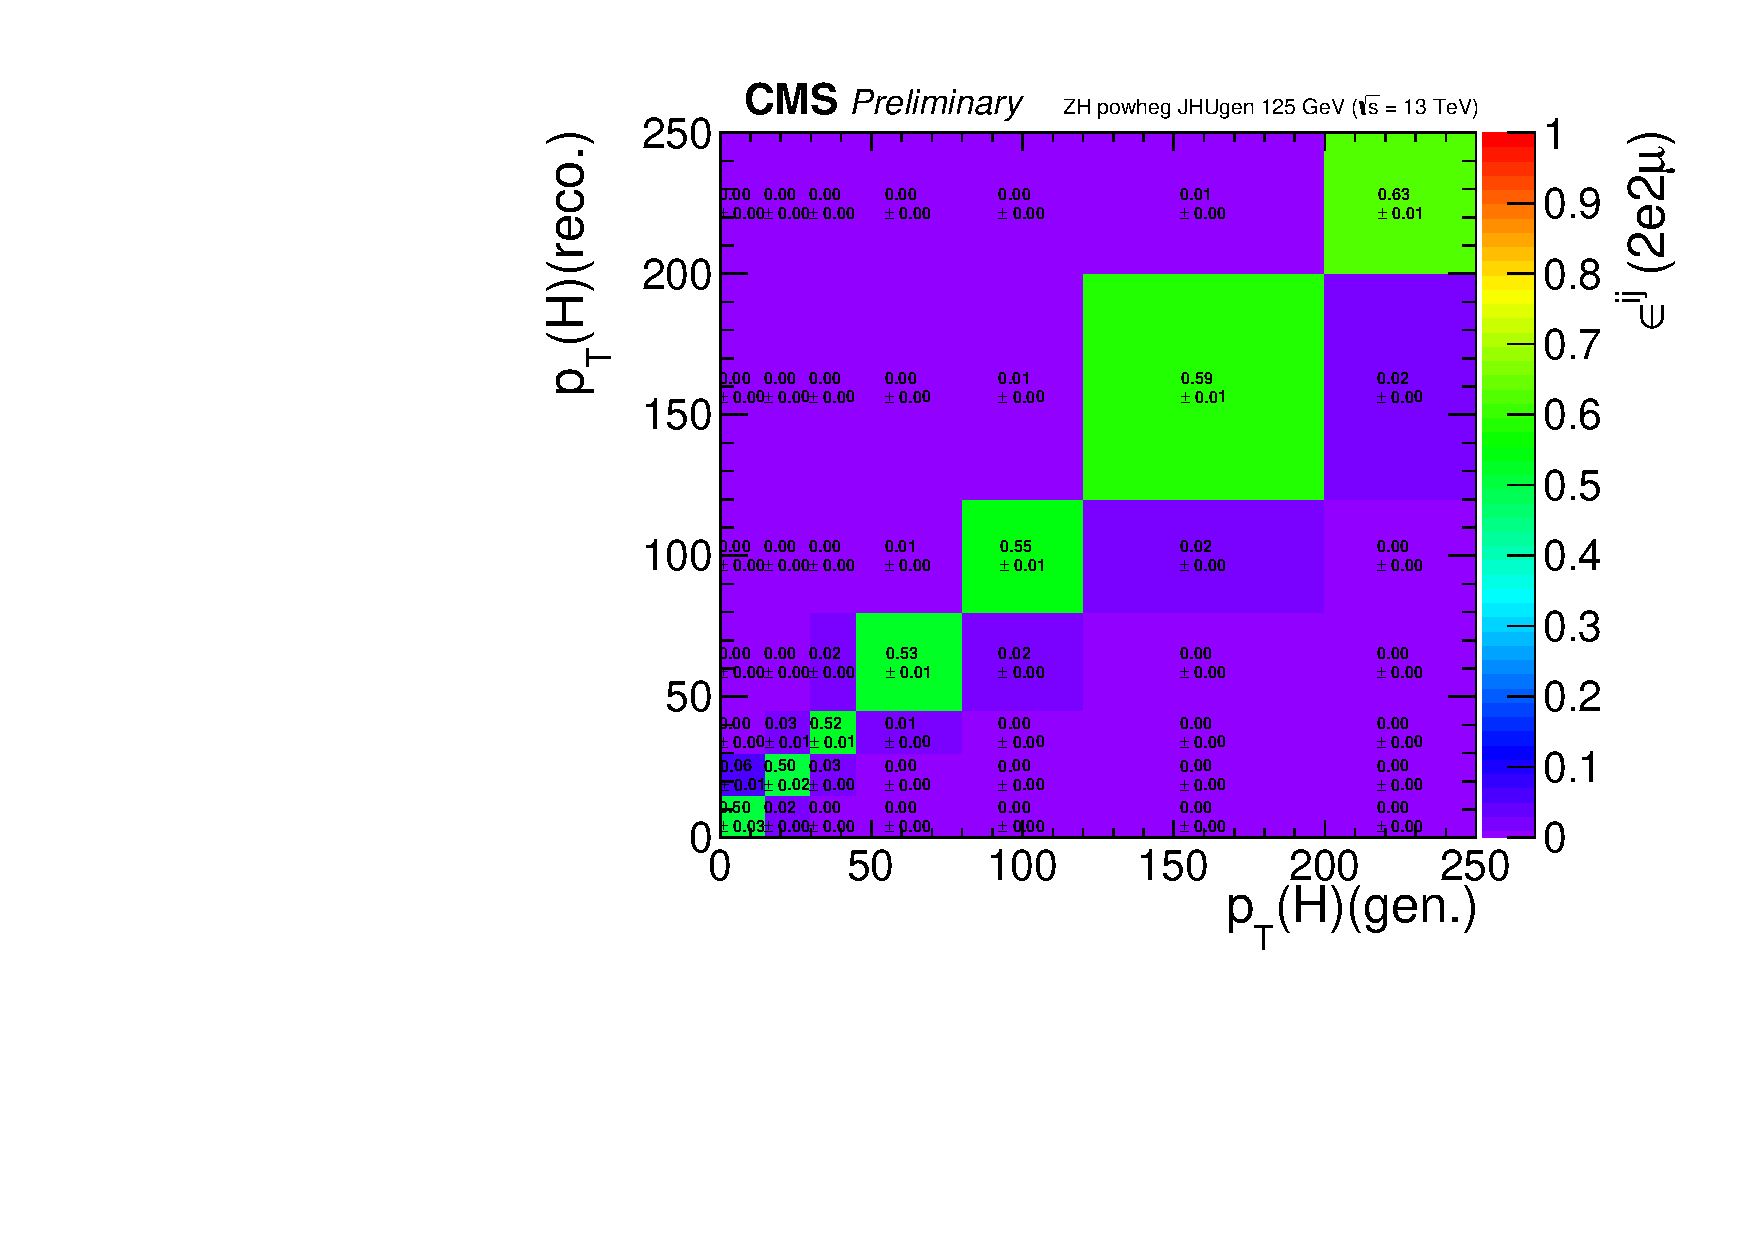
\includegraphics[width=0.48\textwidth,angle=0]{Plots/eff2d_ZH_powheg_JHUgen_125_pT4l_2e2mu.pdf}
    \label{fig:eff-pT4l-2e2mu-maintext:e}
    }
    \subfigure[ttH ({\sc pythia})]{
    %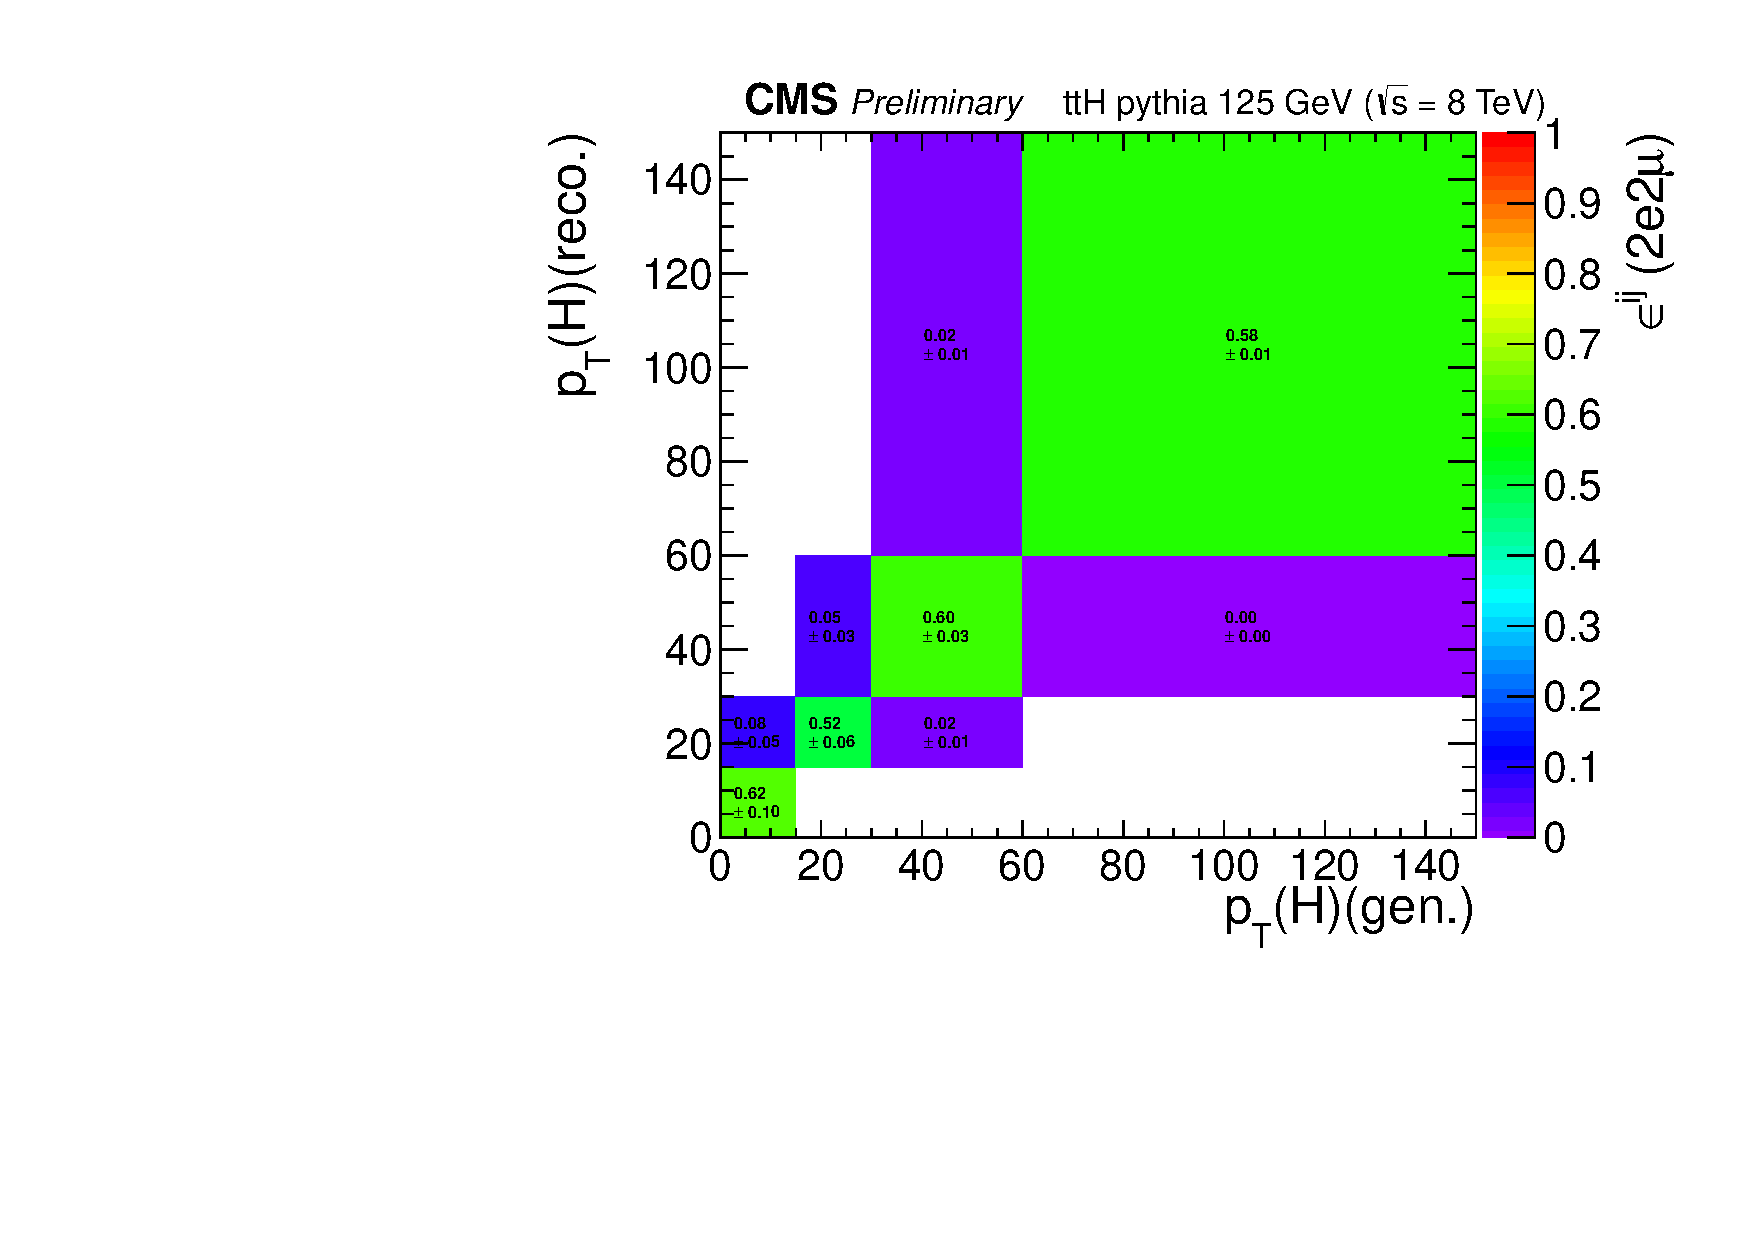
\includegraphics[width=0.48\textwidth,angle=0]{Plots/eff2d_ttH_pythia_125_pT4l_2e2mu.pdf}
    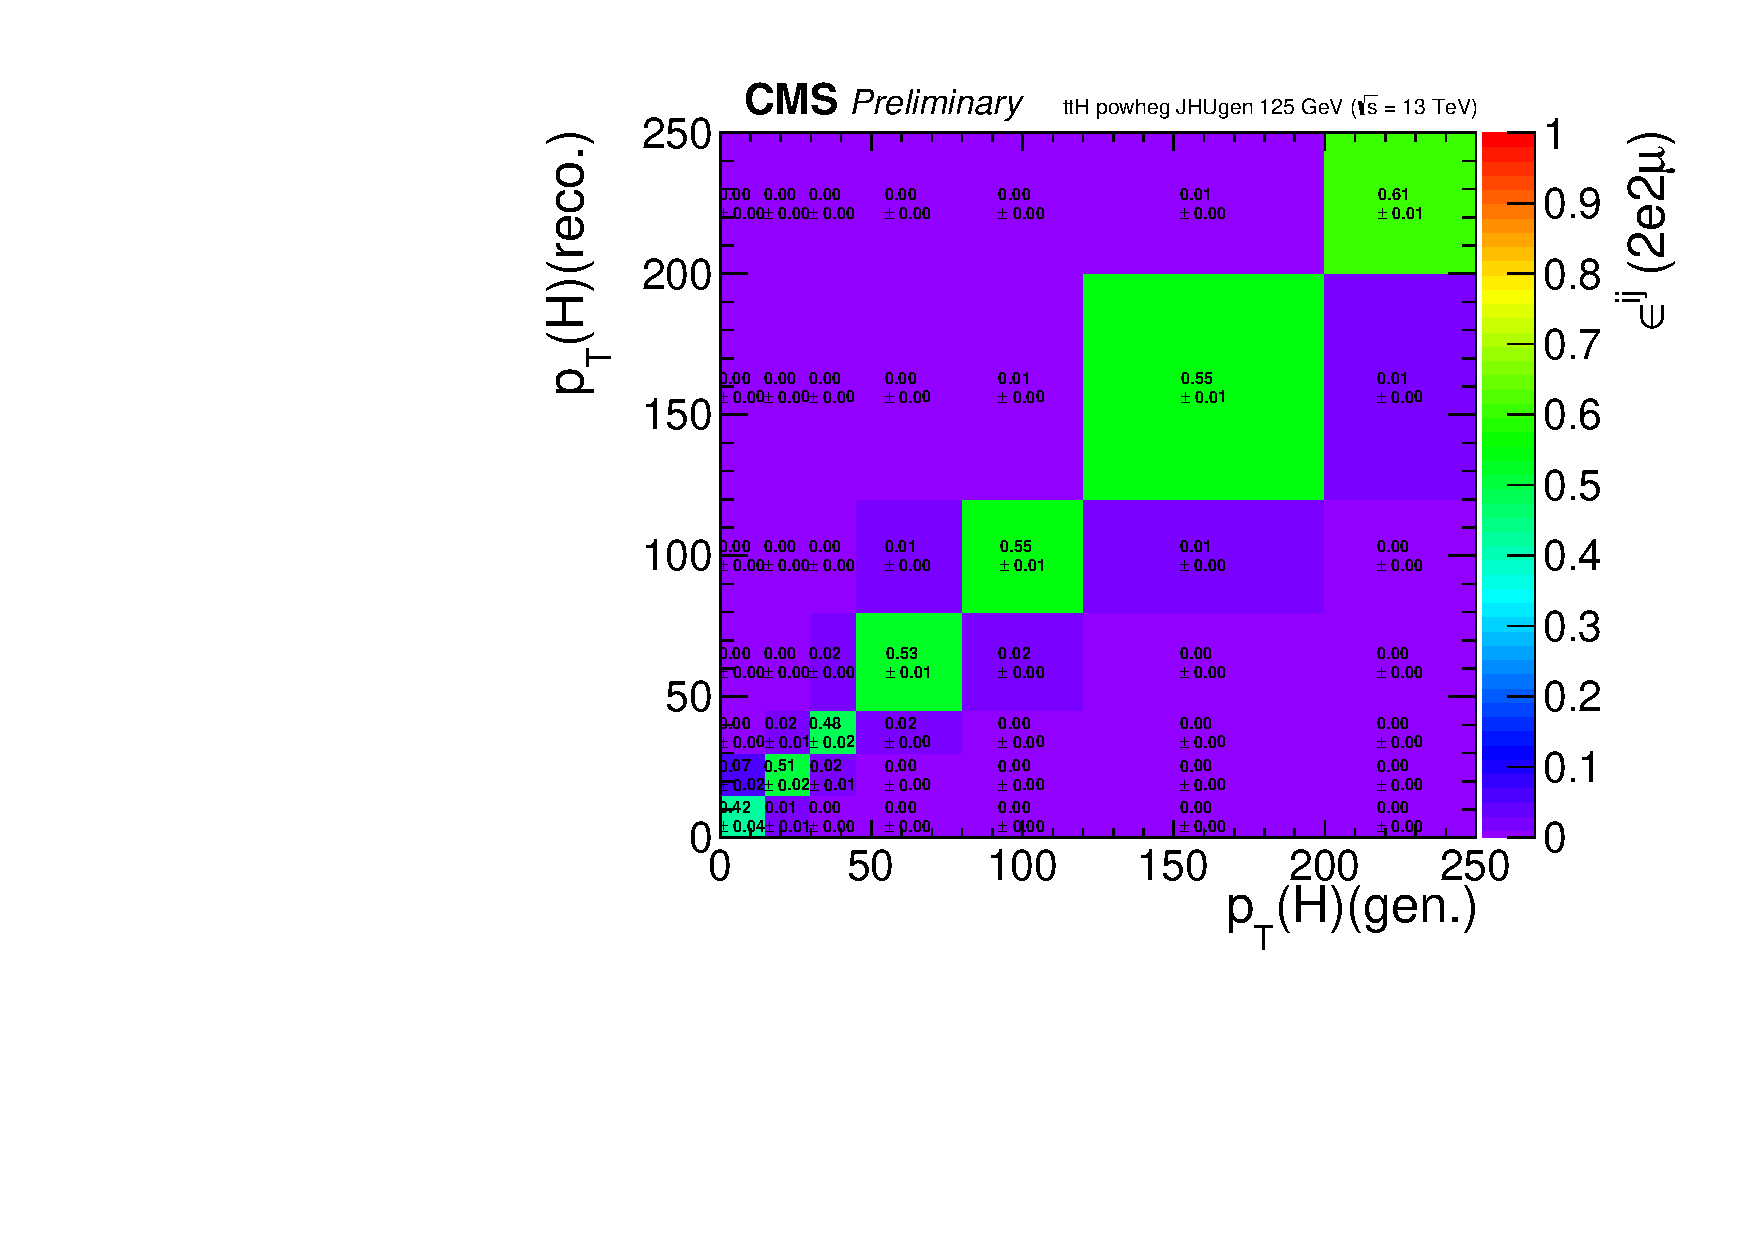
\includegraphics[width=0.48\textwidth,angle=0]{Plots/eff2d_ttH_powheg_JHUgen_125_pT4l_2e2mu.pdf}
    \label{fig:eff-pT4l-2e2mu-maintext:f}
    }
    \caption{ Efficiency matrices for $\pt({\rm H})$ for different SM production modes in the $2e2\mu$ final state using 2018 samples. }
    \label{fig:eff-pT4l-2e2mu-maintext}
  \end{center}
\end{figure} \clearpage
%%%%%%%
Figure~\ref{fig:sigfits-asimov-SM-pt4l-4l} shows the four lepton mass distributions for an Asimov dataset generated using SM cross section values and efficiencies 
from the gg$\rightarrow$H production mode from {\sc powheg+JHUgen}, and resulting fitted values of the signal and background pdfs in different bins
of $\pt(\mathrm{H})$ (all final states combined).
%The same distributions and resulting fitted values of the signal and background pdfs in bins of all considered observables can be found in the Appendix~\ref{}.
% |0|15|30|45|80|120|200|13000|
\begin{figure}[htb]
  \begin{center}
    \subfigure[$0.0 \GeV < \pt(\mathrm{H}) < 15.0 \GeV$]{
      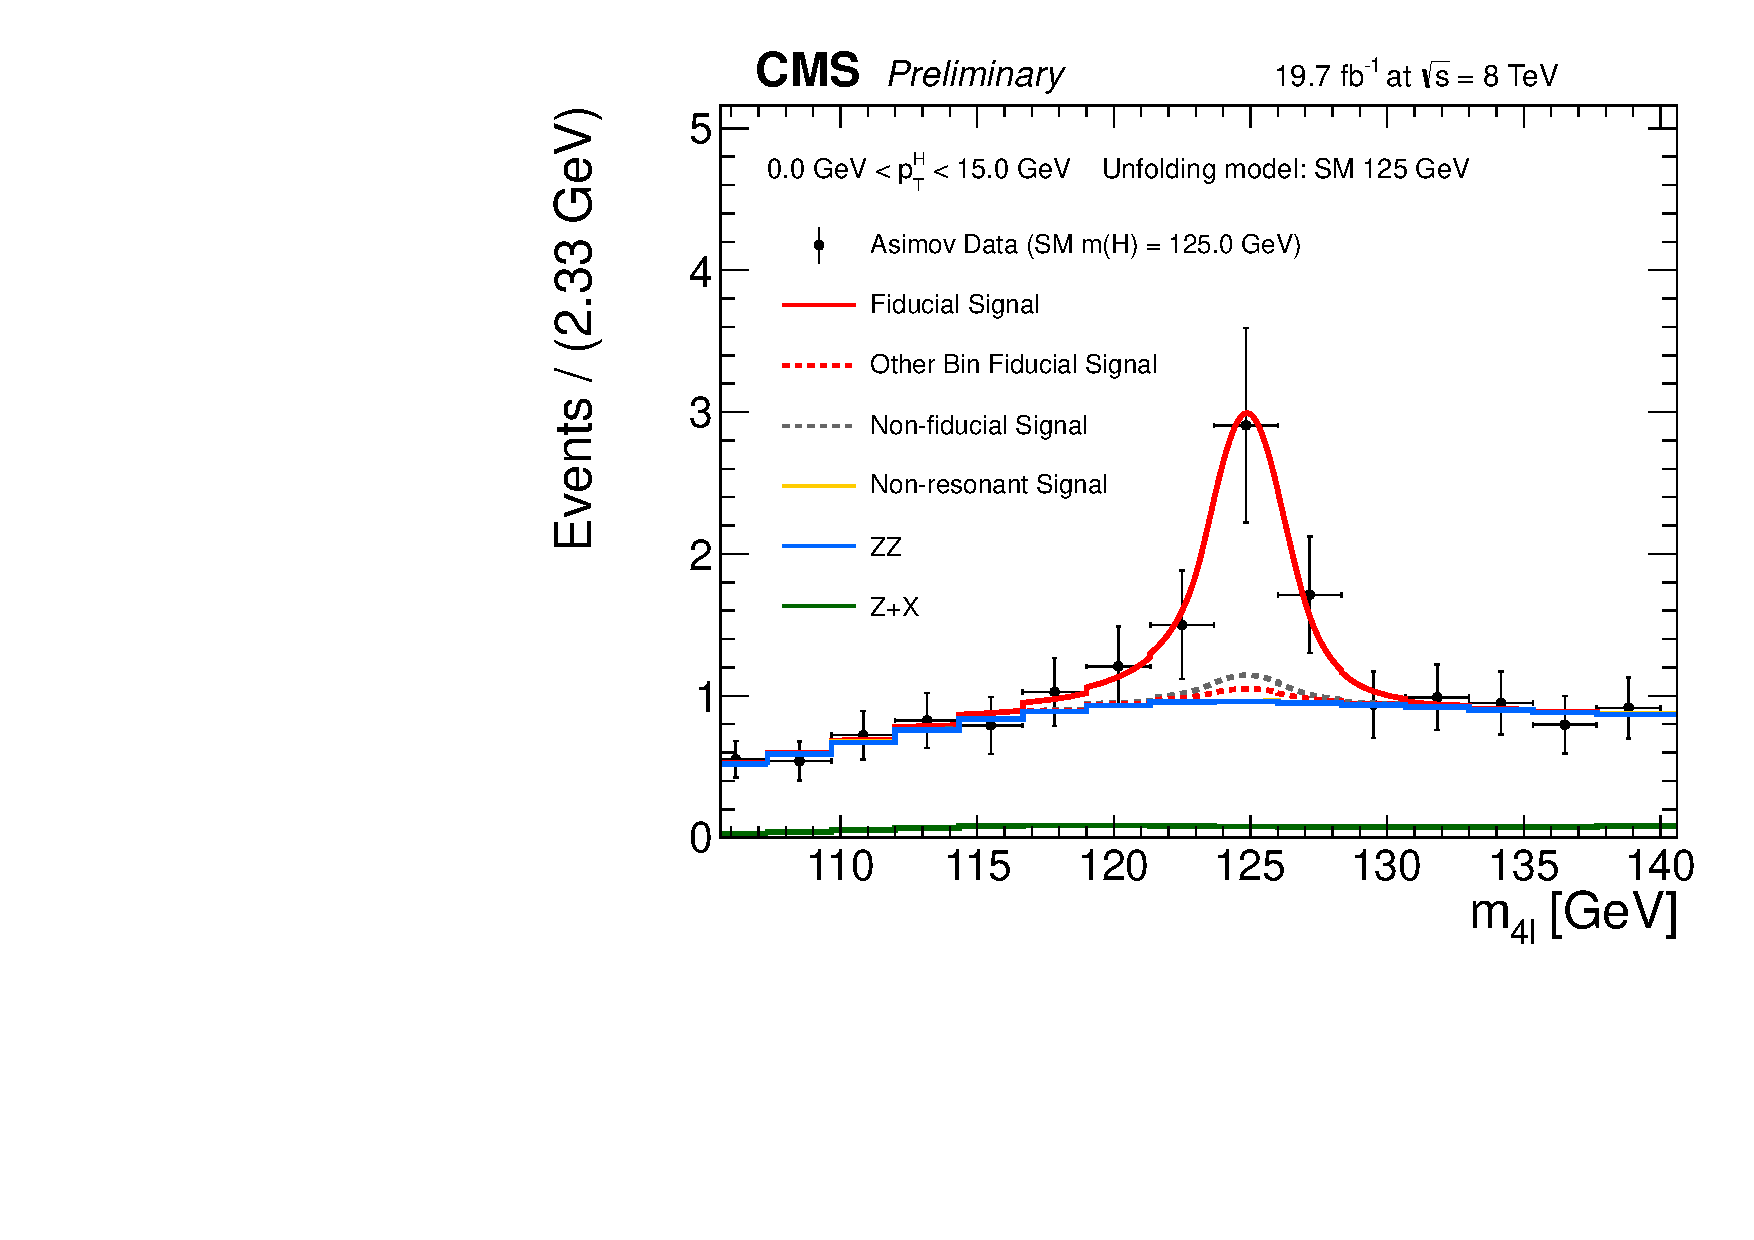
\includegraphics[width=0.40\textwidth,angle=0]{Plots/asimovdata_SM_125_v2_unfoldwith_SM_125_v3_pT4l_4l_recobin0.pdf}
       \label{fig:sigfits-asimov-SM-pT4l-4l:a}
    }
    \subfigure[$15.0 \GeV < \pt(\mathrm{H}) < 30.0 \GeV$]{
      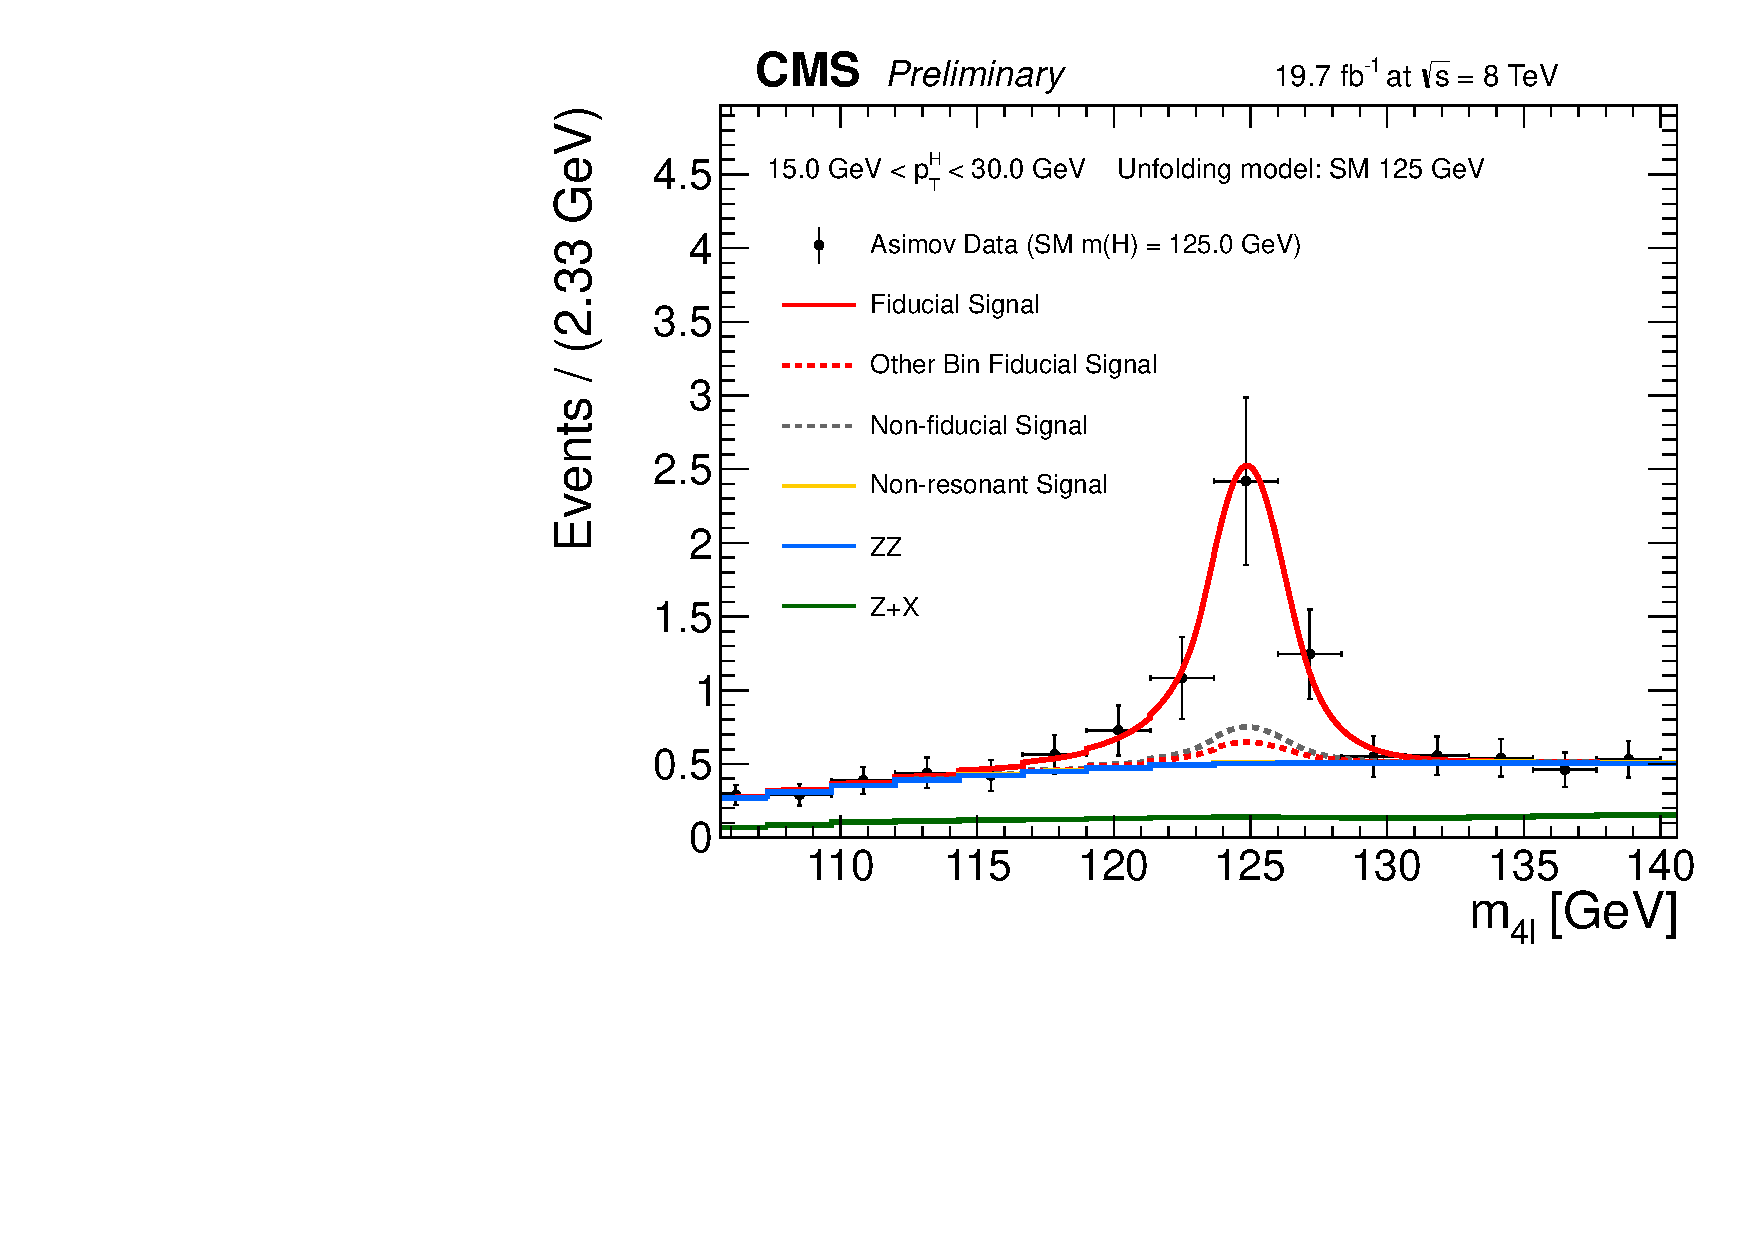
\includegraphics[width=0.40\textwidth,angle=0]{Plots/asimovdata_SM_125_v2_unfoldwith_SM_125_v3_pT4l_4l_recobin1.pdf}
       \label{fig:sigfits-asimov-SM-pT4l-4l:b}
    } \\
    \subfigure[$30.0 \GeV < \pt(\mathrm{H}) < 45.0 \GeV$]{
      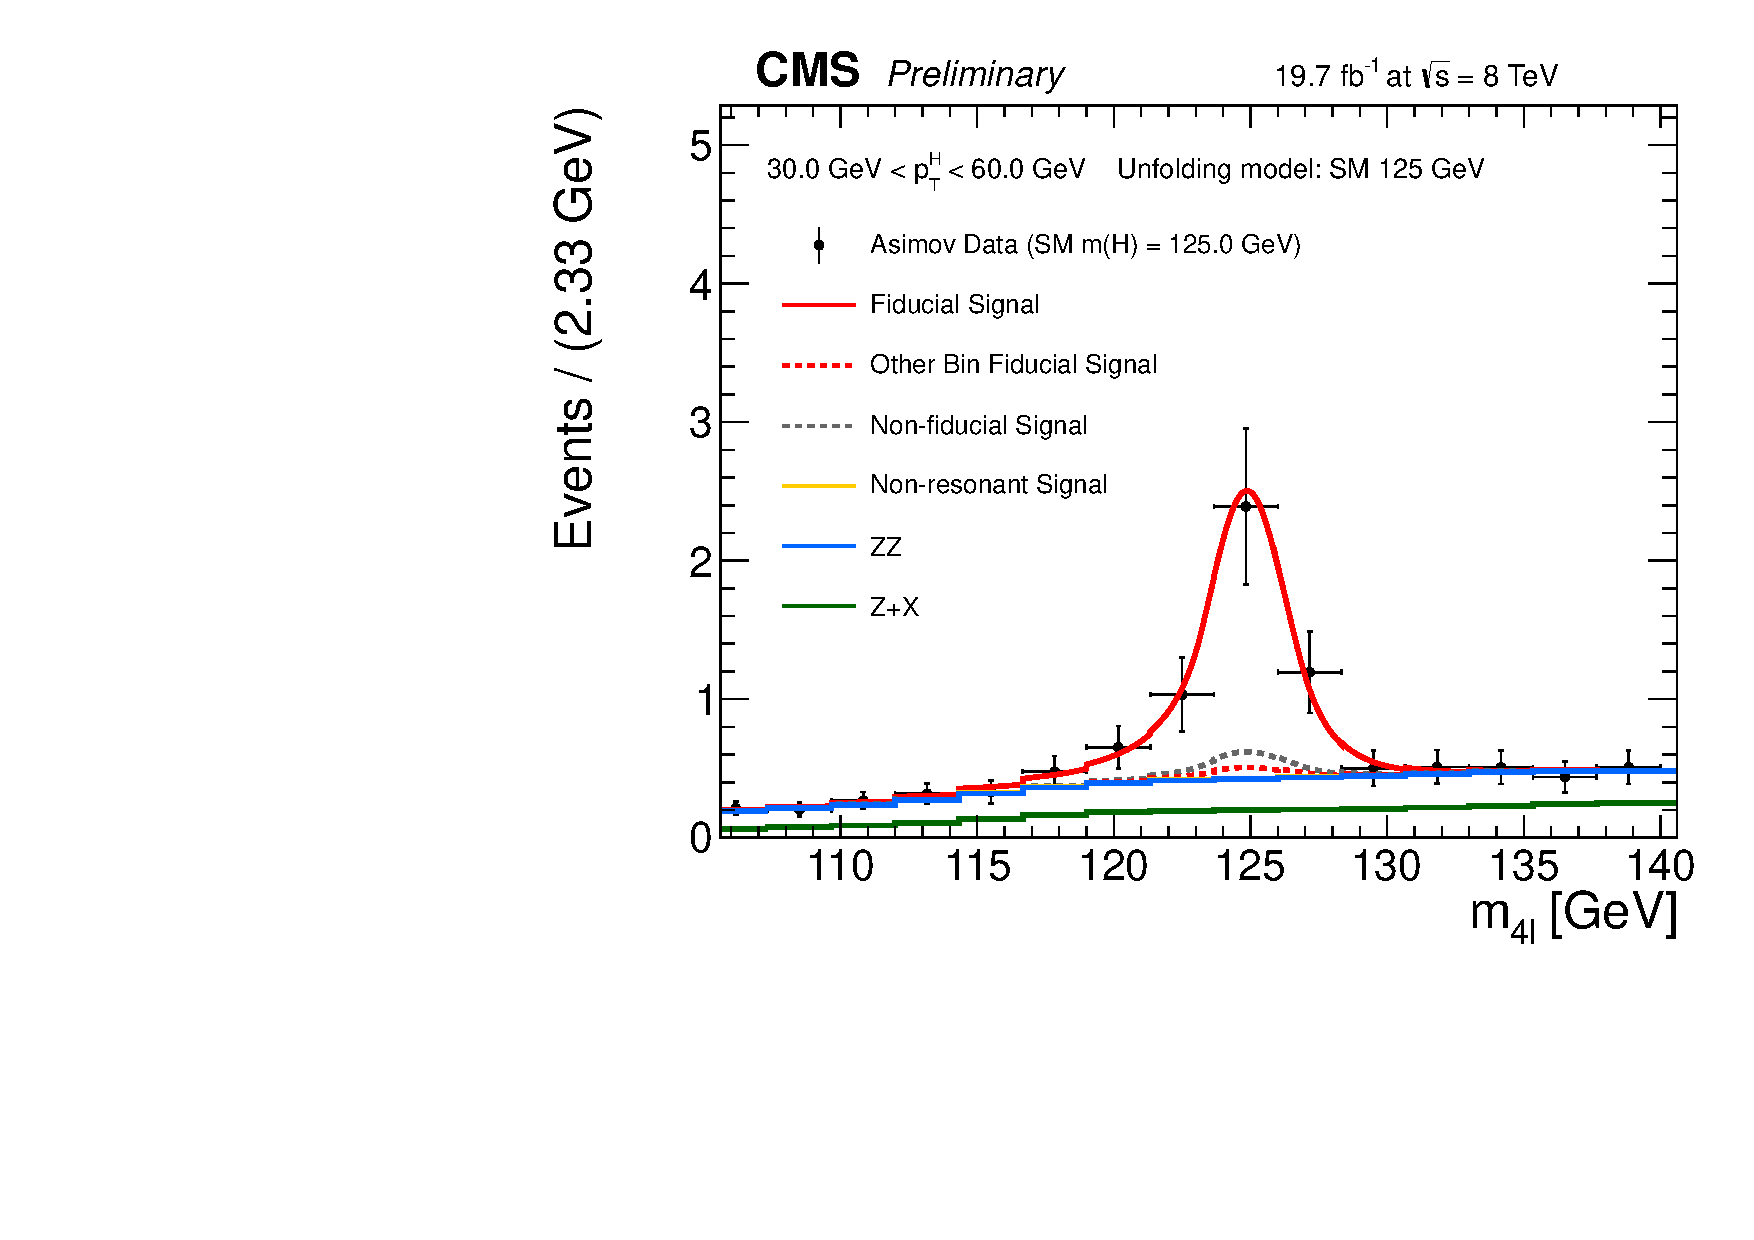
\includegraphics[width=0.40\textwidth,angle=0]{Plots/asimovdata_SM_125_v2_unfoldwith_SM_125_v3_pT4l_4l_recobin2.pdf}
       \label{fig:sigfits-asimov-SM-pT4l-4l:c}
    }
    \subfigure[$45.0 \GeV < \pt(\mathrm{H}) < 80.0 \GeV$]{
      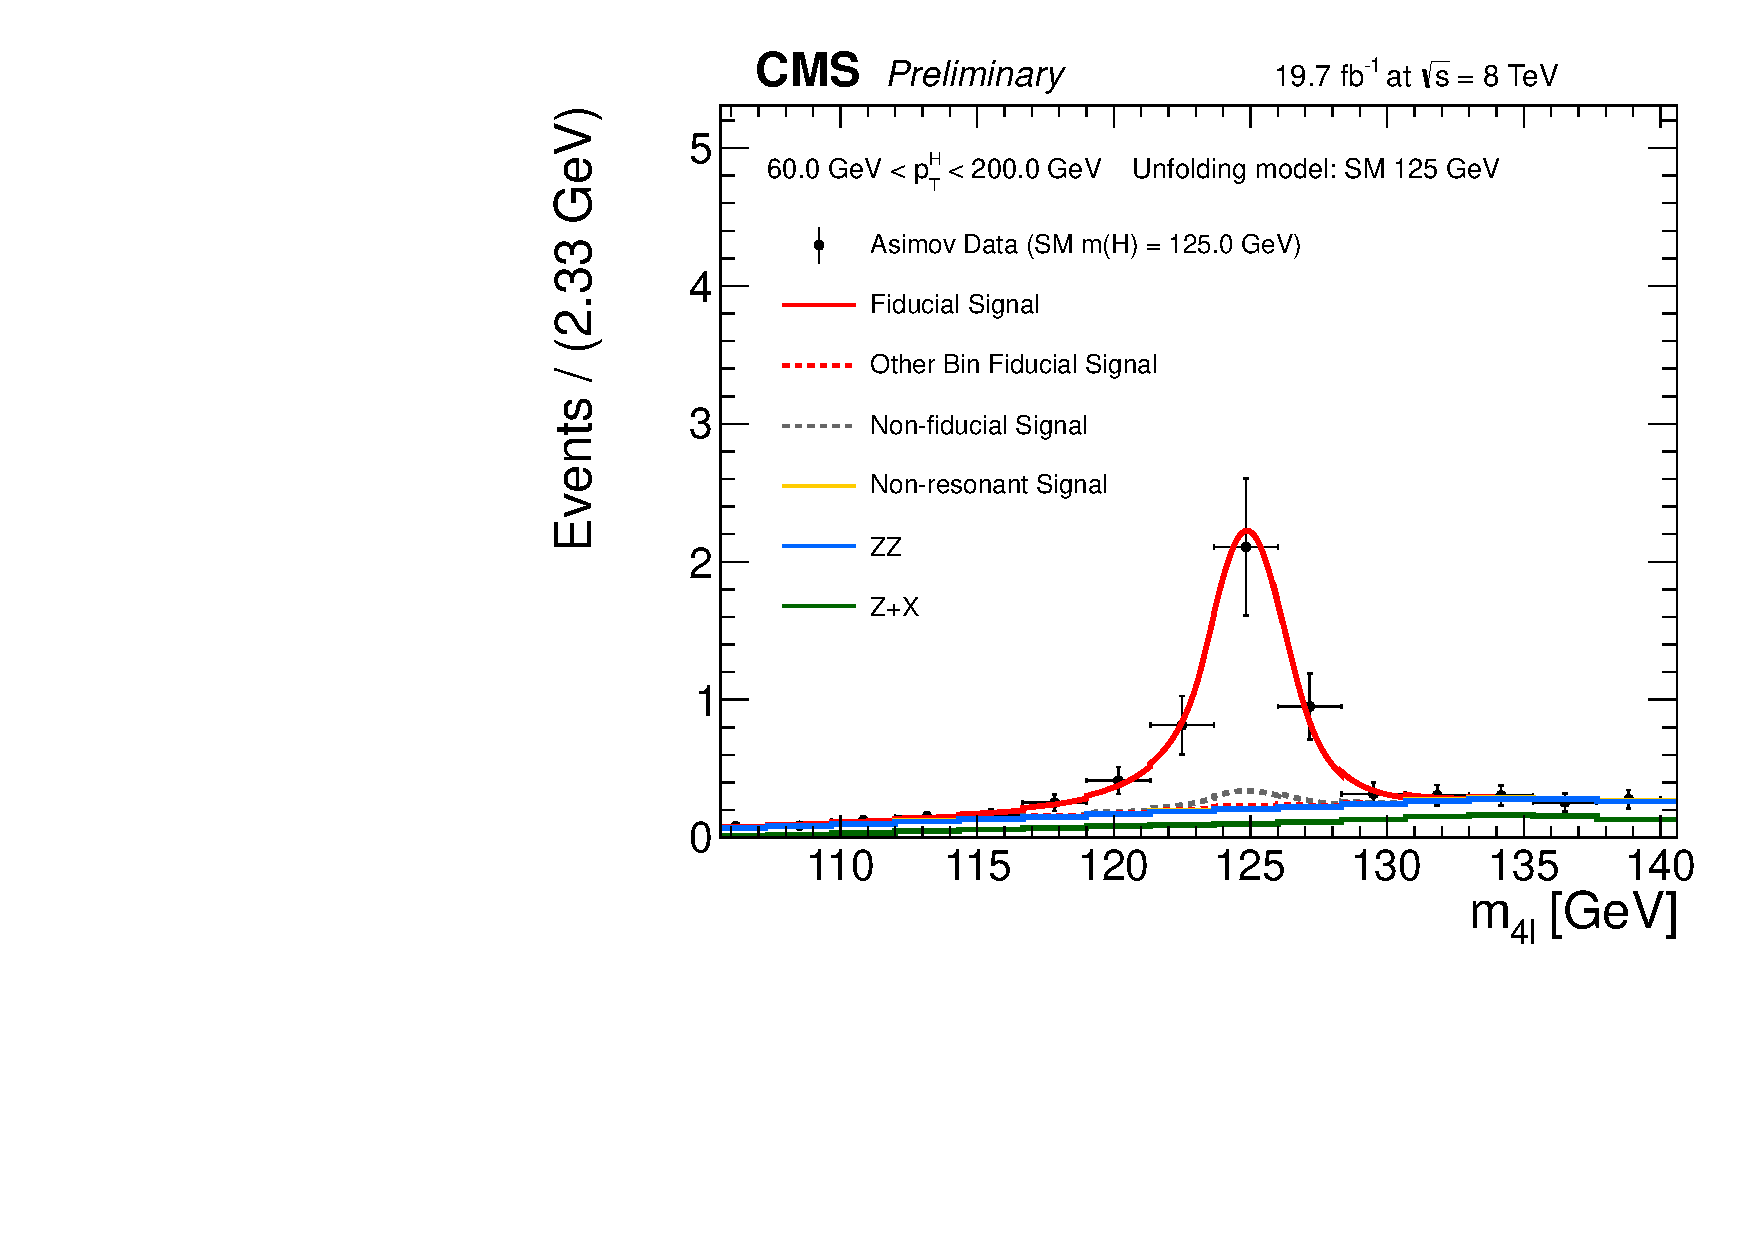
\includegraphics[width=0.40\textwidth,angle=0]{Plots/asimovdata_SM_125_v2_unfoldwith_SM_125_v3_pT4l_4l_recobin3.pdf}
       \label{fig:sigfits-asimov-SM-pT4l-4l:d}
    } \\
   \subfigure[$80.0 \GeV < \pt(\mathrm{H}) < 120.0 \GeV$]{
      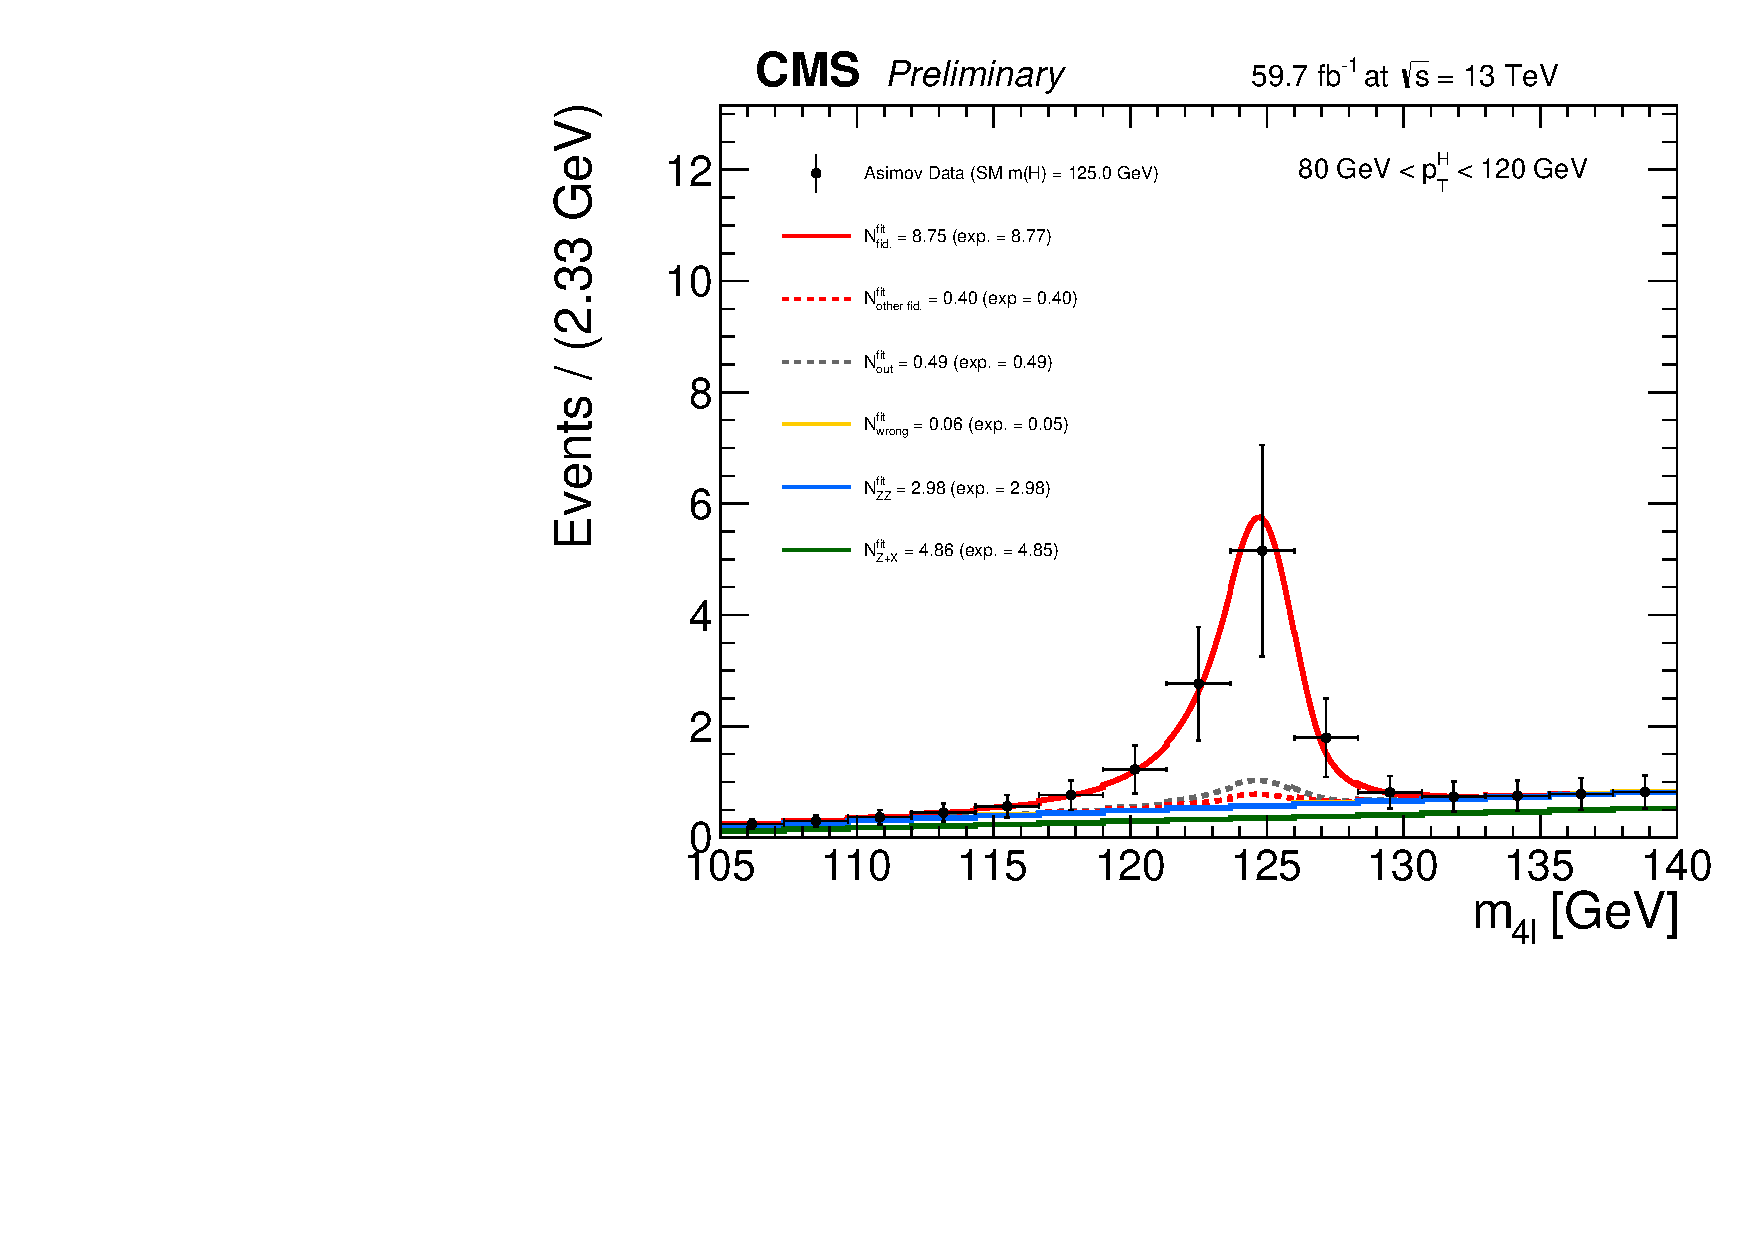
\includegraphics[width=0.40\textwidth,angle=0]{Plots/asimovdata_SM_125_v2_unfoldwith_SM_125_v3_pT4l_4l_recobin4.pdf}
       \label{fig:sigfits-asimov-SM-pT4l-4l:b}
    } 
    \subfigure[$120.0 \GeV < \pt(\mathrm{H}) < 200.0 \GeV$]{
      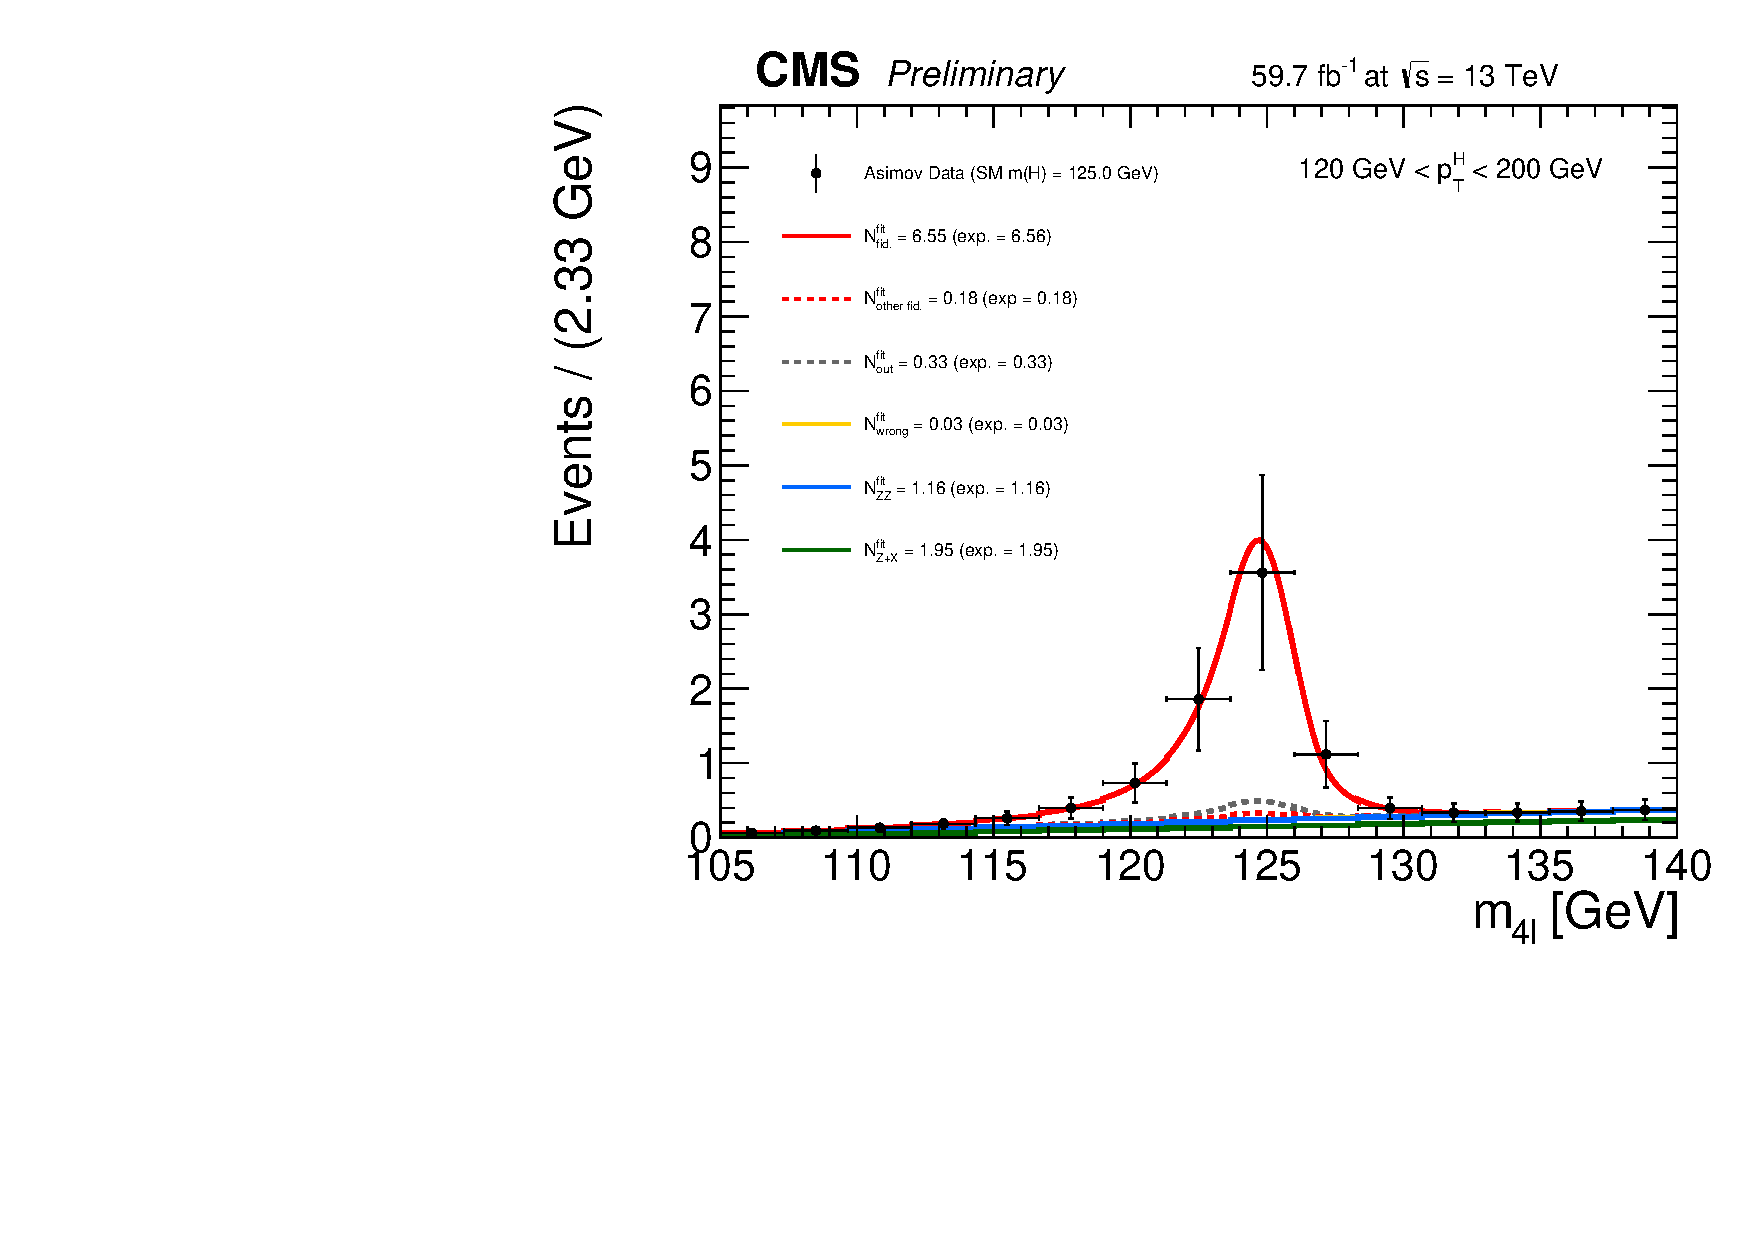
\includegraphics[width=0.40\textwidth,angle=0]{Plots/asimovdata_SM_125_v2_unfoldwith_SM_125_v3_pT4l_4l_recobin5.pdf}
       \label{fig:sigfits-asimov-SM-pT4l-4l:c}
    } \\  
    \subfigure[$200.0 \GeV < \pt(\mathrm{H}) < 13000.0 \GeV$]{
      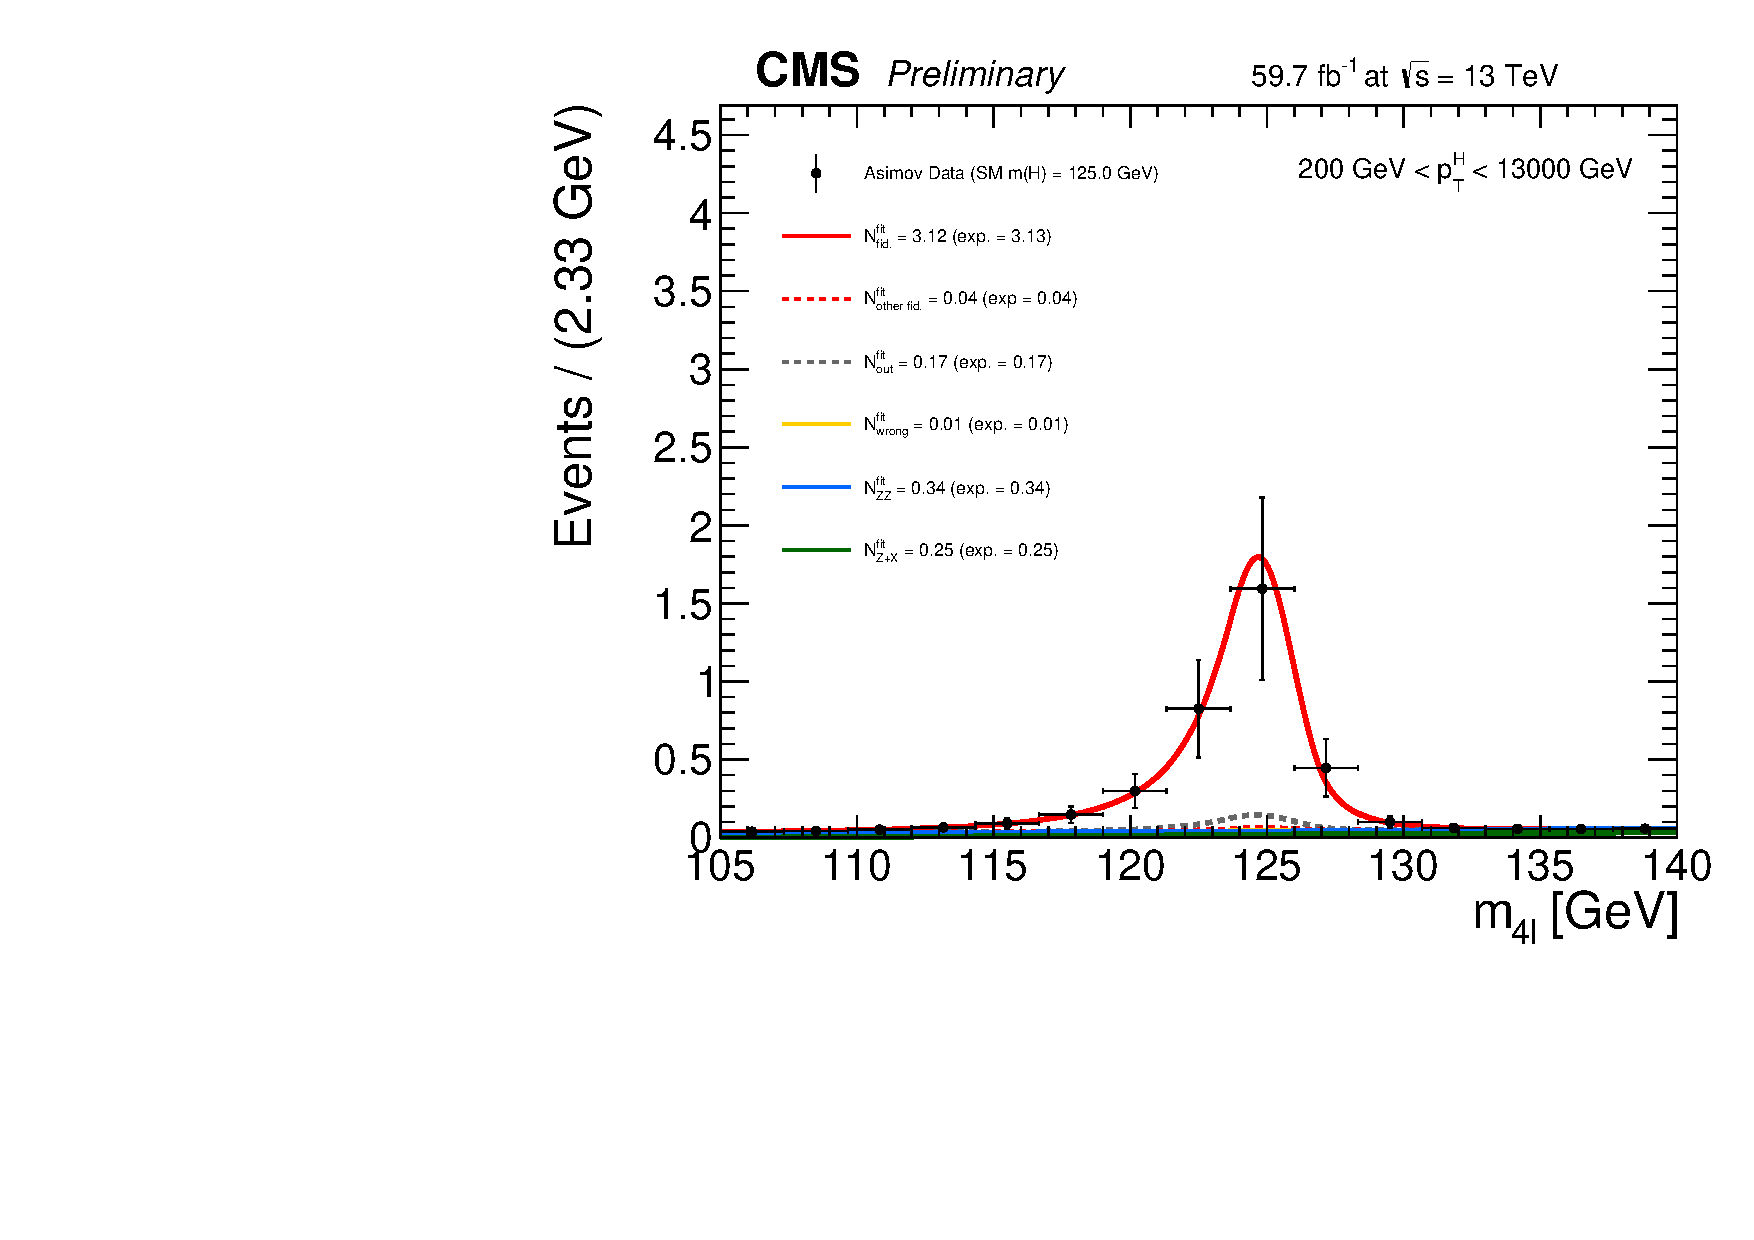
\includegraphics[width=0.40\textwidth,angle=0]{Plots/asimovdata_SM_125_v2_unfoldwith_SM_125_v3_pT4l_4l_recobin6.pdf}
       \label{fig:sigfits-asimov-SM-pT4l-4l:d}
    } \\
	  
	  \caption{Four lepton mass distributions for an Asimov dataset generated using SM cross section values and SM efficiencies where the gg$\rightarrow$H prediction
    is from {\sc powheg+JHUgen} and resulting fitted values of the signal and background pdfs in different bins of $\pt(\mathrm{H})$ (all final states combined).}
  \label{fig:sigfits-asimov-SM-pt4l-4l}
  \end{center}
\end{figure}

\clearpage
